\title{CS3210 Parallel Computing\\Assignment 2 Report\\[3ex]\textbf{Discrete Particle Simulation with MPI}}
\author{Keven Loo Yuquan \& Lee Yong Jie, Richard}
\date{}

\documentclass[12pt]{article}

% Margins
\usepackage[margin=2cm]{geometry}
% Math and symbols
\usepackage{amsmath}
\usepackage{amssymb}
% Syntax highlighting
\usepackage{minted}
% Inclusion of pictures
\usepackage{graphicx}
\graphicspath{{./reportAssets/}{./processedGpuResults/}{./processedCpuResults/}}
% Better looking underlines
\usepackage{soul}
\setuldepth{Parallel}
% Combine texttt & textbf
\usepackage{bold-extra}
% No paragraph indentations
\setlength{\parindent}{0pt}
% Merge rows of table
\usepackage{multirow}
% Fixed tables
\usepackage{tabularx}
% LaTeX is dumb at deciding where figures should go
\usepackage{float}
% Enable support for coloured text blocks
\usepackage[dvipsnames]{xcolor}
% Enable URLs
\usepackage{hyperref}
% Enable references on the TOC
\usepackage[nottoc,numbib]{tocbibind}
% Enable customized lists
\usepackage{enumitem}

% \bf formats a chunk of text to both texttt and textbf
\newcommand{\bt}[1]{\texttt{\textbf{#1}}}
% Center-aligned column
\newcolumntype{C}{>{\centering\arraybackslash}X}

\begin{document}
\maketitle
\setcounter{tocdepth}{1}
\tableofcontents

\pagebreak
\section{MPI Program Design}

The discrete particle simulation is implemented fully in MPI with the master-slave pattern. The overall architecture of the simulator is summarised in Figure \ref{fig:simulator-design} below.

\begin{figure}[H]
    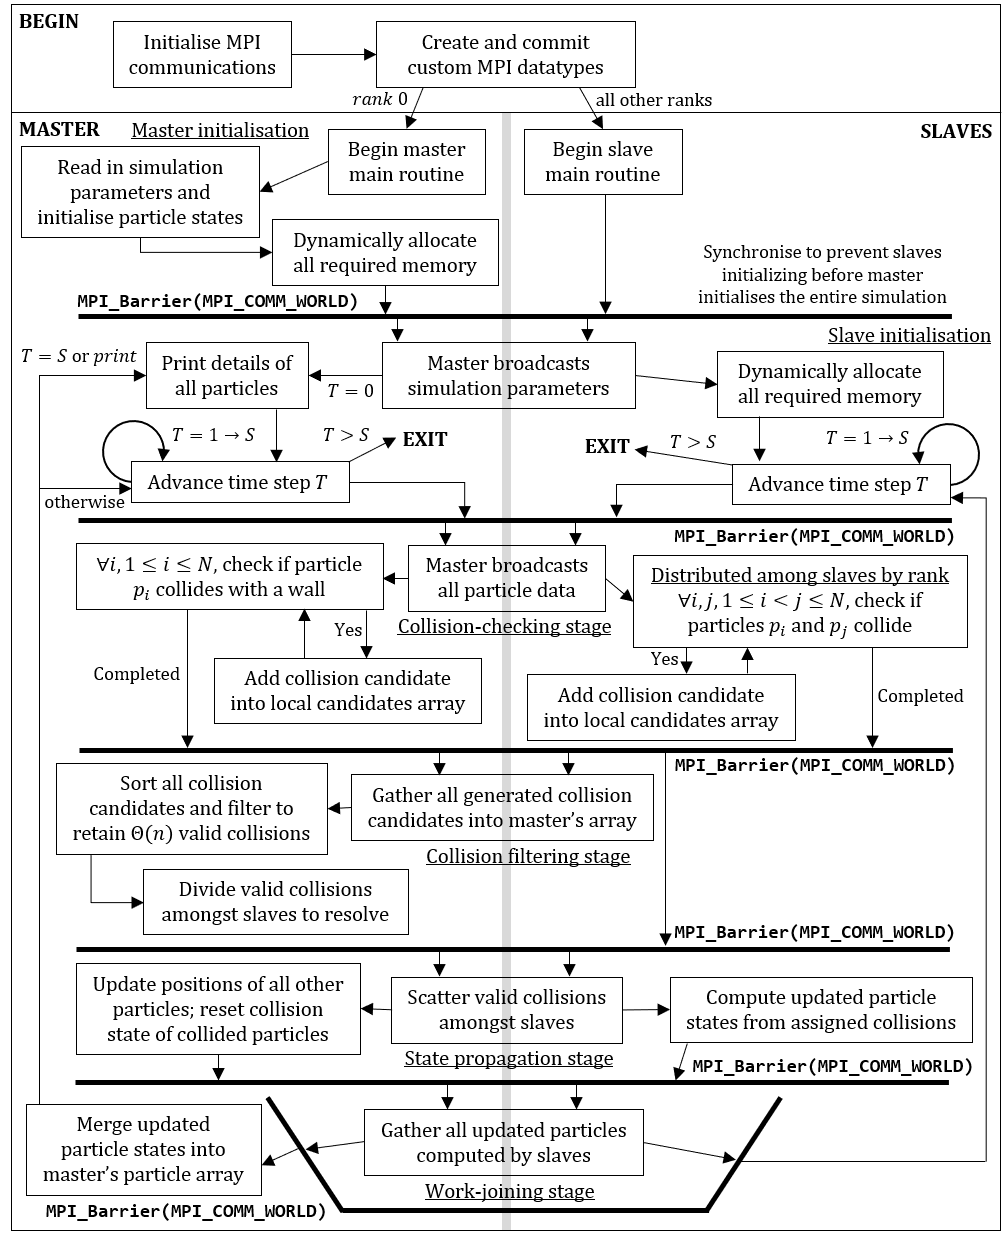
\includegraphics[width=0.94\textwidth]{chap1Flowchart-MPI}
    \centering
    \caption{Overall simulator design for MPI implementation}
    \label{fig:simulator-design}
\end{figure}

\pagebreak

\section{Implementation Assumptions and Details}

\subsection{Assumptions}

There are no changes to the assumptions made in the discrete particle simulation from the CUDA implementation. They are reproduced here for convenience.

\begin{enumerate}
	\item A particle is involved in no more than one collision per time step.
	\begin{itemize}
		\item Implications
		\begin{enumerate}
			\item If a particle collides with a wall after any collision, it is placed at the wall at the end of that time step, and will immediately collide with the wall at the beginning of the next time step
			\item If particle $P$ collides with a particle $Q$ after any collision, it will phase through the particle $Q$ for the remainder of this time step, or will ignore $Q$ the next time step if they happen to overlap
		\end{enumerate}
	\end{itemize}
	\item All collisions between particles and with the wall are elastic (kinetic energy and momentum are conserved). 
	\item It is possible to fit all $N$ particles of radius $r$ into the square of length $L$ without overlapping.
	\begin{itemize}
		\item Implication
		\begin{enumerate}
			\item The simulation exits if one of these two conditions fail: $L < 2r$ (not possible to fit a single particle) or $Nr^2 > L^2$ (not possible to pack $N$ particles in a \ul{grid arrangement} in a square with area $L^2$)
		\end{enumerate}
	\end{itemize}
	\item The set of possible collisions $C$ satisfies a \textbf{total ordering}.
	\begin{itemize}
		\item Implication
		\begin{enumerate}
			\item For each time step $T$, it is possible to sort all collision candidates by this total ordering to determine which collisions should be prioritised over others.
		\end{enumerate}
	\end{itemize}
\end{enumerate}

\pagebreak

\subsection{Implementation Details}

Changes in general implementation details from the previous report are in \textcolor{blue}{blue}.

\begin{enumerate}
	\item If the initial state of particles are not provided, particles are generated with initial random positions and velocities using a \textbf{uniform distribution}.
	\begin{enumerate}
		\item We use the pseudo-random number generator function \texttt{rand} in the C library seeded with the number 3210.
		\item Particles are placed randomly in the square without overlapping.
	\end{enumerate}
	\item Each particle keeps track of its own state: $\textrm{ID}, x, y, v_x, v_y, \textcolor{blue}{w_c, p_c}$.
	\item Our simulation has an additional parameter \texttt{SLOW\_FACTOR} in \texttt{simulator.cu} that increases the granularity of the simulation for greater accuracy. \label{slow-factor-ref}
	\begin{enumerate}
		\item Setting \texttt{SLOW\_FACTOR} to an integer $>1$ slows the initial velocities of all particles by that factor. \texttt{SLOW\_FACTOR} should be set to a power of two to avoid introducing additional floating-point errors when dividing the particles’ velocities.
		\item The number of steps of the simulation is multiplied by \texttt{SLOW\_FACTOR} to compensate, i.e. each original step now corresponds to \texttt{SLOW\_FACTOR} ``micro-steps".
	\end{enumerate}
	\item Collisions are of two types: particle-wall collisions or particle-particle collisions. We describe a particle-wall collision as ($P$, \textcolor{blue}{\texttt{WALL}}) and a particle-particle collision as ($P$, $Q$). \textcolor{blue}{\texttt{WALL} is defined with \texttt{\#define WALL -1}.}
	\begin{enumerate}
		\item As particle-particle collisions are symmetric (i.e. $P$ collides with $Q$ $\iff$ $Q$ collides with $P$), we generate these collisions such that $P$ is the particle with lower integer ID to avoid duplicates.
	\end{enumerate}
	\item When sorting collision candidates with the C library function \texttt{qsort}, we enforce this total ordering in the function \texttt{cmpCollision}. For two collision candidates  $C_1$ and $C_2$,
	\begin{itemize}
		\item[$\blacksquare$] $C_1 < C_2$ if $C_1$ occurs before $C_2$ (priority by time)
		\item[$\blacksquare$] If $C_1$ and $C_2$ occur at the same time
		\begin{itemize}
			\item[$\square$] $C_1 < C_2$ if ID of $P$ in $C_1$ $<$ ID of $P$ in $C_2$ (priority by ID)
			\item[$\square$] If $C_1$ and $C_2$ both involve the same particle $P$
				\begin{itemize}
					\item[$\blacksquare$] $C_1 < C_2$ if $C_1$ is a wall collision (priority by type)
					\item[$\blacksquare$] If $C_1$ and $C_2$ are both particle-particle collisions
						\begin{itemize}
							\item[$\square$] $C_1 < C_2$ if ID of $Q$ in $C_1$ $<$ ID of $Q$ in $C_2$ (priority by ID)
						\end{itemize}
				\end{itemize}
		\end{itemize}
	\end{itemize}
	\item For each particle in each time step, we check once if the particle collides with any of the four walls.
	    \begin{enumerate}
	        \item A particle is treated to have collided with a wall if it would come within a distance of $\epsilon = $ \texttt{1E-8} to the wall within that time step.
	    \end{enumerate}
	\item All possible particle-particle collision pairs are checked for each time step. The total number of collision checks performed is thus
	\begin{align*}
	N_{potential\ collisions} 	&= N_{wall-particle} + N_{particle-particle} \\
						&= N + \frac{N(N-1)}{2} \\
						&= \Theta (N^2)
	\end{align*}
	\item Particle-wall collisions are checked by solving the trajectory equation of a particle and the position equations of the wall. The equations of the walls are $x = 0, x = L, y = 0, y = L$.
	\item \label{trajectory-calc} Particle-particle collisions are checked by solving trajectory equations of two particles during the given time step.\\
	
	Consider two particles $P$, $Q$ during a given time step $0 \leq \Delta t \leq 1$. From Pythagoras’ theorem, the distance between them is
	$$d = \sqrt{\left( \left( x_Q + v_{xQ} \Delta t \right) - \left( x_p + v_{xP} \Delta t \right) \right)^2 +
		\left( \left( y_Q + v_{yQ} \Delta t \right) - \left( y_p + v_{yP} \Delta t \right) \right)^2}$$
	or re-written in terms of deltas (differences in state)
	$$d = \sqrt{\left( \Delta x + \Delta v_x \Delta t \right)^2 +
		\left( \Delta y + \Delta v_y \Delta t \right)^2}$$
    \\
	The particles intersect when $d = 2r$, i.e. the particles touch at their circumference, hence by expanding and collecting terms we get the quadratic equation of form $A (\Delta t)^2 + B \Delta t + C = 0$,
	\begin{align*}
		\Delta x^2 + 2 \Delta x \Delta v_x \Delta t + \Delta v_x^2 (\Delta t)^2 + \Delta y^2 + 2 \Delta y \Delta v_y \Delta t + \Delta v_y^2 (\Delta t)^2 = (2r)^2 \\
		\implies (\Delta v_x^2 + \Delta v_y^2) (\Delta t)^2 + (2 \Delta x \Delta v_x + 2 \Delta y \Delta v_y) \Delta t + (\Delta x^2 + \Delta y^2 - 4r^2) = 0
	\end{align*}
	
	We observe that $A = (\Delta v_x^2 + \Delta v_y^2) > 0$ and thus the curve $y = d(\Delta t)$ is concave up. The discriminant for this quadratic equation, $B^2 - 4AC$, is
	$$\textrm{discriminant} = (2 \Delta x \Delta v_x + 2 \Delta y \Delta v_y)^2 - 4(\Delta v_x^2 + \Delta v_y^2)(\Delta x^2 + \Delta y^2 - 4r^2)$$
	
	If this discriminant is $\geq 0$, then the particles collide for some value of $\Delta t$, and we solve for this $\Delta t$. There are two possible roots,
	$$\Delta t = \frac{-B \pm \sqrt{\textrm{discriminant}}}{2A}$$
	
	Since the quadratic curve is concave up, we only compute and examine the first root (when the particles are approaching each other). This is
	$$\Delta t = \frac{-B - \sqrt{\textrm{discriminant}}}{2A}$$
	
	If $0 \leq \Delta t \leq 1$, then particles $P$, $Q$ collide during this time step.
	
	Note that, it is possible for $\Delta t < 0$ - this corresponds to cases where particles are overlapping from a previous step. We do not consider these as collisions in the current step and let these two particles phase through each other.
	\item To ensure the collision candidates array \textcolor{blue}{in the master process} can accommodate $\Theta(N^2)$ potential collisions (in the limit of large $N$ when particle-particle collisions dominate), we dynamically allocate an array with sufficient space to store $N^2 / 2$ \texttt{collision\_t} structs.
	\item \textcolor{blue}{To allow our \texttt{particle\_t} and \texttt{collision\_t} structs to be transmitted by MPI, we created the matching MPI datatypes \texttt{MP\_PARTICLE} and \texttt{MP\_COLLISION}.}
	\begin{itemize}
	    \item \textcolor{blue}{Note that the \texttt{MPI\_} prefix is reserved for the OpenMPI library, hence the use of the \texttt{MP\_} prefix instead.}
	\end{itemize}
	\item \textcolor{blue}{The structs themselves have also been modified for the MPI implementation.}
	\begin{itemize}
	    \item \textcolor{blue}{Due to the distributed-memory nature of MPI, the \texttt{particle\_t} pointers in \texttt{collision\_t} are no longer useful - they have been replaced with two \texttt{int}s, specifying the particle(s) involved in the collision by their ID}
	    \item \textcolor{blue}{The original \texttt{particle\_t} struct resulted in alignment issues during transmission with MPI, due to \textbf{structure padding} in C. To mitigate this, a dummy \texttt{int} member \texttt{dummy} was added after the \texttt{id} member to align the \texttt{double} members along 4-byte word boundaries.}
	\end{itemize}
\end{enumerate} 

\pagebreak

\section{Parallelisation Strategy}

\subsection{OpenMP and CUDA Implementation}
There are no changes to the parallelisation strategy of our OpenMP and CUDA implementations from Assignment 1. Please refer to the reports for Parts 1 and 2 of Assignment 1 for details.

\subsection{Task Decomposition}
\label{subsection:task-decomposition}
Similar to the CUDA implementation, the computation of each step comprises three distinct stages, two of which contain multiple tasks:
\begin{itemize}
    \item Collision-checking: (1) particle-wall and (2) particle-particle
    \item Filtering: prioritising valid collisions
    \item State propagation: (1) resolving collisions and (2) updating positions
\end{itemize}

These three stages must be completed serially for each step, which requires inter-stage synchronisation points. However, within each stage, it is possible to compute the tasks in parallel, by dividing the work amongst MPI processes.

\subsection{Programming Pattern}
Since the tasks in the simulation have significant dependencies and thus require heavy coordination, we decided to implement our MPI program with the \textbf{master-slave} pattern for $P$ processes.\\

The process with rank $0$ is designated the \textbf{master process} and will be responsible for:
\begin{itemize}
    \item Reading in the simulation parameters and initial particle states, initialising particles with random positions and velocities using a \textbf{uniform random distribution} if not provided
    \item Performing all printing operations of the simulation state to \texttt{stdout}
    \item Maintaining the updated simulation state at each time step $S$
    \item Assigning work to slave processes, and retrieving all work after computation has completed
\end{itemize}

All other processes with ranks $1, 2, ..., P - 1$ are designated \textbf{slave processes}, and will only perform computation.

\subsection{Master-Slave Work Division}
Since the master process is heavily involved in coordination, we assign it small tasks. This allows the master to perform some work whilst the slaves complete the bulk of the computation. The computation routines for the master are: 
\begin{enumerate}
    \item \texttt{MASTER\_checkWallCollisions} - checks all $N$ particle-wall collisions
    \item \texttt{MASTER\_updateParticles} - updates state of uncollided particles; resets collision status of collided particles
\end{enumerate}

In contrast, we assign large tasks to the slave processes, who will divide up the computation amongst themselves (the data distribution is detailed in section \ref{subsection:data-distribution}). The computation routines for the slaves are:
\begin{enumerate}
    \item \texttt{SLAVE\_checkCollisions} - checks all $\Theta(N^2)$ particle-particle collision pairs
    \begin{itemize}
        \item \textbf{Implicit assignment} of particle-particle collision pairs to each slave - each slave determines the computations it performs based on its rank 
    \end{itemize}
    \item \texttt{SLAVE\_resolveCollisions} - resolves assigned valid collisions by computing the updated state of the involved particles
    \begin{itemize}
        \item \textbf{Explicit assignment} of valid collisions to each slave - master assigns each slave a unique set of collisions to resolve using \texttt{MPI\_Scatterv}
    \end{itemize}
\end{enumerate}

For the explicit assignment of valid collisions to resolve, the master first performs an \texttt{MPI\_Scatter} to inform each slave of the number of collisions it will be assigned. The master then scatters a varying number of valid collisions to each of the slaves with the variable-message-size variant of \texttt{MPI\_Scatter}, \texttt{MPI\_Scatterv}.\\

Each of the slaves will also generate a varying number of elements (collision candidates or updated particles) from its tasks. For the master to collect all these elements, it first performs an \texttt{MPI\_Gather} to retrieve the number of items each slave will send. The master then gathers a varying number of elements from each of the slaves with the variable-message-size variant of \texttt{MPI\_Gather}, \texttt{MPI\_Gatherv}.\\

These variable-message-size variants of the collective communication operations provide more flexibility but require two additional arrays:
\begin{enumerate}
    \item \texttt{counts} - integer array with the $i$th element specifying the number of elements to send to the process with rank $i$
    \item \texttt{displs} - integer array with the $i$th element specifying the displacement
    \begin{itemize}
        \item (For \texttt{MPI\_Scatterv}) relative to the start of the send buffer of the root, at which to take the outgoing data for the process with rank $i$
        \item (For \texttt{MPI\_Gatherv}) relative to the start of the receive buffer of the root, at which to place the incoming data from the process with rank $i$
    \end{itemize}
\end{enumerate}

For \texttt{MPI\_Gatherv}, the first array \texttt{count} is constructed from the initial collective communication operation, whereas it is built by the master for \texttt{MPI\_Scatterv}. The following are the helper routines executed by the master for these:
\begin{enumerate}
    \item \texttt{MASTER\_buildDisplacement} - builds the displacement array \texttt{displs} from the counts array \texttt{counts} obtained from an earlier call to \texttt{MPI\_Gather}
    \item \texttt{MASTER\_divideCollisions} - divides the number of valid collisions amongst all the slaves, building both \texttt{counts} and \texttt{displs} in the process
\end{enumerate}

As part of the coordination role performed by the master, it also executes the following additional routines:
\begin{enumerate}
    \item \texttt{MASTER\_filterCollisions} - after collecting all collision candidates into the master's array, sorts and filters to retain the valid collisions
    \begin{itemize}
        \item \texttt{MASTER\_buildDisplacement} returns the total number of elements sent by all processes in \texttt{MPI\_Gatherv}, which is used to update the master's \texttt{numCollisions}
        \item Filtering is only performed by the master due to its inherently serial nature (since selecting an earlier collision may invalidate later collisions, as a particle can only collide once in a given time step)
    \end{itemize}
    \item \texttt{MASTER\_mergeResolvedParticles} - after collecting all particles updated from resolving collisions, copies the updates into the master's particle array
    \item \texttt{MASTER\_printAll} - prints the simulation state to \texttt{stdout}
\end{enumerate}

\subsection{Task and Data Distribution}
\label{subsection:data-distribution}
Since the slaves will only check particle-particle collision pairs for $p_i$ and $p_j$ where $0 \leq i < j < n$ (where $i, j$ are the indices of the particles in the array \texttt{ps}), we can visualise all the computations to be performed for each time step as the section above the upper diagonal of a $N \times N$ matrix, as shown in Figure \ref{fig:collisionMatrix}. This is similar to the CUDA implementation.

\begin{figure}[H]
    \centering
    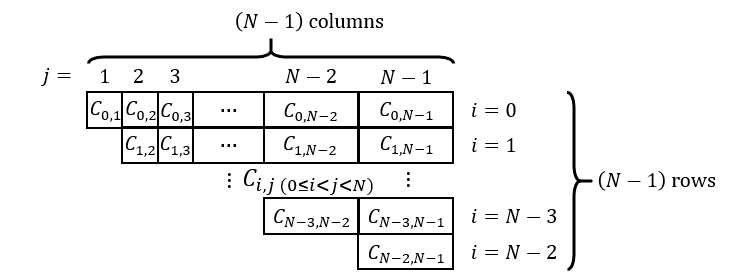
\includegraphics[width=1.0\textwidth]{reportAssets/chap3ppCollisionMatrix.png}
    \caption{Matrix of particle-particle computations}
    \label{fig:collisionMatrix}
\end{figure}

We considered assigning evenly-sized blocks of rows of computation to each of the slaves. However, this leads to an uneven distribution of work, since the number of potential collisions to check in the $i$th row is $(N - 1 - i)$. Since the master cannot proceed to filter collisions until all slaves have completed, our MPI program will be severely bottlenecked by the (slowest) slave assigned the block with the longest set of rows.\\

We then considered letting the master dynamically assign one row of computation to each slave, collecting the result when the row is complete, before assigning another, until all rows are fully computed.\\

However, this will increase the granularity of the tasks and the amount of communications required, increasing the overhead substantially. Furthermore, it prevents the master from performing any useful work alongside the slaves, which necessitates distributing the particle-wall collision checks amongst the slaves as well.\\

Therefore, similar to our CUDA implementation, since the upper half of the matrix resembles a triangle, we decided to "fold" the lower half of the matrix onto the upper half, by reflecting it in both axes and stitching it together to form a rectangle, as shown in Figure \ref{fig:collisionMatrixFolded}.

\begin{figure}[H]
    \centering
    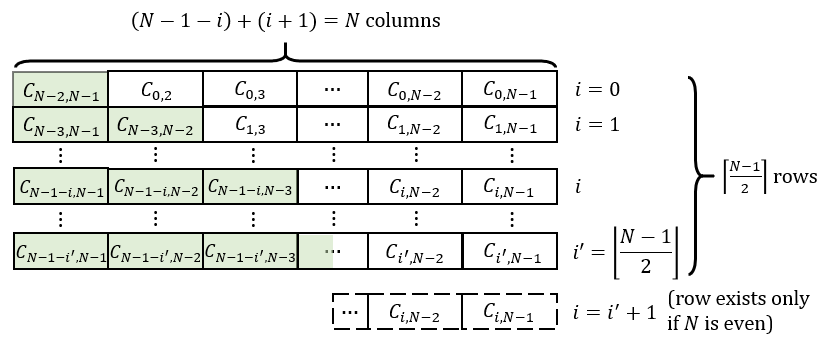
\includegraphics[width=1.0\textwidth]{reportAssets/chap3ppCollisionMatrixFolded.png}
    \caption{Folded matrix of particle-particle computations}
    \label{fig:collisionMatrixFolded}
\end{figure}

This produces a rectangular matrix with $ceil((N - 1) / 2)$ rows and exactly $N$ columns, with the shaded green cells denoting the reflected portion. Note that if $(N - 1)$ is odd, i.e. $N$ is even, that the matrix will not fold perfectly and there will be a leftover (last) row with only $N / 2$ computations.\\

Then, we performed \textbf{blockwise assignment} of the rows of computation to each of the slave processes by their rank, as shown in Figure \ref{fig:collisionMatrixFoldedAssignment}.

\begin{figure}[H]
    \centering
    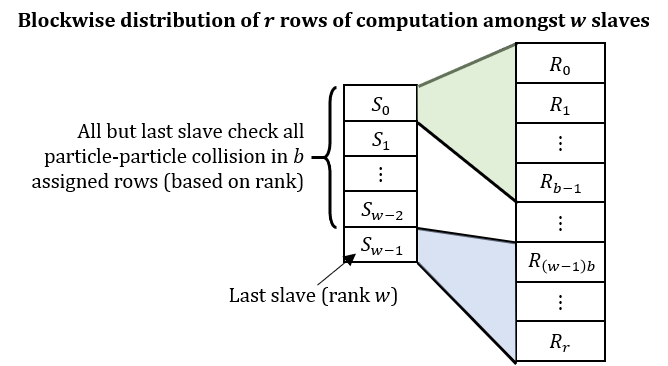
\includegraphics[width=0.95\textwidth]{reportAssets/chap3collisionMatrixDecomposition.png}
    \caption{Blockwise assignment of rows of computation to slaves}
    \label{fig:collisionMatrixFoldedAssignment}
\end{figure}

During the state propagation stage, the master assigns valid collisions to slaves with a \textbf{blockwise assignment}, as shown in Figure \ref{fig:collisionArrayAssignment}.

\begin{figure}[H]
    \centering
    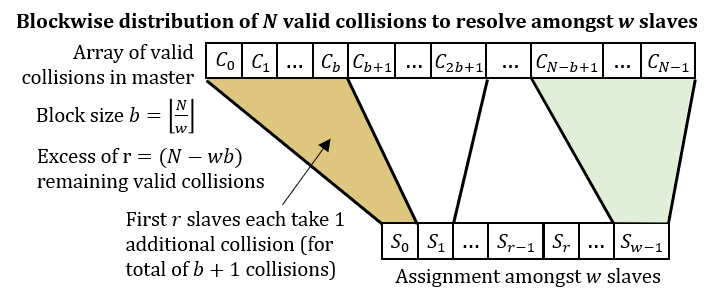
\includegraphics[width=0.95\textwidth]{reportAssets/chap3collisionArrayDecomposition.png}
    \caption{Blockwise assignment of rows of computation to slaves}
    \label{fig:collisionArrayAssignment}
\end{figure}

\pagebreak

\subsection{Memory Considerations}
Since each MPI process has an independent memory space, certain information about the simulation parameters must be replicated across all processes before beginning any computation. These include:
\begin{itemize}
    \item Simulation parameters \texttt{n}, \texttt{l}, \texttt{r}, \texttt{s}
    \item Derived simulation parameters \texttt{minMargin}, \texttt{maxMargin}, \texttt{max} for the boundaries of the square.
\end{itemize}

These are broadcast by the master process after initialisating the simulation.\\

All processes also store the following information required for computation.
\begin{itemize}
    \item Integer counter for the number of collisions \texttt{numCollisions}
    \begin{itemize}
        \item This is reset to 0 at the beginning of each time step, then incremented locally for each process as it generates collision candidates
        \item The master's variable will then be updated with the total count across all processes, and then the total number of valid collisions after filtering
        \item As the master assigns valid collisions, \texttt{numCollisions} in the slaves are updated to reflect the number of valid collisions assigned to each slave
    \end{itemize}
    \item Array of $N$ particles \texttt{ps}
    \begin{itemize}
        \item The master's particle array is treated as the \textbf{source of truth}, and is broadcast to all processes at the beginning of a time step
        \item This was done to avoid complicating the master routine having to send differing data to each slave for each task, since
        \begin{enumerate}[label=(\arabic*)]
            \item the particles required during collision-checking varies non-trivially on the rank of each slave (as the computation matrix is folded), and
            \item the particles updated by each slave during collision resolution varies in a non-deterministic manner with each time step
        \end{enumerate}
        \item Whilst this incurs greater communication overhead, it ensures that all slaves see the same the same simulation state; furthermore, \texttt{MPI\_Bcast} uses an efficient tree broadcast algorithm for good network utilisation
        \item It also avoids the need for the slaves to merge in the set of received particles into their particle array, since the \texttt{collision\_t} struct now references particles by their ID (index in the array)
    \end{itemize}
    \item Buffer array of $N$ particles \texttt{pBuffer}
    \begin{itemize}
        \item This buffer is used by slaves to store the updated particles computed from resolving collisions
        \item This buffer is only used by the master to store all the updated particles gathered from the slaves with \texttt{MPI\_Gatherv}, to update the master's copy of the particle array with \texttt{MASTER\_mergeUpdatedParticles}
    \end{itemize}
    \item Array of collision candidates \texttt{cs}
    \begin{itemize}
        \item This array is used by all processes to store the collision candidates each process generates
        \item This array is then used by the master to store all the collision candidates gathered from itself and the slaves with \texttt{MPI\_Gatherv}, for filtering
        \item The array is then re-used by the slaves to store the valid collisions assigned by the master to resolve
        \item Its size is $N^2 / 2$ in the master and $N^2 / (2 \times W)$ in each of the $W = P - 1$ slaves
    \end{itemize}
\end{itemize}

The master process stores the following additional information, as part of its role involves coordinating the entire simulation:
\begin{itemize}
    \item Array of $P$ integers \texttt{numItems}
    \item Array of $P$ integers \texttt{displc}
    \item Array of $N$ integers describing collision states of all particles, \texttt{states}
    \begin{itemize}
        \item The $i$th integer describes the collision state of the $i$th particle
        \item \texttt{NOT\_COLLIDED = 0; COLLIDED = 1}
        \item This array is only required by the master for filtering valid collisions and is never transmitted
        \item The collision states of all particles are reset back to \texttt{NOT\_COLLIDED} at the end of a time step in \texttt{MASTER\_updateParticles}
    \end{itemize}
\end{itemize}

\subsection{Synchronisation Requirements}
Both the OpenMP and CUDA programming models rely heavily upon shared memory. More specifically,
\begin{itemize}
    \item In OpenMP, most variables are visible to all threads by default, unless explicitly specified otherwise by the programmer
    \item In CUDA, all threads have access to the same global and constant memory; additionally, all threads in the same block have access to a common shared memory
\end{itemize}

In our OpenMP and CUDA implementations, we actively made use of shared memory constructs and thus this necessitates certain synchronisation mechanisms to avoid race conditions. Specifically,
\begin{itemize}
    \item In OpenMP, all threads added new collision candidates to a common array then incremented a shared counter
    \begin{itemize}
        \item This was marked a critical section with \texttt{\#pragma omp critical}
    \end{itemize}
    \item In CUDA, threads of the \texttt{checkWallCollision} and \texttt{checkCollision} kernels may be required to add a new collision to an array in global memory and update the \texttt{numCollisions} counter (also in global memory)
    \begin{itemize}
        \item To prevent race conditions, we used the atomic function \texttt{atomicAdd} from the CUDA library to increment \texttt{numCollisions}
        \item Since \texttt{atomicAdd} returns the previous value of the counter, this gives each thread a unique index in the array to add its collision candidate to
    \end{itemize}
\end{itemize}

\pagebreak

In contrast, the master and slave processes in our MPI implementation all possess independent memory spaces. Since each process works with its own copy of its variables and data, race conditions are not possible and therefore synchronisation mechanisms to prevent concurrent access are not required.\\

However, it is essential that all processes are executing in lockstep in the correct stage, as outlined in section \ref{subsection:task-decomposition}, since dependencies exist between tasks in different stages. Otherwise, the following errors could occur:
\begin{itemize}
    \item Slaves beginning initialisation before the master broadcasts the simulation parameters, leading to segmentation faults
    \item Slaves proceeding to the next stage of computation with stale data before the master completes some computation
\end{itemize}

To achieve this, we explicitly made use of \texttt{MPI\_Barrier} to synchronise the master and all slaves prior to the beginning of every stage and collective communication operation. Note that this was only possible due to the use of blocking communication operations.

\subsection{Network Considerations}
For a distributed-memory programming model such as MPI, being sensitive to the network layout of the processing elements is also critical, since message-passing occurs on the network.\\

We hypothesise that the network layout of the computing nodes in the Parallel-Distributed Computing Lab (COM1-B102) follows closely from their physical arrangement, as shown on the next page in Figure \ref{fig:networkLayout}.

\begin{figure}[H]
    \centering
    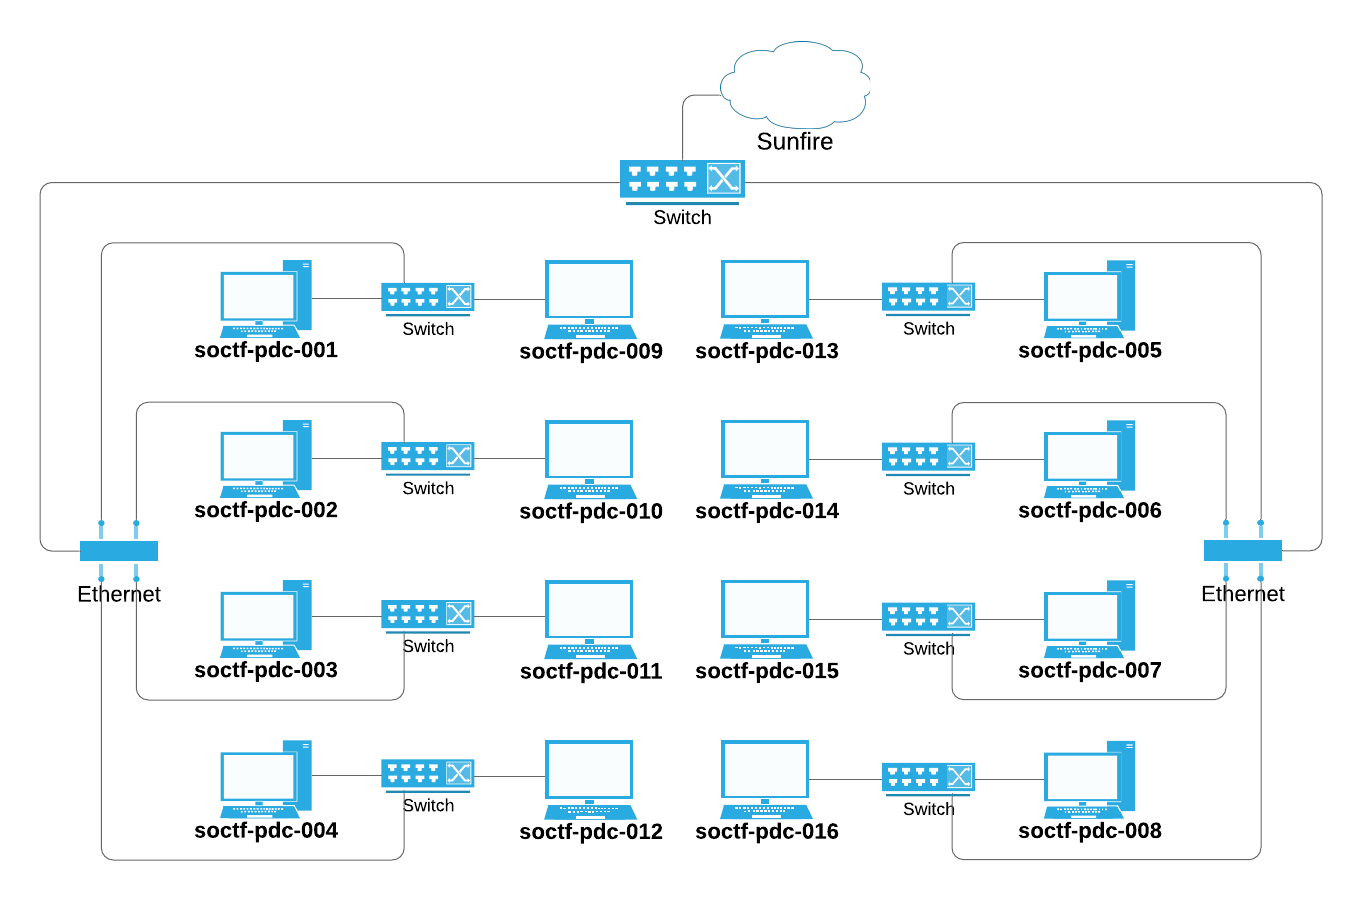
\includegraphics[width=1.0\textwidth]{reportAssets/chap3nodeNetworkLayout.png}
    \caption{Assumed network layout of computing nodes in COM1-B102}
    \label{fig:networkLayout}
\end{figure}

To minimise the effect of network latency on communication operations between MPI processes, we selected nodes in close proximity for each of our testcases.

\pagebreak

\section{Test Conditions and Testcases}

\subsection{Test Setup}

For ease of deployment, we wrote a Bash script to automate the compilation, testcase generation, profiling and transfer of results back to Sunfire with different sets of source code. The scripts can be found in the folder \texttt{/testDispatcher}.\\

Our previous sequential and parallel OpenMP implementations were benchmarked on both an Intel Xeon Silver 4114 node and an Intel i7-7700K node, specifically \ul{soctf-pdc-001} and \ul{soctf-pdc-009}. We ran the OpenMP program on 20 threads for the Xeon and 8 threads on the 7700K, which we found to produce the highest speedup with respect to our sequential implementation. \cite{assign1aref}\\

Benchmarking of our MPI implementation was done in two configurations - with the Intel Xeon Silver 4114 node, specifically \ul{soctf-pdc-001}, as the host (master) machine and with the Intel i7-7700K node, specifically \ul{soctf-pdc-009} as the host (master) machine.\\

A Python script was used to generate the input files for each of the implementations. Each testcase was run five times and the fastest execution time was retained as the datapoint for that testcase.\\

To replicate our results for a given implementation, run \bt{./run.sh} in the particular implementation's folder. It is recommended to change the target folder for the \bt{scp} command as it will automatically transfer all the results out when it is complete.

\subsection{Random Testcases}
For benchmarking, testcases ran in \textit{perf} mode and the initial states of particles were not provided. Variables of the simulation were adjusted for each testcase.\\

For each node utilised in a testcase, all logical cores of that node will be utilised to run the program, with a one-to-one mapping of each MPI process to a logical core.
\begin{itemize}
    \item This is 8 MPI processes for each Intel i7-7700K node, and 20 MPI processes for each Intel Xeon Silver 4114 node
\end{itemize}

\pagebreak

The simulation parameters of the default testcase are
\begin{itemize}
	\item $N = 1000, L=20000, r=1, S=1000$
\end{itemize}

The testcases that were executed for each implementation are as follows.
\begin{enumerate}
    \item Sequential implementation (Xeon 4114 \& i7-7700K)
	\begin{itemize}
		\item Varying $N$ only: $N = 250, 375, 500, 750, 1000, 1500, 2000$
	\end{itemize}
	
	\item Parallel OpenMP implementation - (Xeon 4114 \& i7-7700K)
	\begin{itemize}
	    \item $P = 8$ (for i7-7700K) or $P = 20$ (for Xeon 4114)
		\item Varying $N$ only: $N = 250, 375, 500, 750, 1000, 1500, 2000, 3000, 4000, 6000$
	\end{itemize}
	
	\item MPI implementation (\textbf{only Xeon 4114 nodes})
	\begin{itemize}
		\item $M$ = Xeon 4114 nodes utilised
		\item $P$ = Total number of MPI processes
		\item Varying both $N$ and $M$ together
		\begin{itemize}
			\item $N = 1k, 2k, 3k, 4k, 6k, 8k, 12k, 16k, 24k$
			\item $M = 1, 2, 4, 8 \implies P = 20, 40, 80, 160$
		\end{itemize}
	\end{itemize}
	
	\item MPI implementation (\textbf{only i7-7700K nodes})
	\begin{itemize}
		\item $M$ = i7-7700K nodes utilised
		\item $P$ = Total number of MPI processes
		\item Varying both $N$ and $M$ together
		\begin{itemize}
			\item $N = 1k, 2k, 3k, 4k, 6k, 8k, 12k, 16k, 24k$
			\item $M = 1, 2, 4, 8 \implies P = 8, 16, 32, 64$
		\end{itemize}
	\end{itemize}
\end{enumerate}

\pagebreak

\section{Execution Results}

All plots were generated with the help of R. Some of the plots are not reproduced here for brevity.\\

The processed data is available in the submission as \texttt{.csv} files in \texttt{/data/cpu}. Raw data files from the \bt{perf stat} command are available in \texttt{/data/cpu/<configType>} as text files with no extension.\\

\textbf{Due to the incredibly slow speed of the sequential implementation, data points for $N > 2k$ were extrapolated from existing data. This was also done for the large data points for the OpenMP implementation, which became difficult to benchmark above $N > 6k$.}\\

To be precise, since we have observed that the algorithm's execution time is directly proportional to $N^2$, a quadratic regression (polynomial of degree 2) was fitted onto existing data points for both the sequential and OpenMP implementations. The extrapolated data points at $N = 3k, 4k, 6k, 8k, 12k, 16k, 24k$ was obtained as a rough estimate for computation of \textit{speedup}. The $R^2$ obtained from the quadratic fits are at least $0.99991$, which is sufficiently close to $1$ and indicates that the predicted behaviour will likely resemble the actual execution time if the testcases were run.\\

Hence, all mentions of \textit{speedup} that follow (regardless of OpenMP or MPI implementation) are made with reference to the \textbf{extrapolated execution time} of the sequential algorithm.

\subsection{Extrapolated Sequential and OpenMP Results}

\begin{figure}[H]
    \centering
    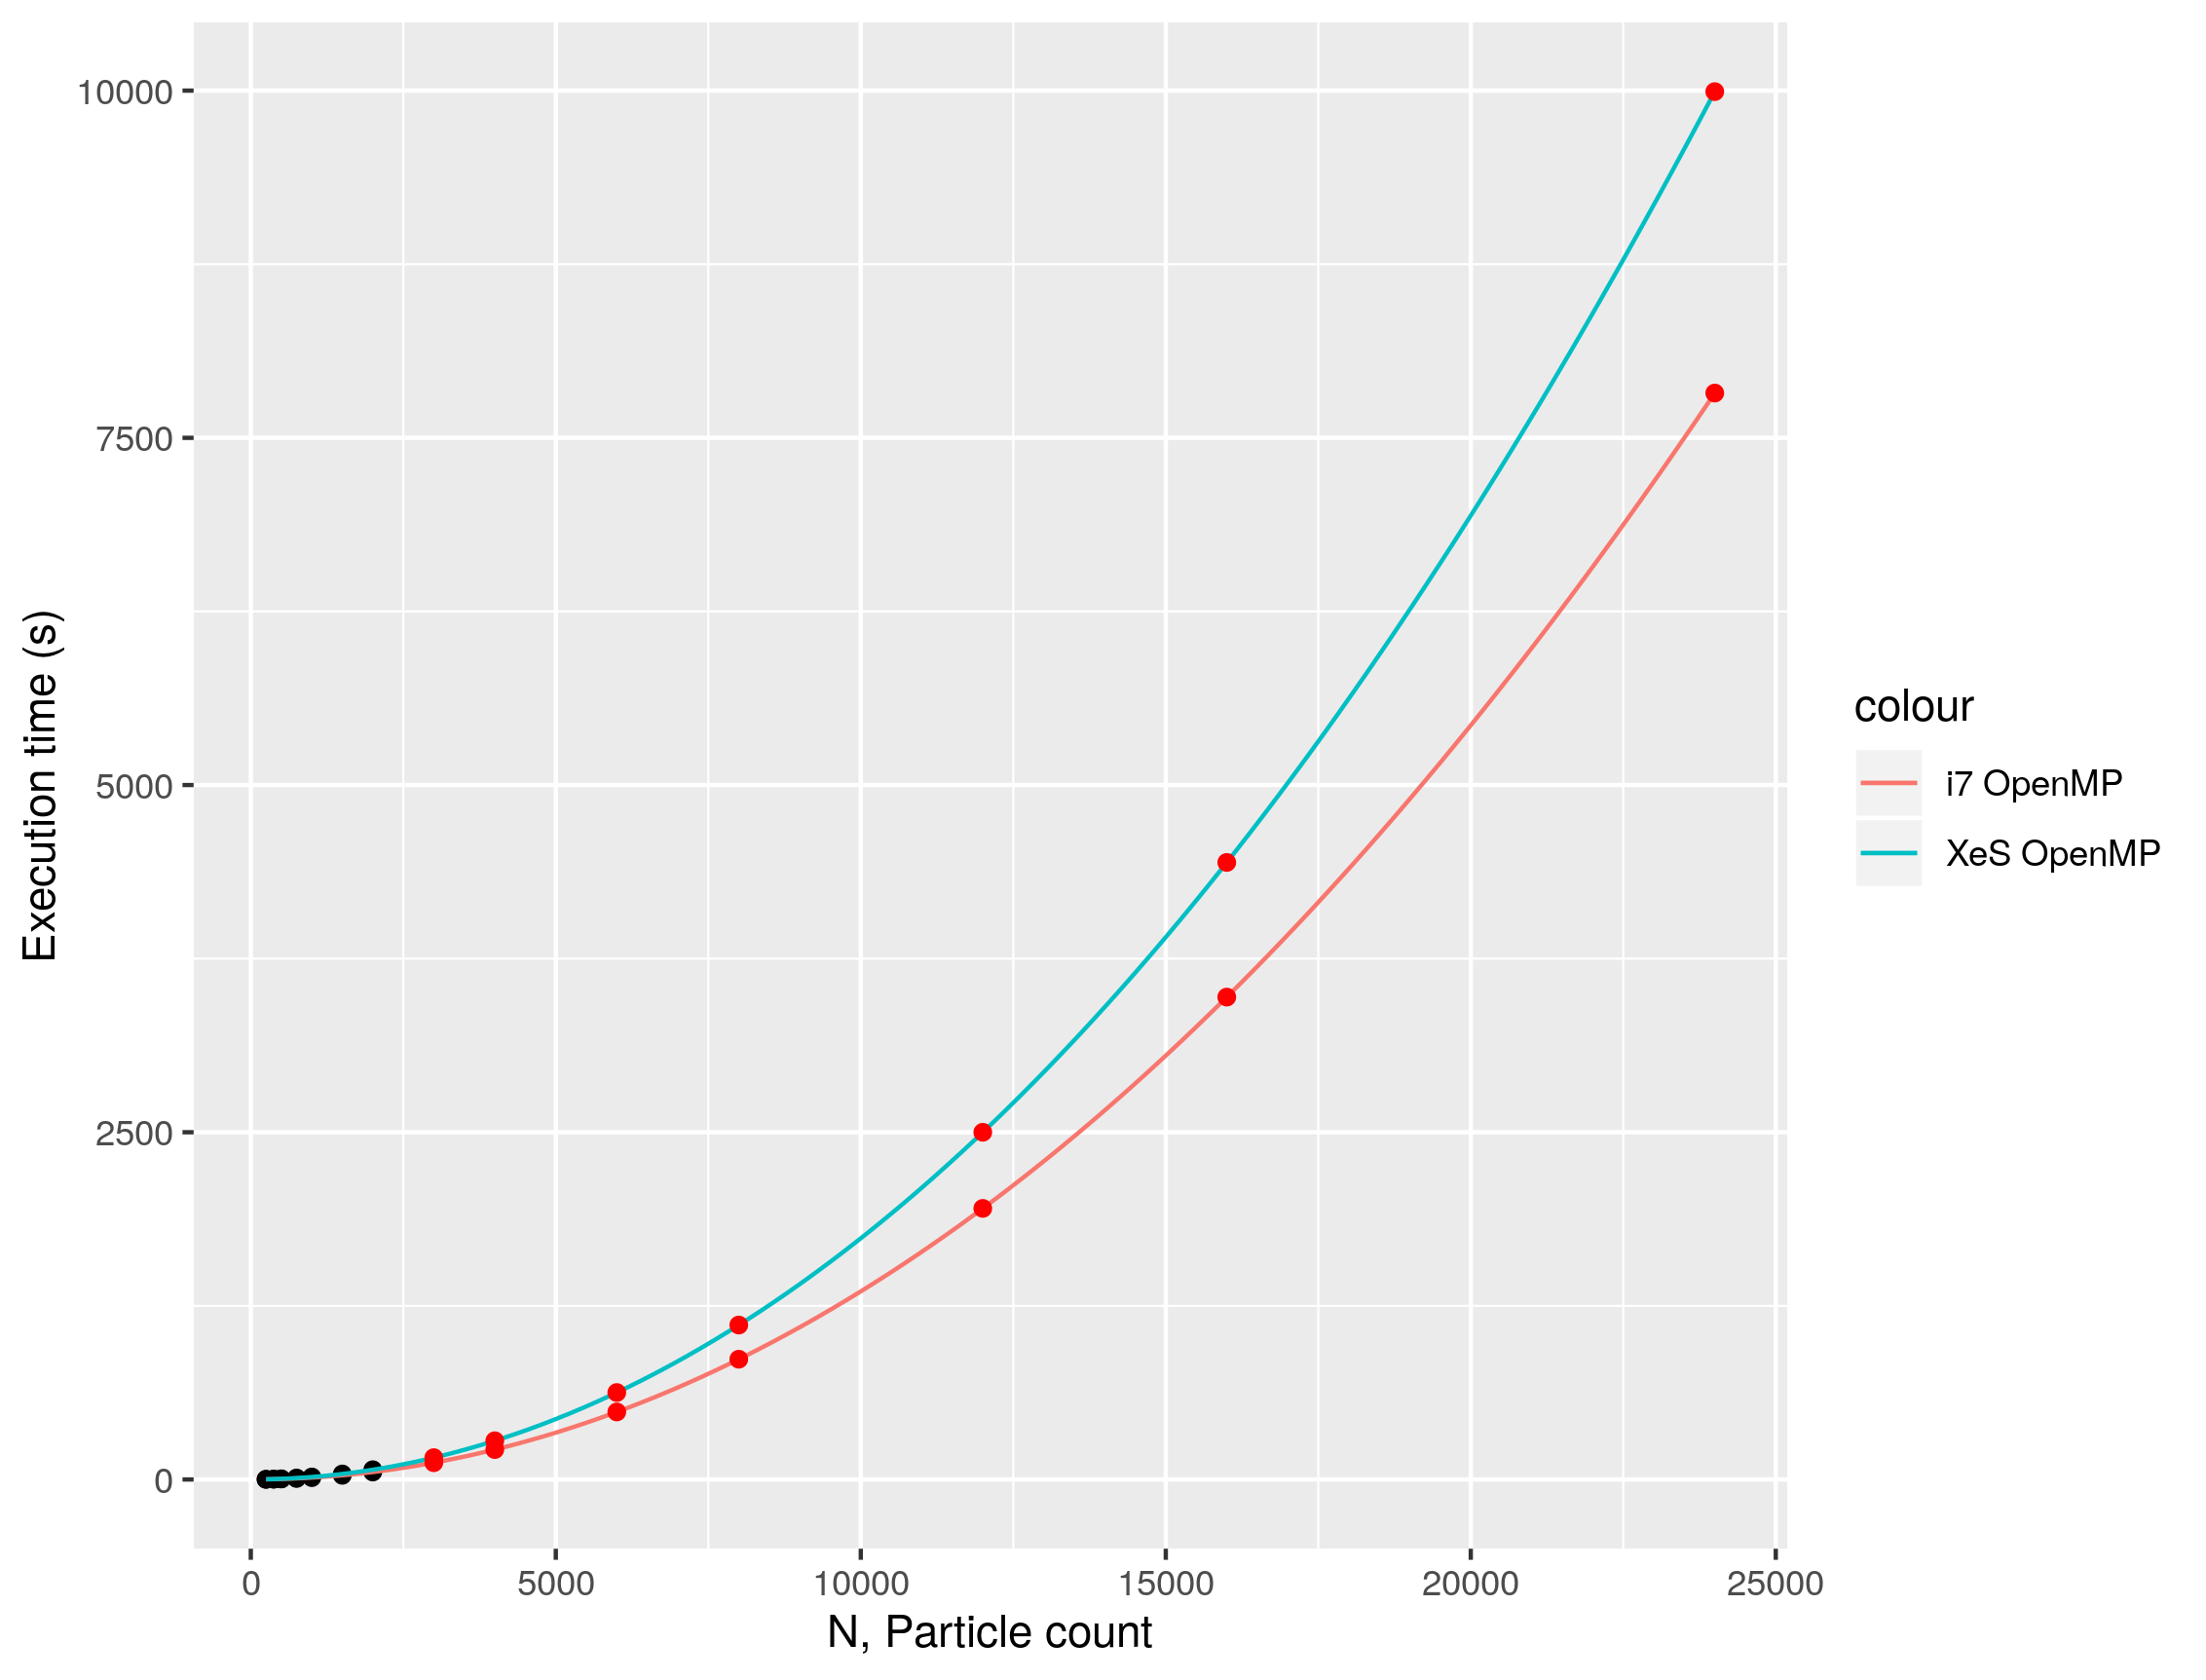
\includegraphics[width=0.8\textwidth]{processedCpuResults/seqExtrapolate.png}
    \caption{Plot of execution time (s) against $N$ (sequential implementation)}
    \label{fig:seqExtrapolate}
\end{figure}

\begin{figure}[H]
    \centering
    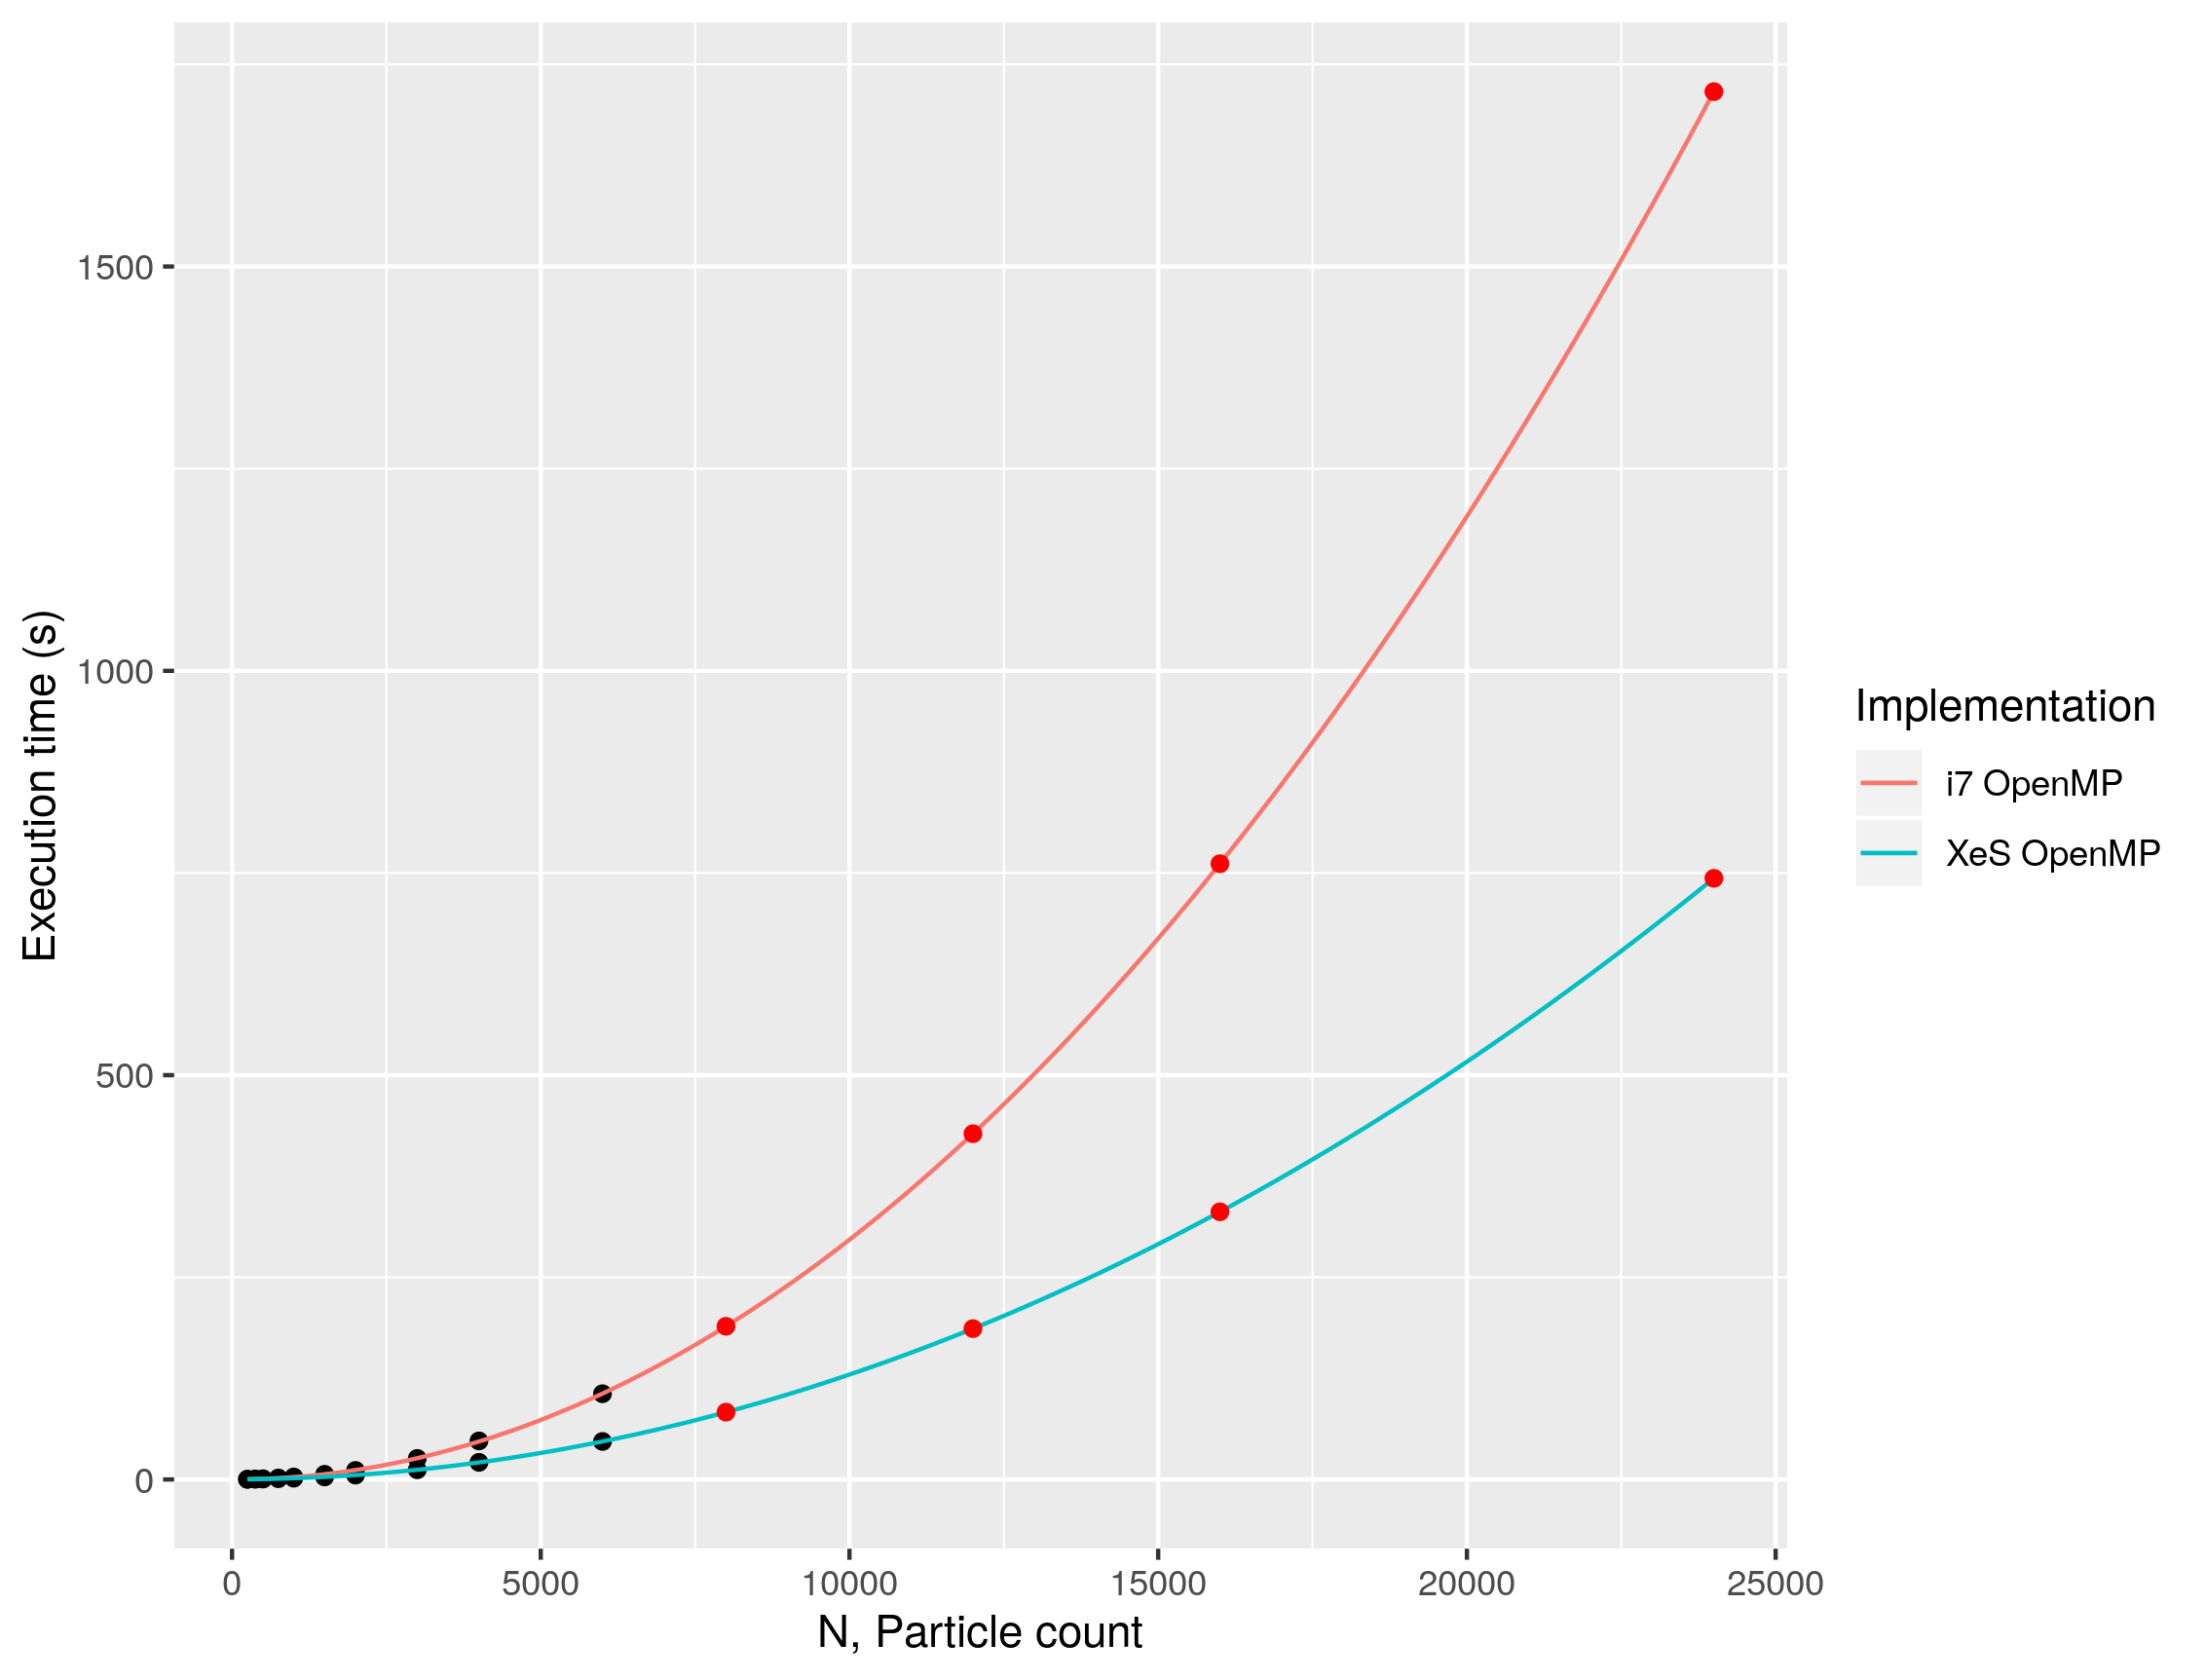
\includegraphics[width=0.8\textwidth]{processedCpuResults/parExtrapolate.png}
    \caption{Plot of execution time (s) against $N$ (OpenMP implementation)}
    \label{fig:parExtrapolate}
\end{figure}

\begin{figure}[H]
    \centering
    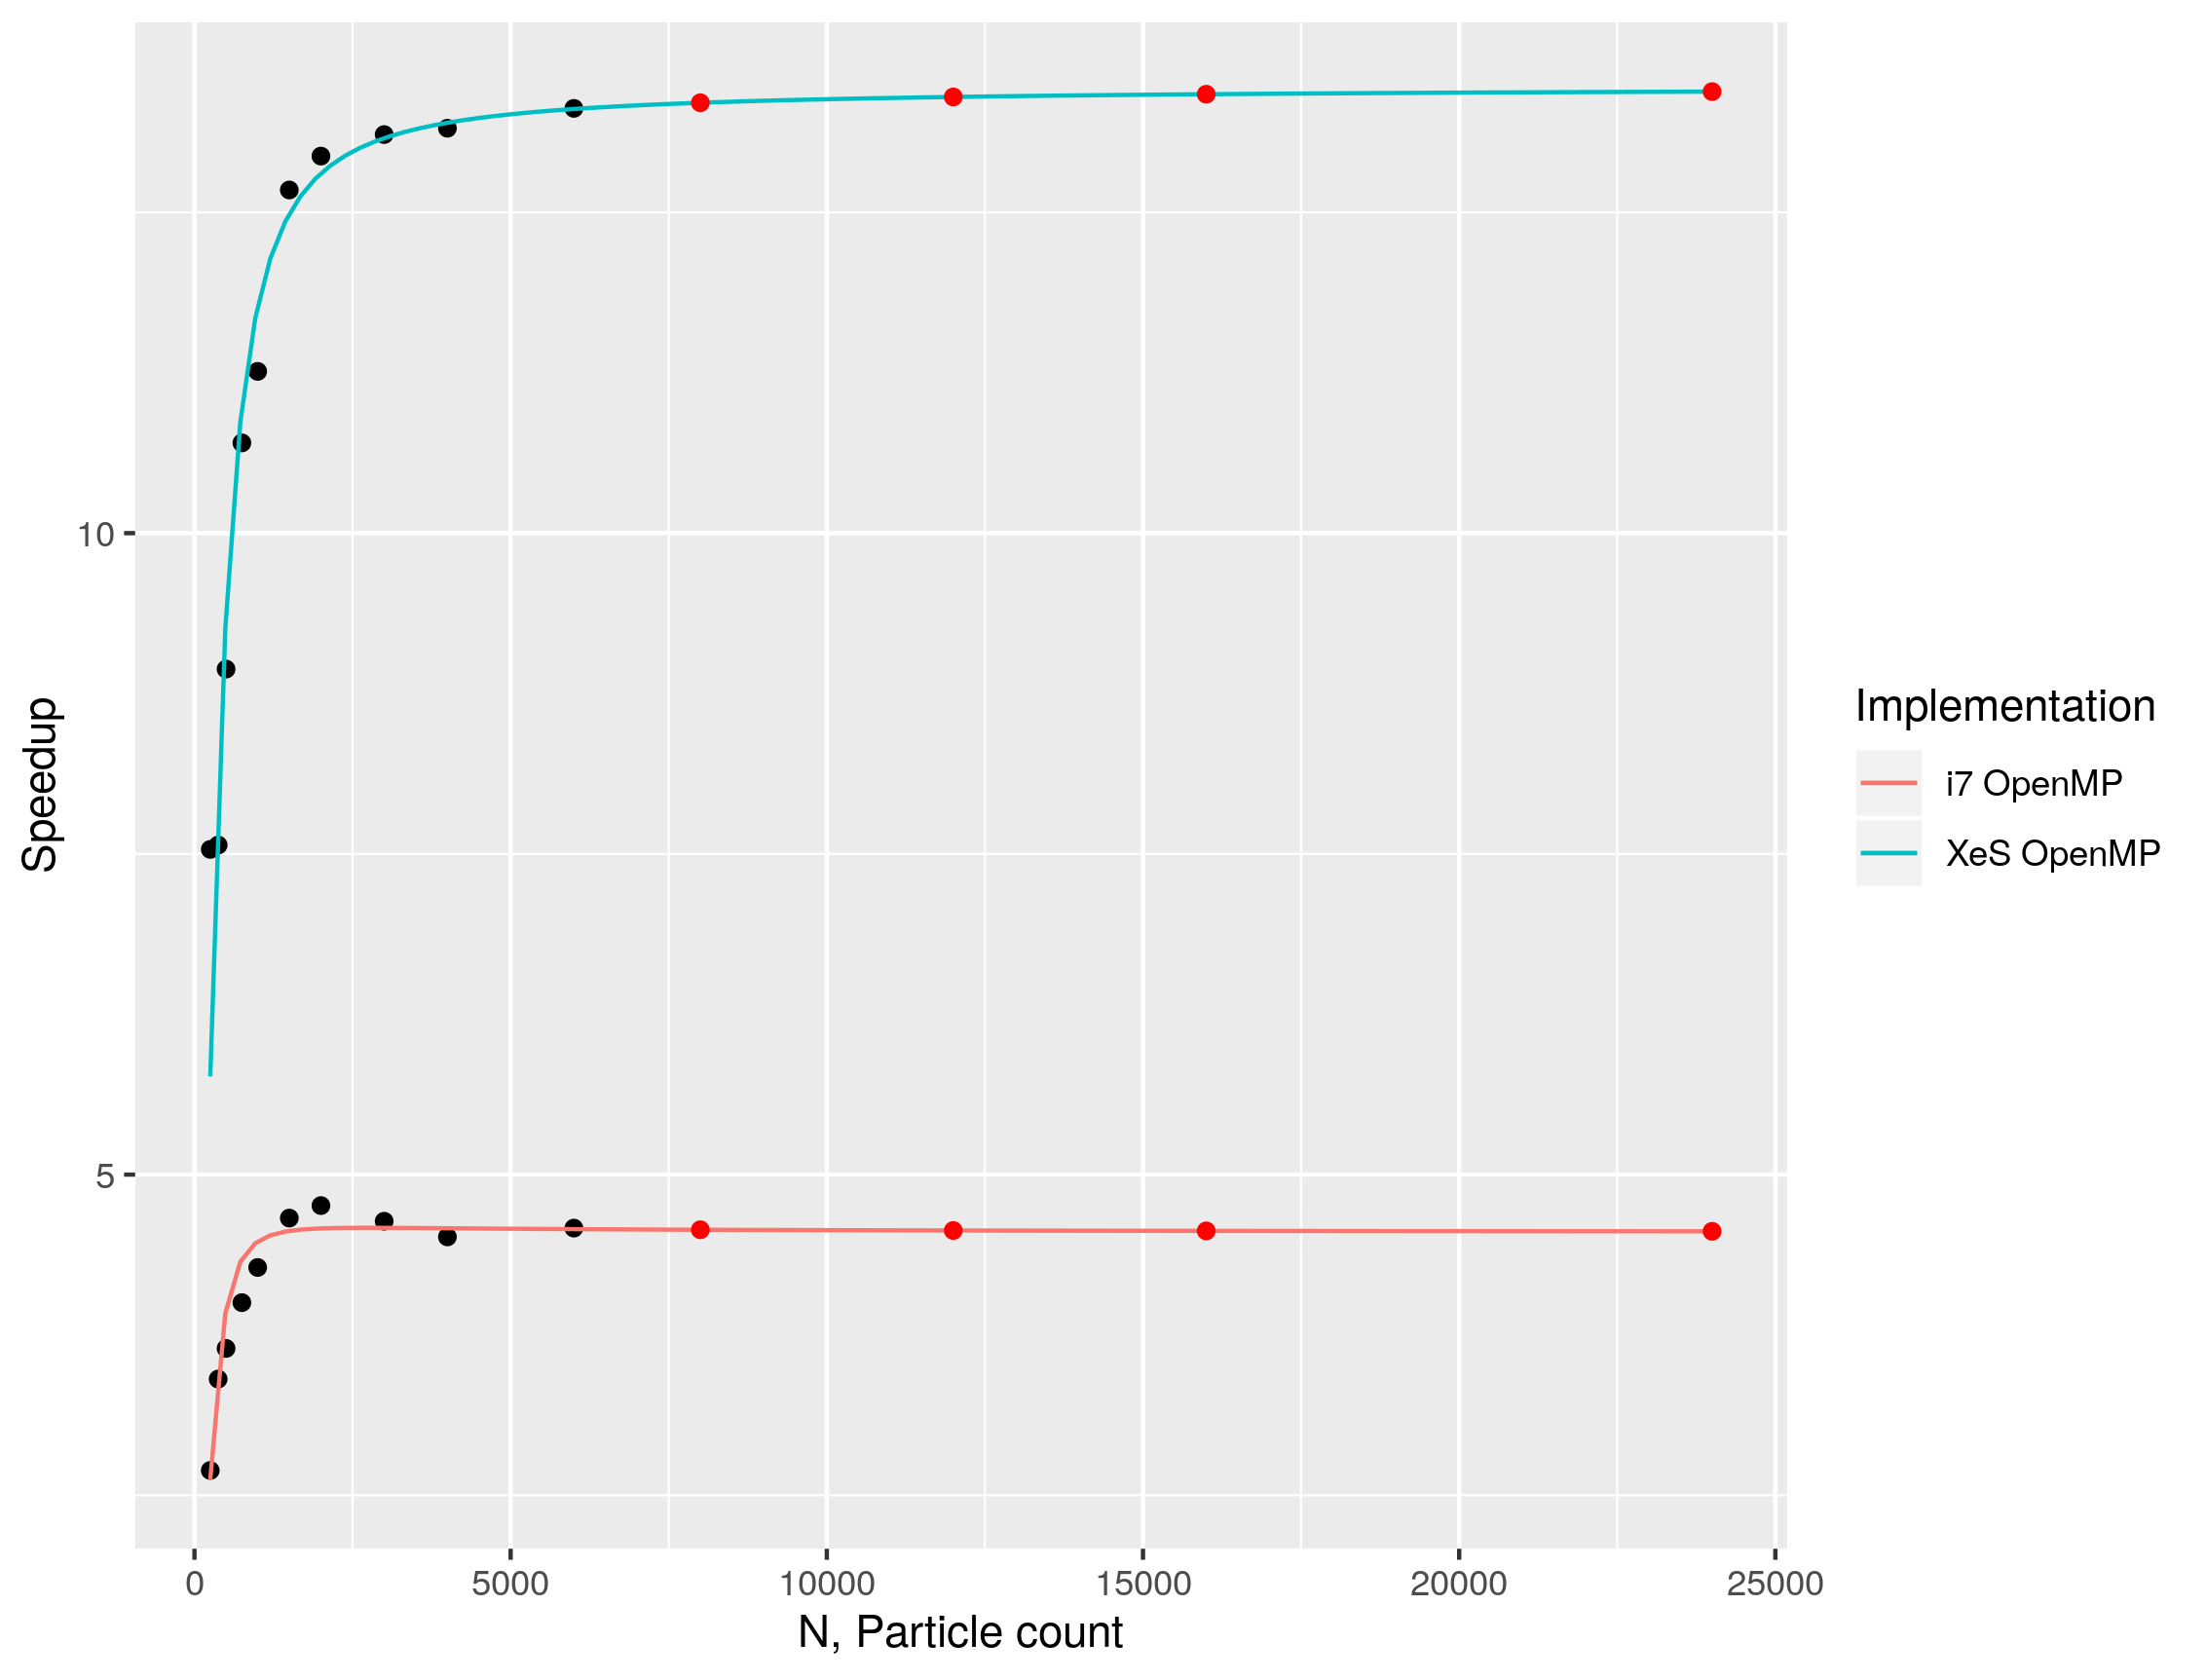
\includegraphics[width=0.8\textwidth]{processedCpuResults/parSpeedupExtrapolate.png}
    \caption{Plot of speedup against $N$ (OpenMP implementation)}
    \label{fig:parSpeedupExtrapolate}
\end{figure}

\subsection{Additional CUDA Results}

\begin{figure}[H]
    \centering
    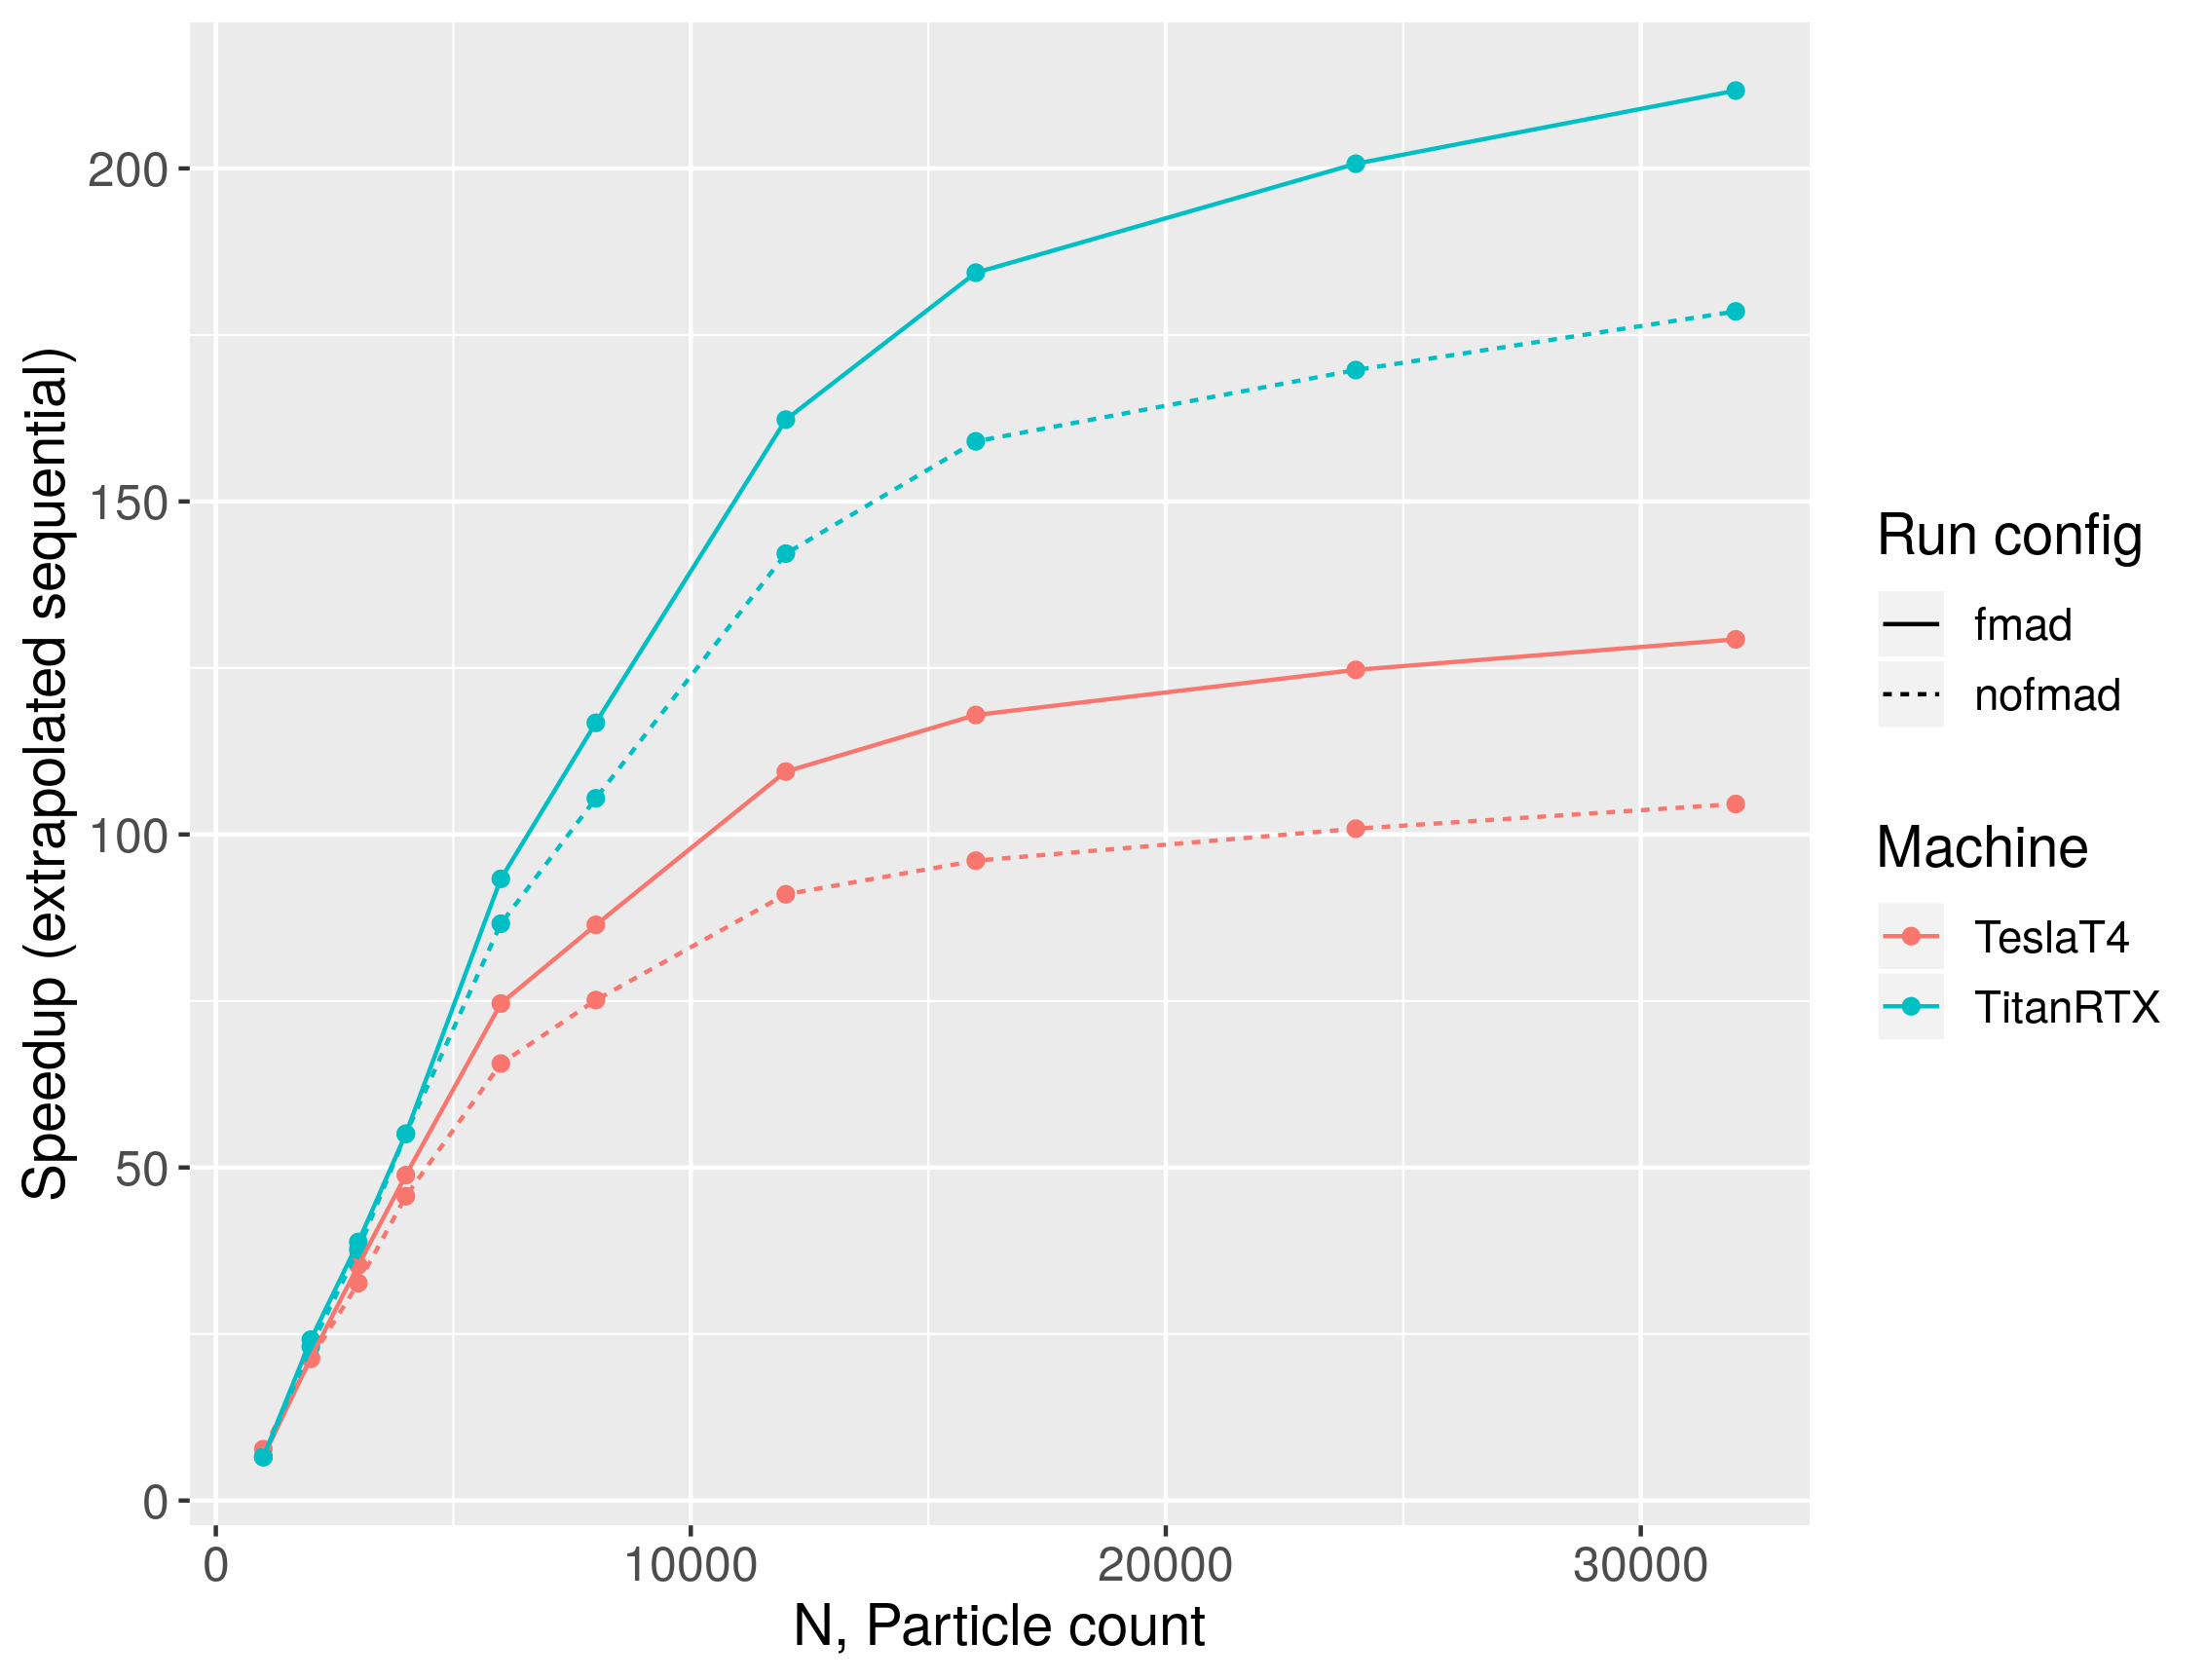
\includegraphics[width=0.75\textwidth]{processedGpuResults/gpu-speedupI7.png}
    \caption{Plot of speedup against $N$ (against i7-7700K sequential results)}
    \label{fig:gpu-speedupI7}
\end{figure}

\begin{figure}[H]
    \centering
    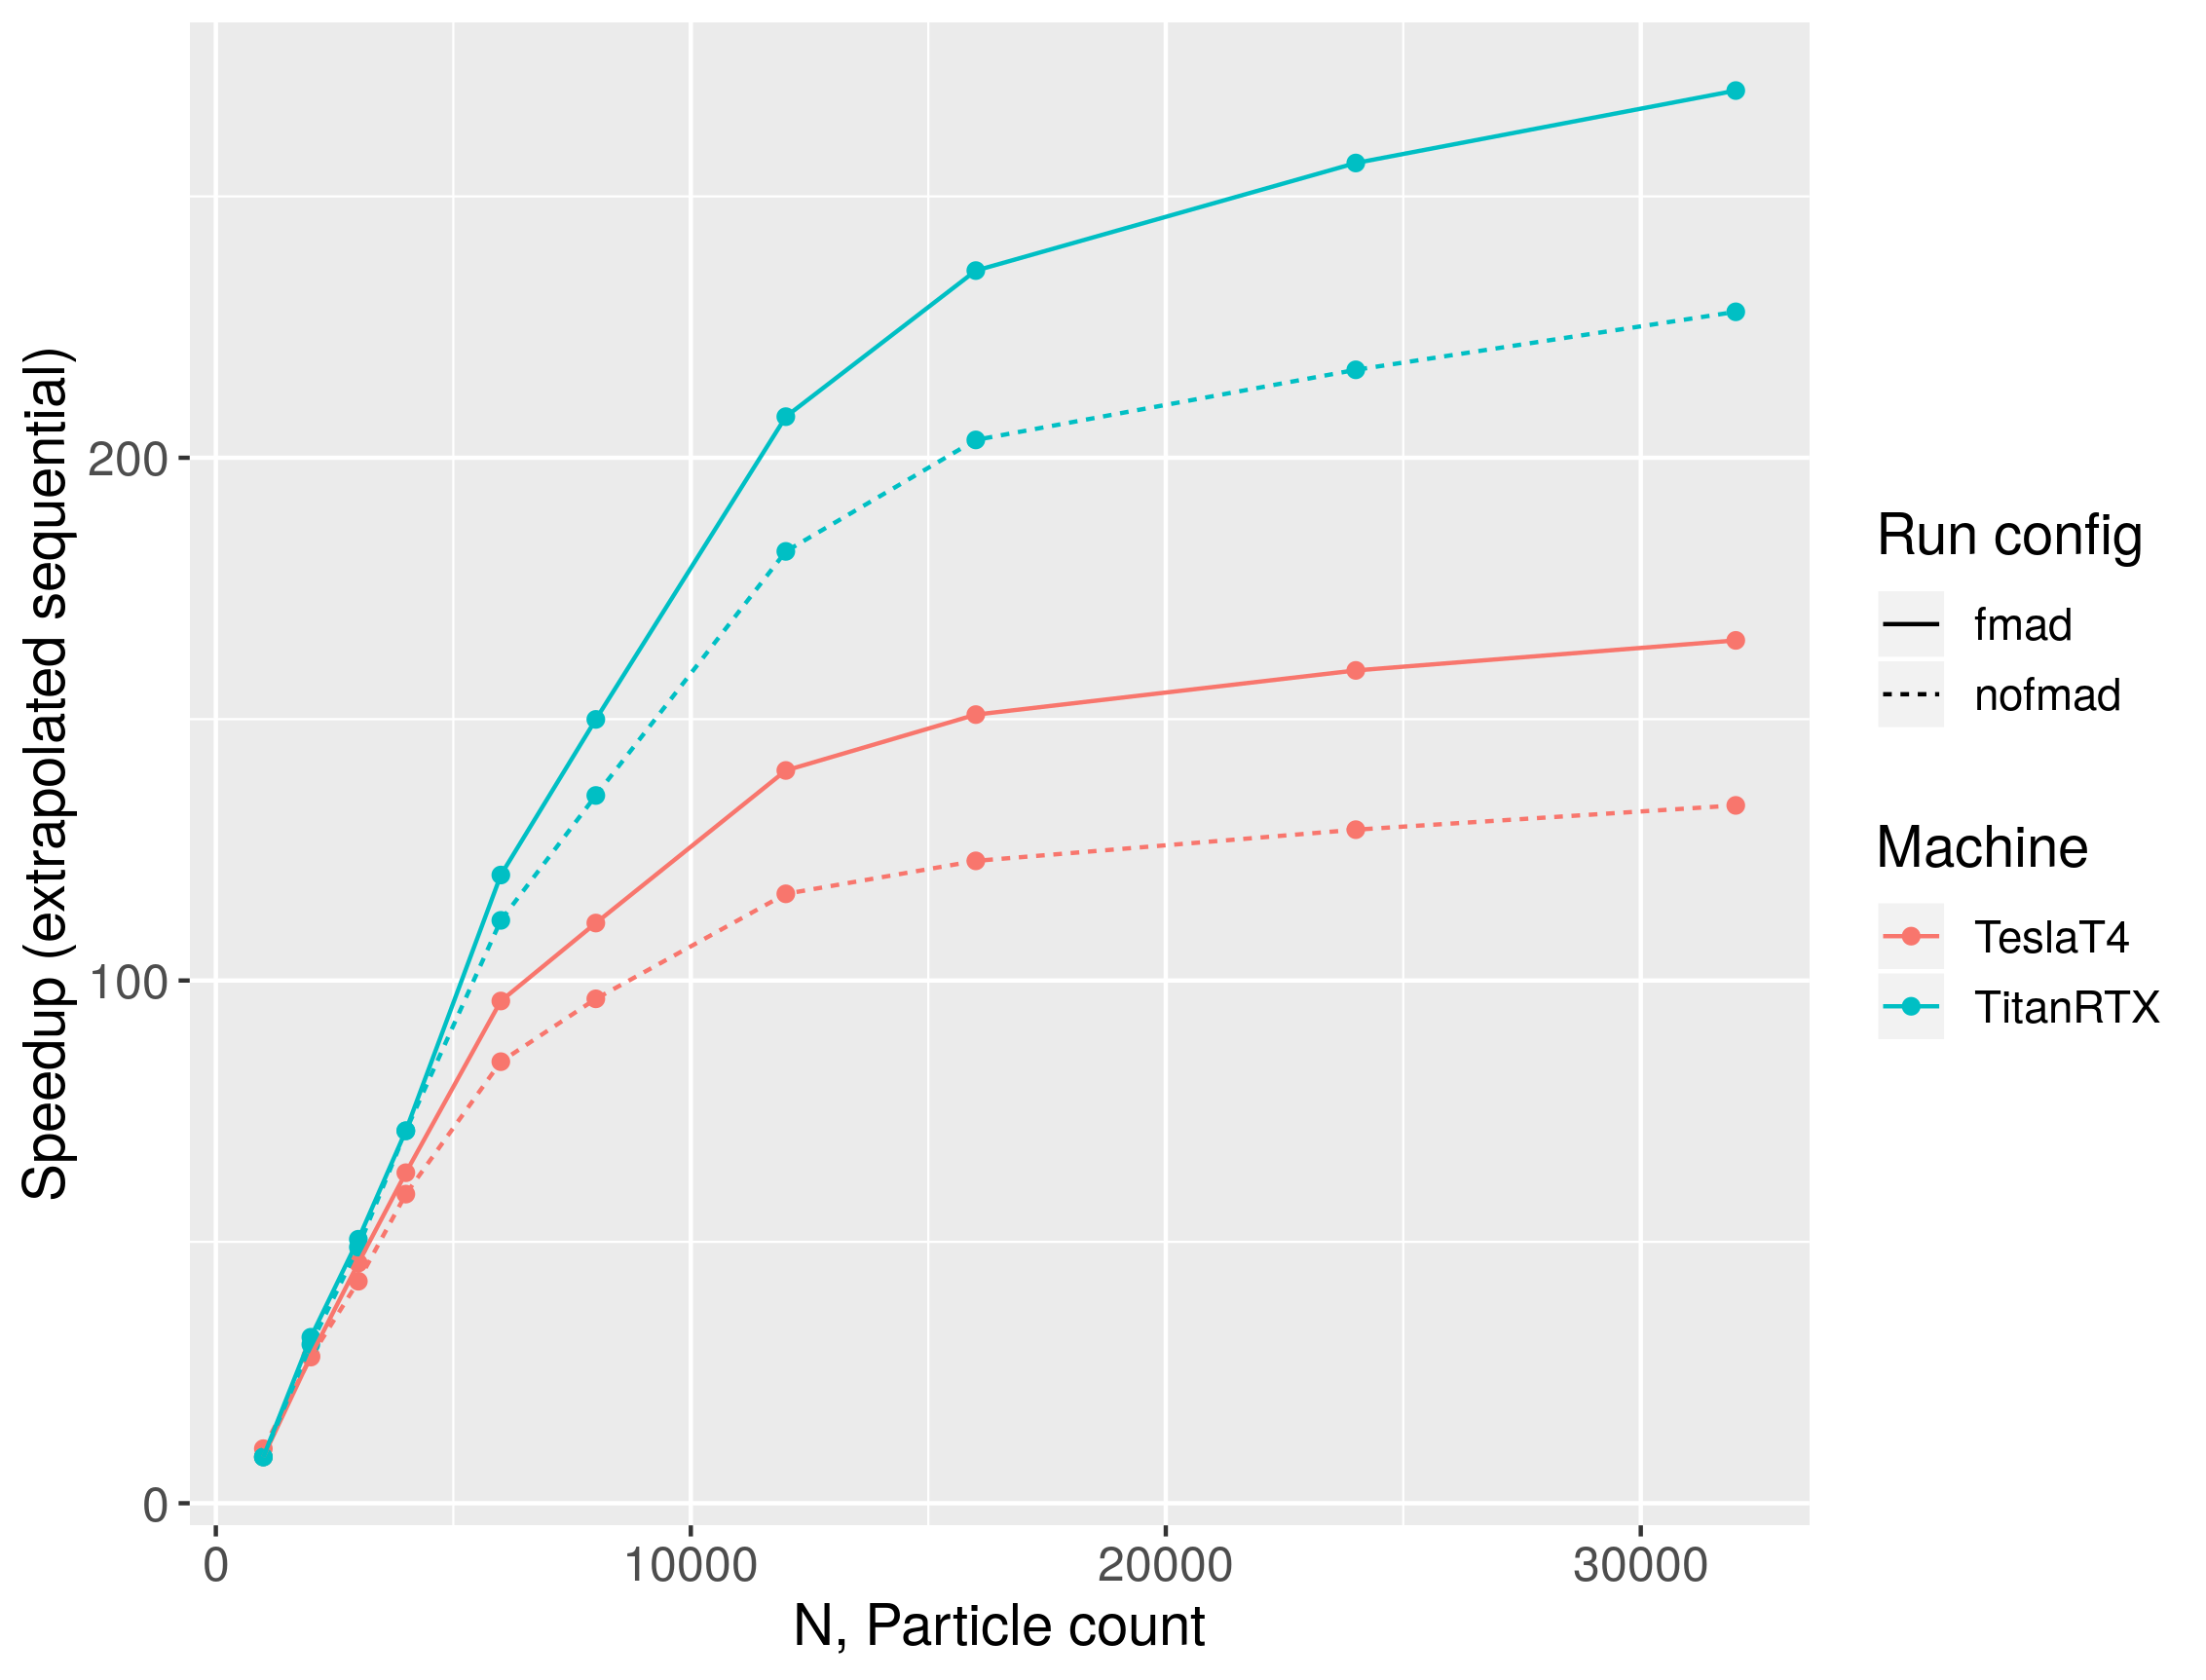
\includegraphics[width=0.75\textwidth]{processedGpuResults/gpu-speedupXeS.png}
    \caption{Plot of speedup against $N$ (against Xeon 4114 sequential results)}
    \label{fig:gpu-speedupXeS}
\end{figure}

\subsection{MPI Results (Xeon 4114 configuration)}

\begin{figure}[H]
    \centering
    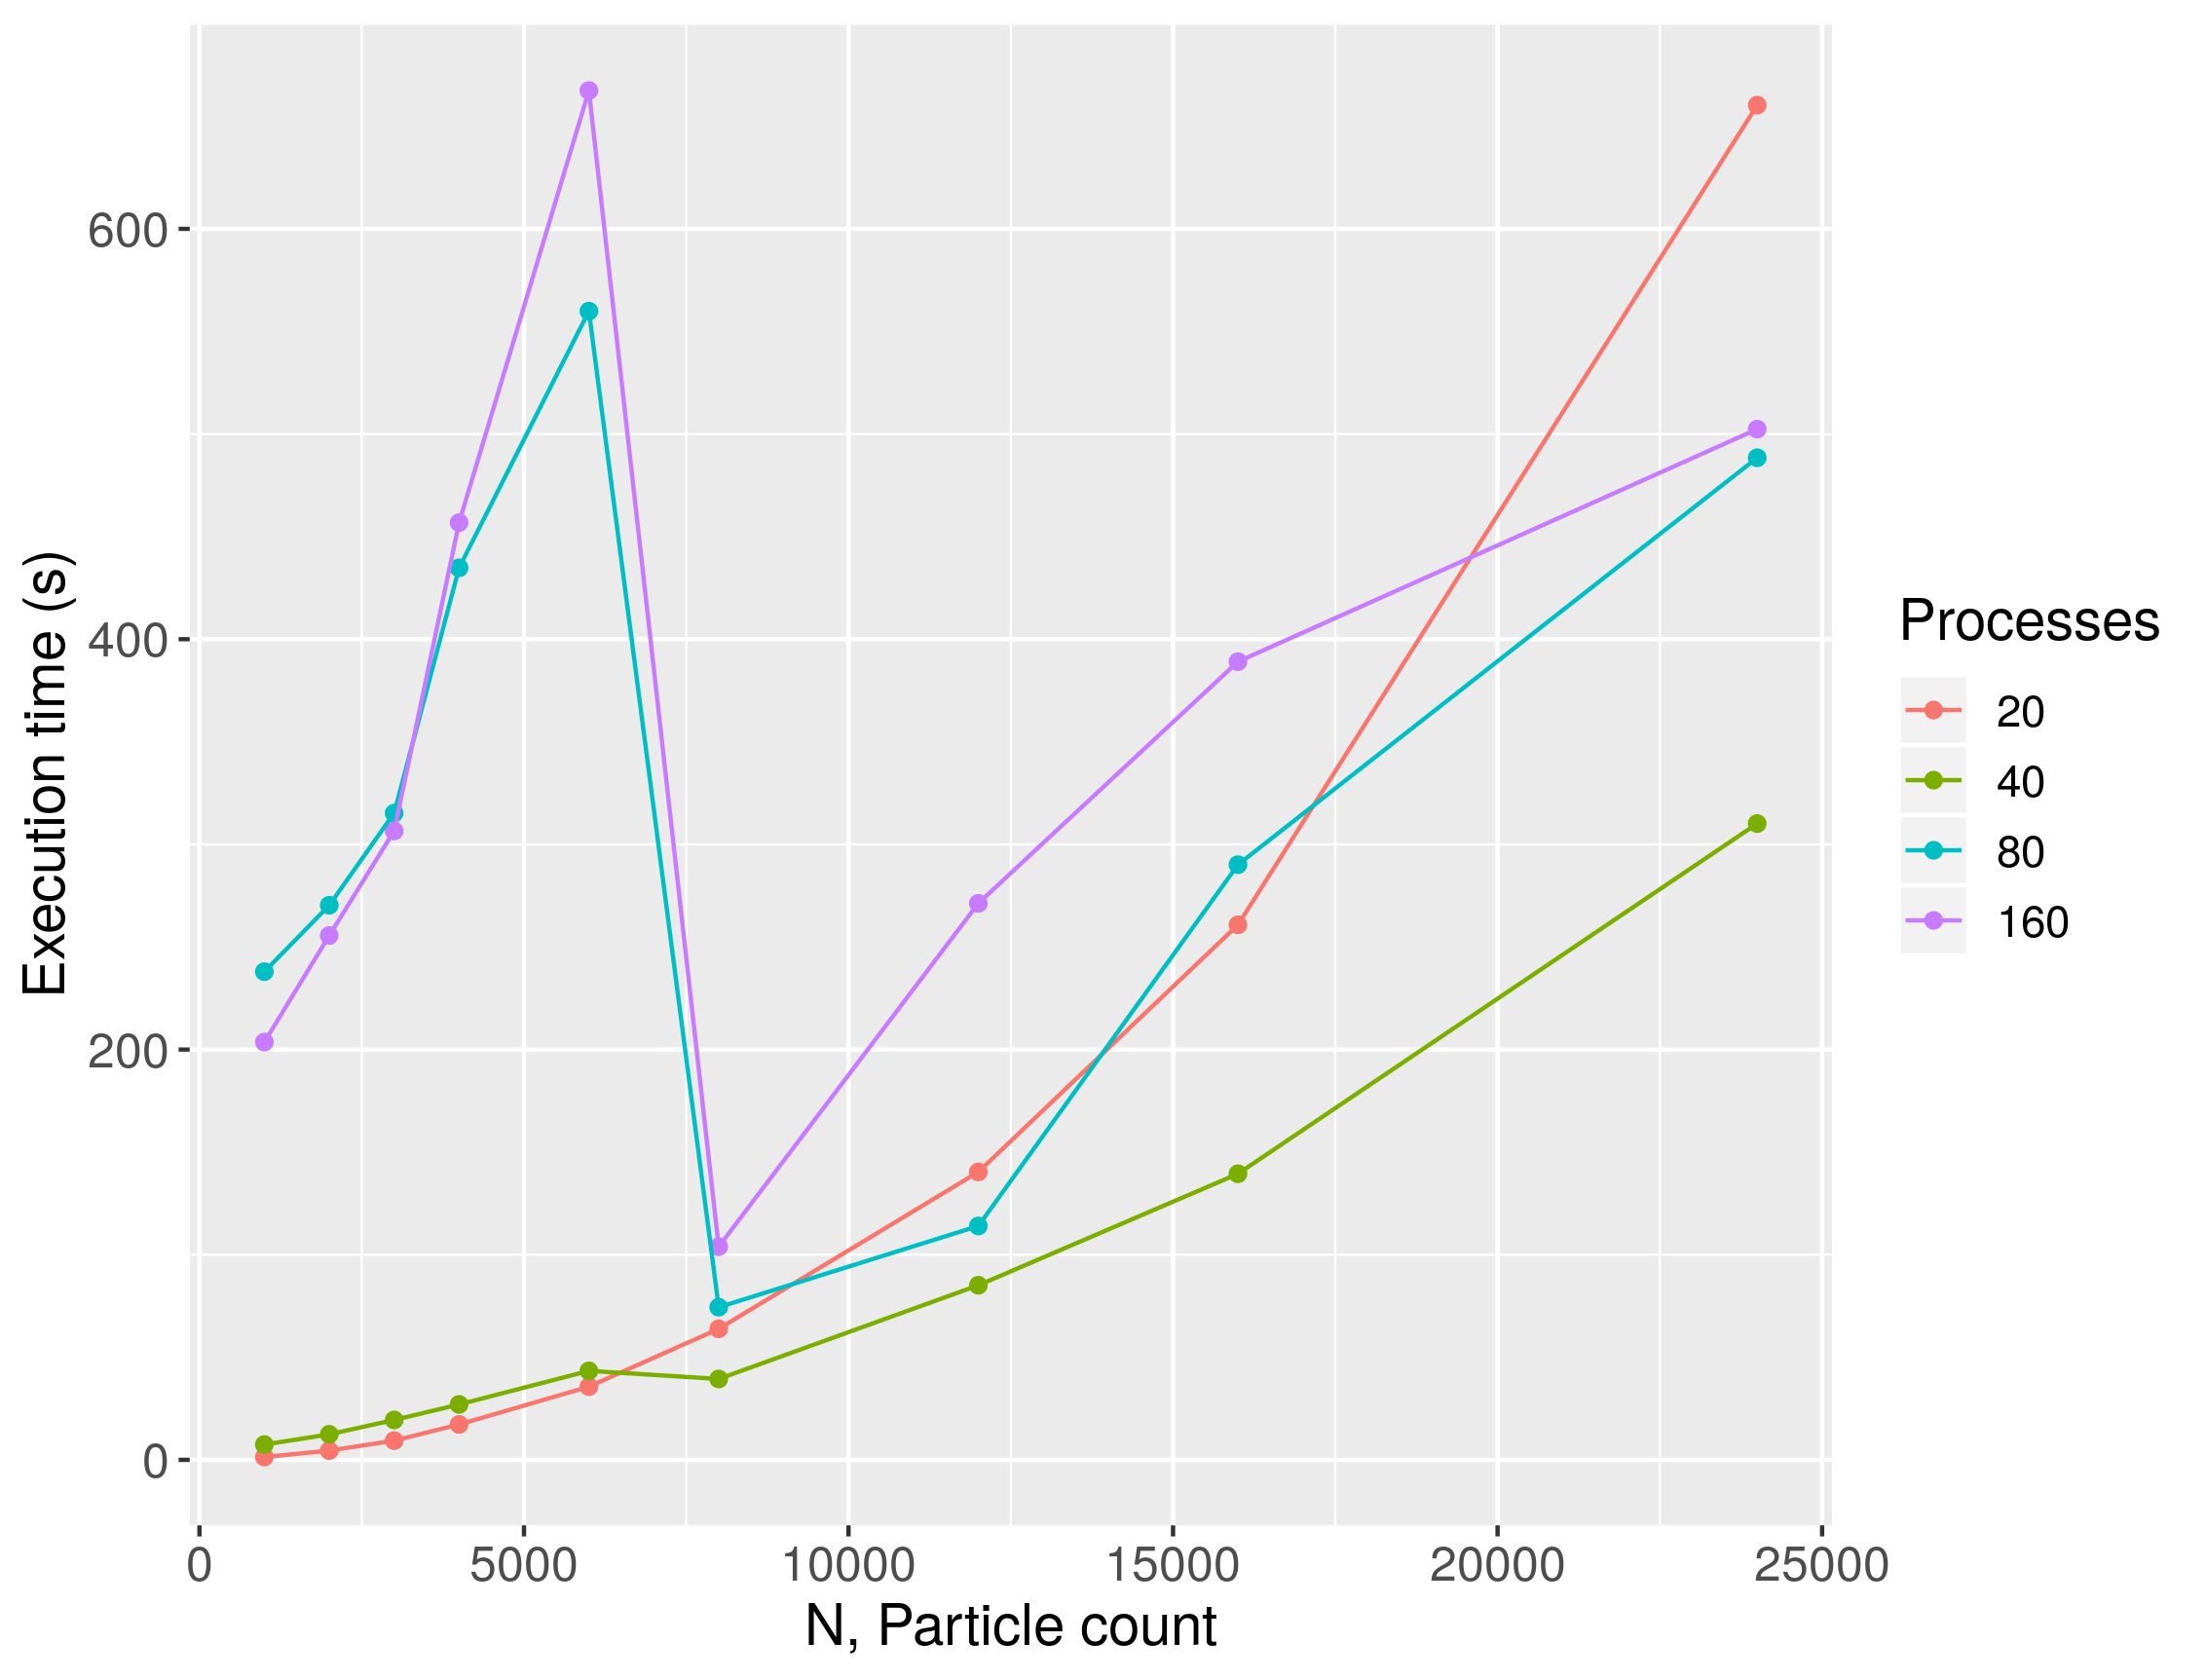
\includegraphics[width=0.74\textwidth]{processedCpuResults/PureXeS-varyNandProcesses.png}
    \caption{Plot of execution time (s) against $N$ for varying processes (Xeon 4114 configuration)}
    \label{fig:PureXeS-varyNandProcesses}
\end{figure}

\begin{figure}[H]
    \centering
    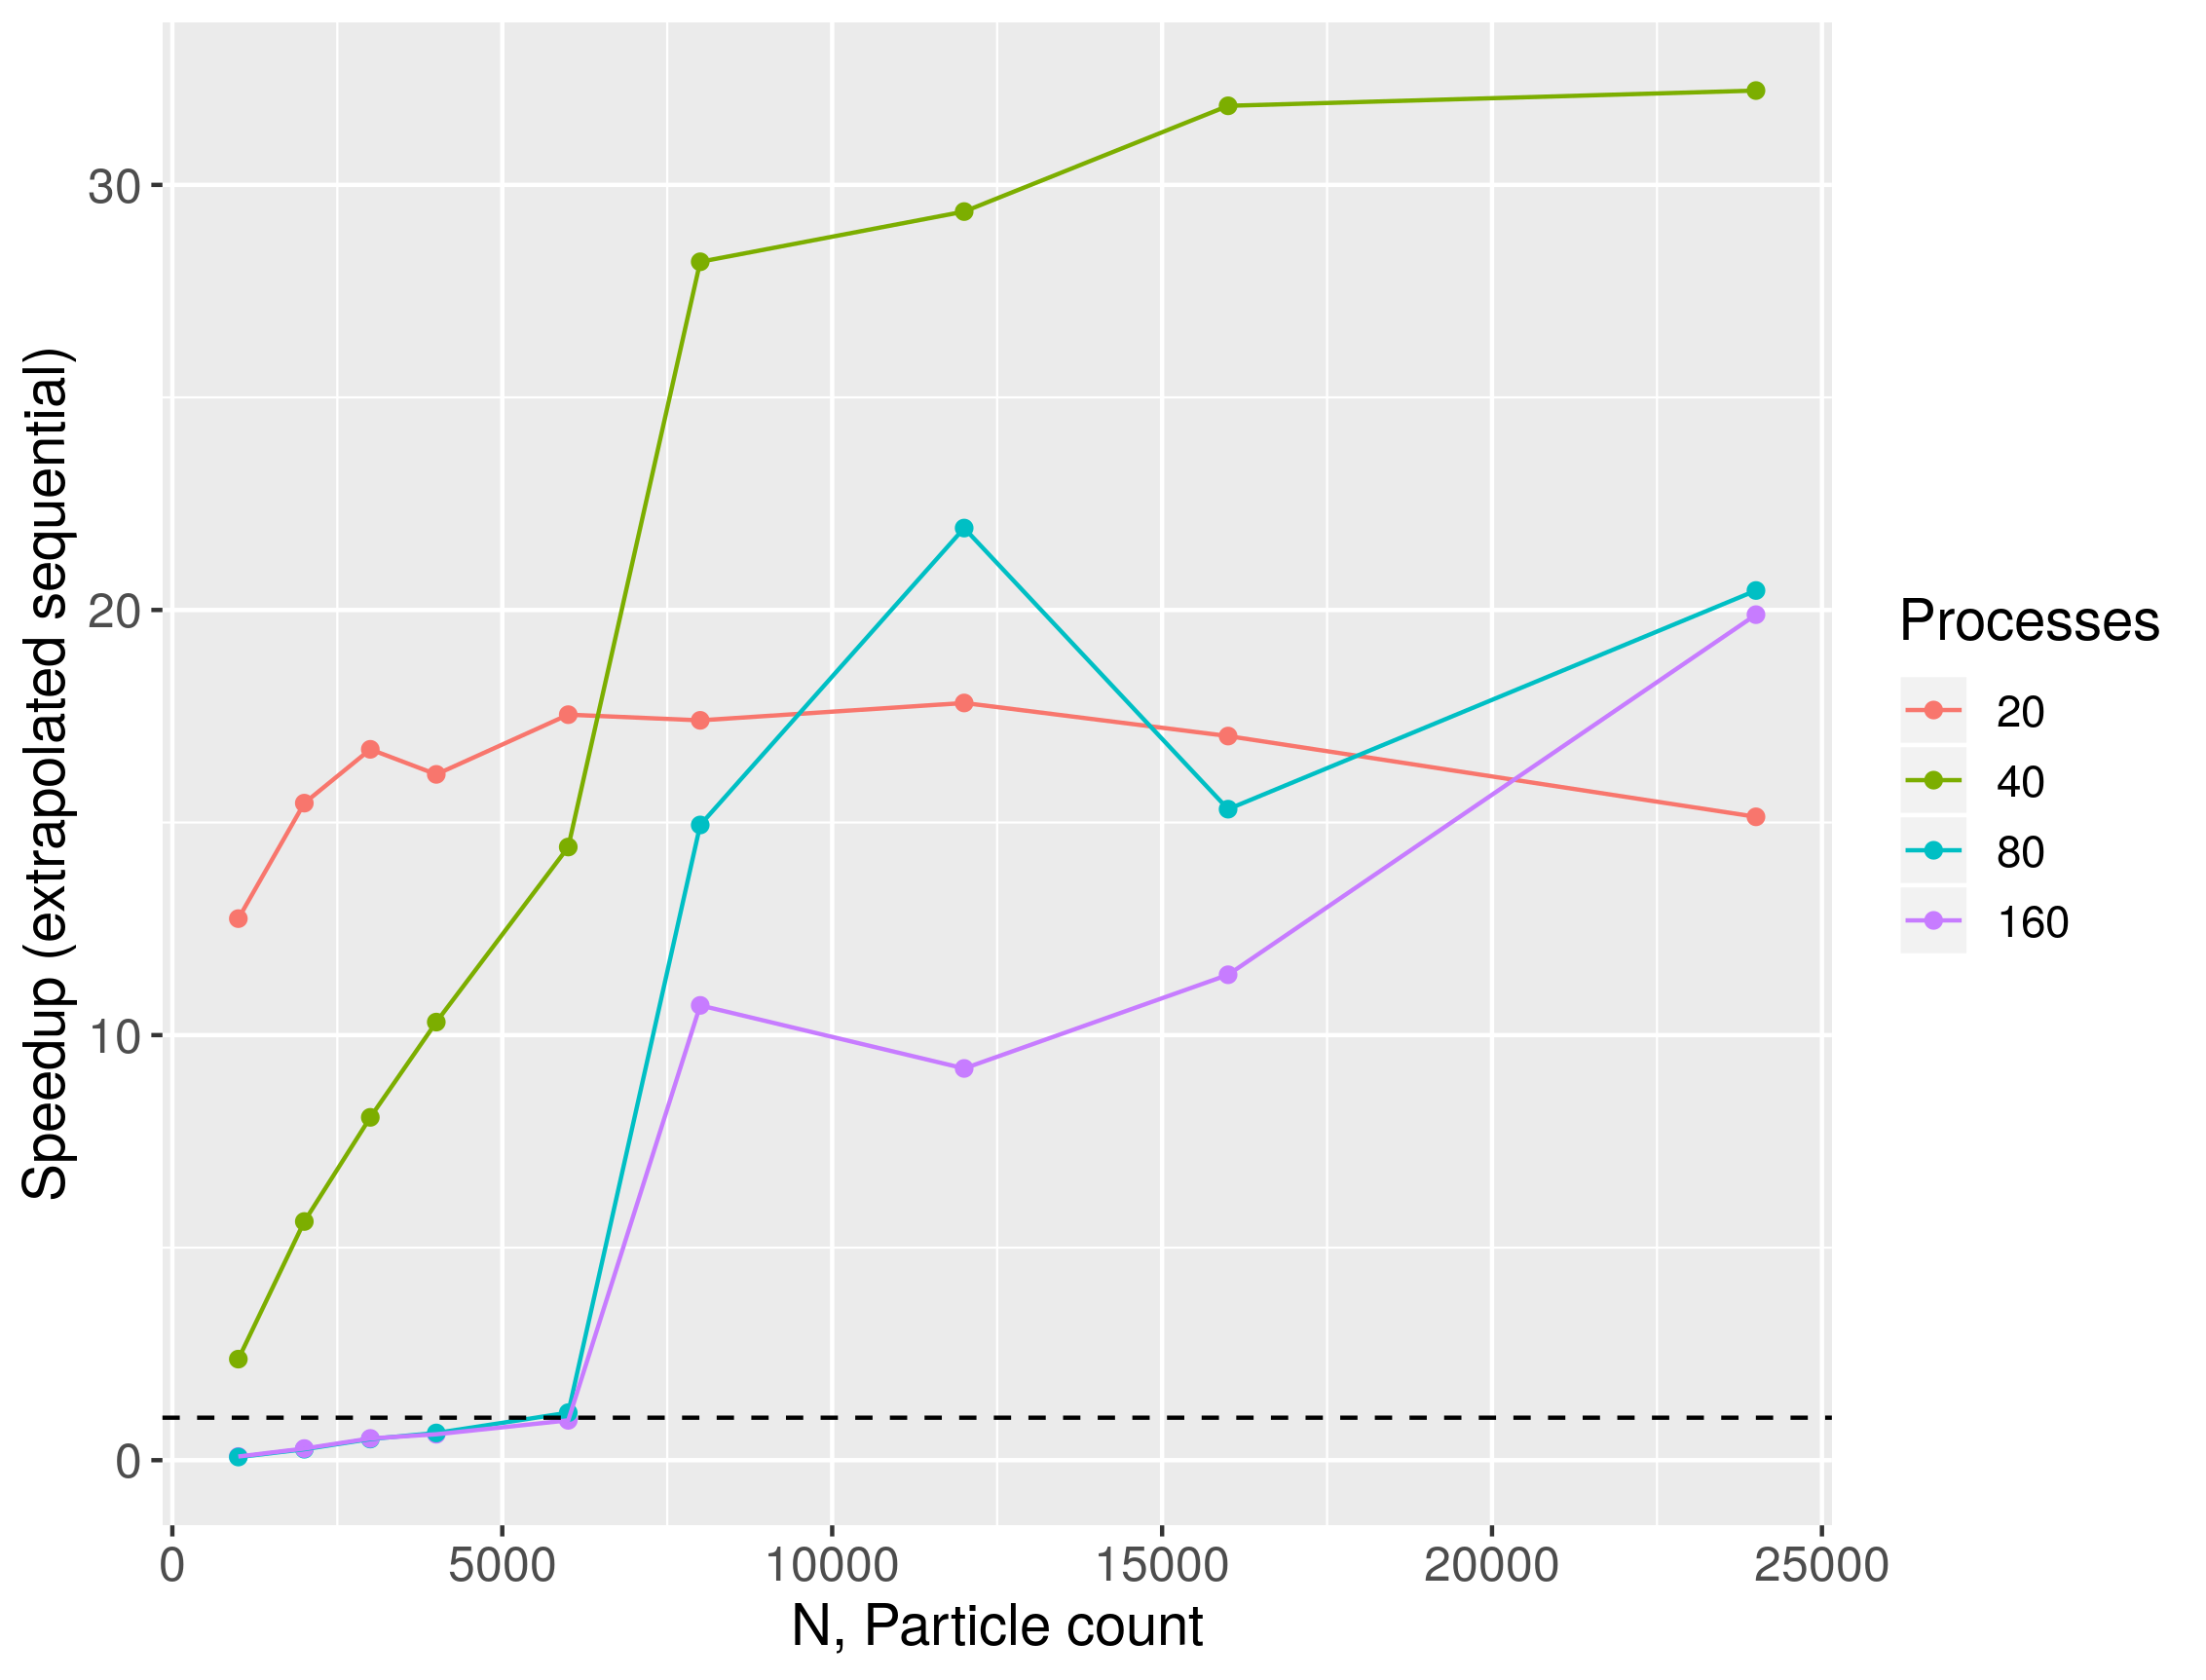
\includegraphics[width=0.74\textwidth]{processedCpuResults/PureXeS-seqSpeedup.png}
    \caption{Plot of speedup against $N$ for varying processes (Xeon 4114 configuration)}
    \label{fig:PureXeS-seqSpeedup}
\end{figure}

\subsection{MPI Results (i7-7700K configuration)}

\begin{figure}[H]
    \centering
    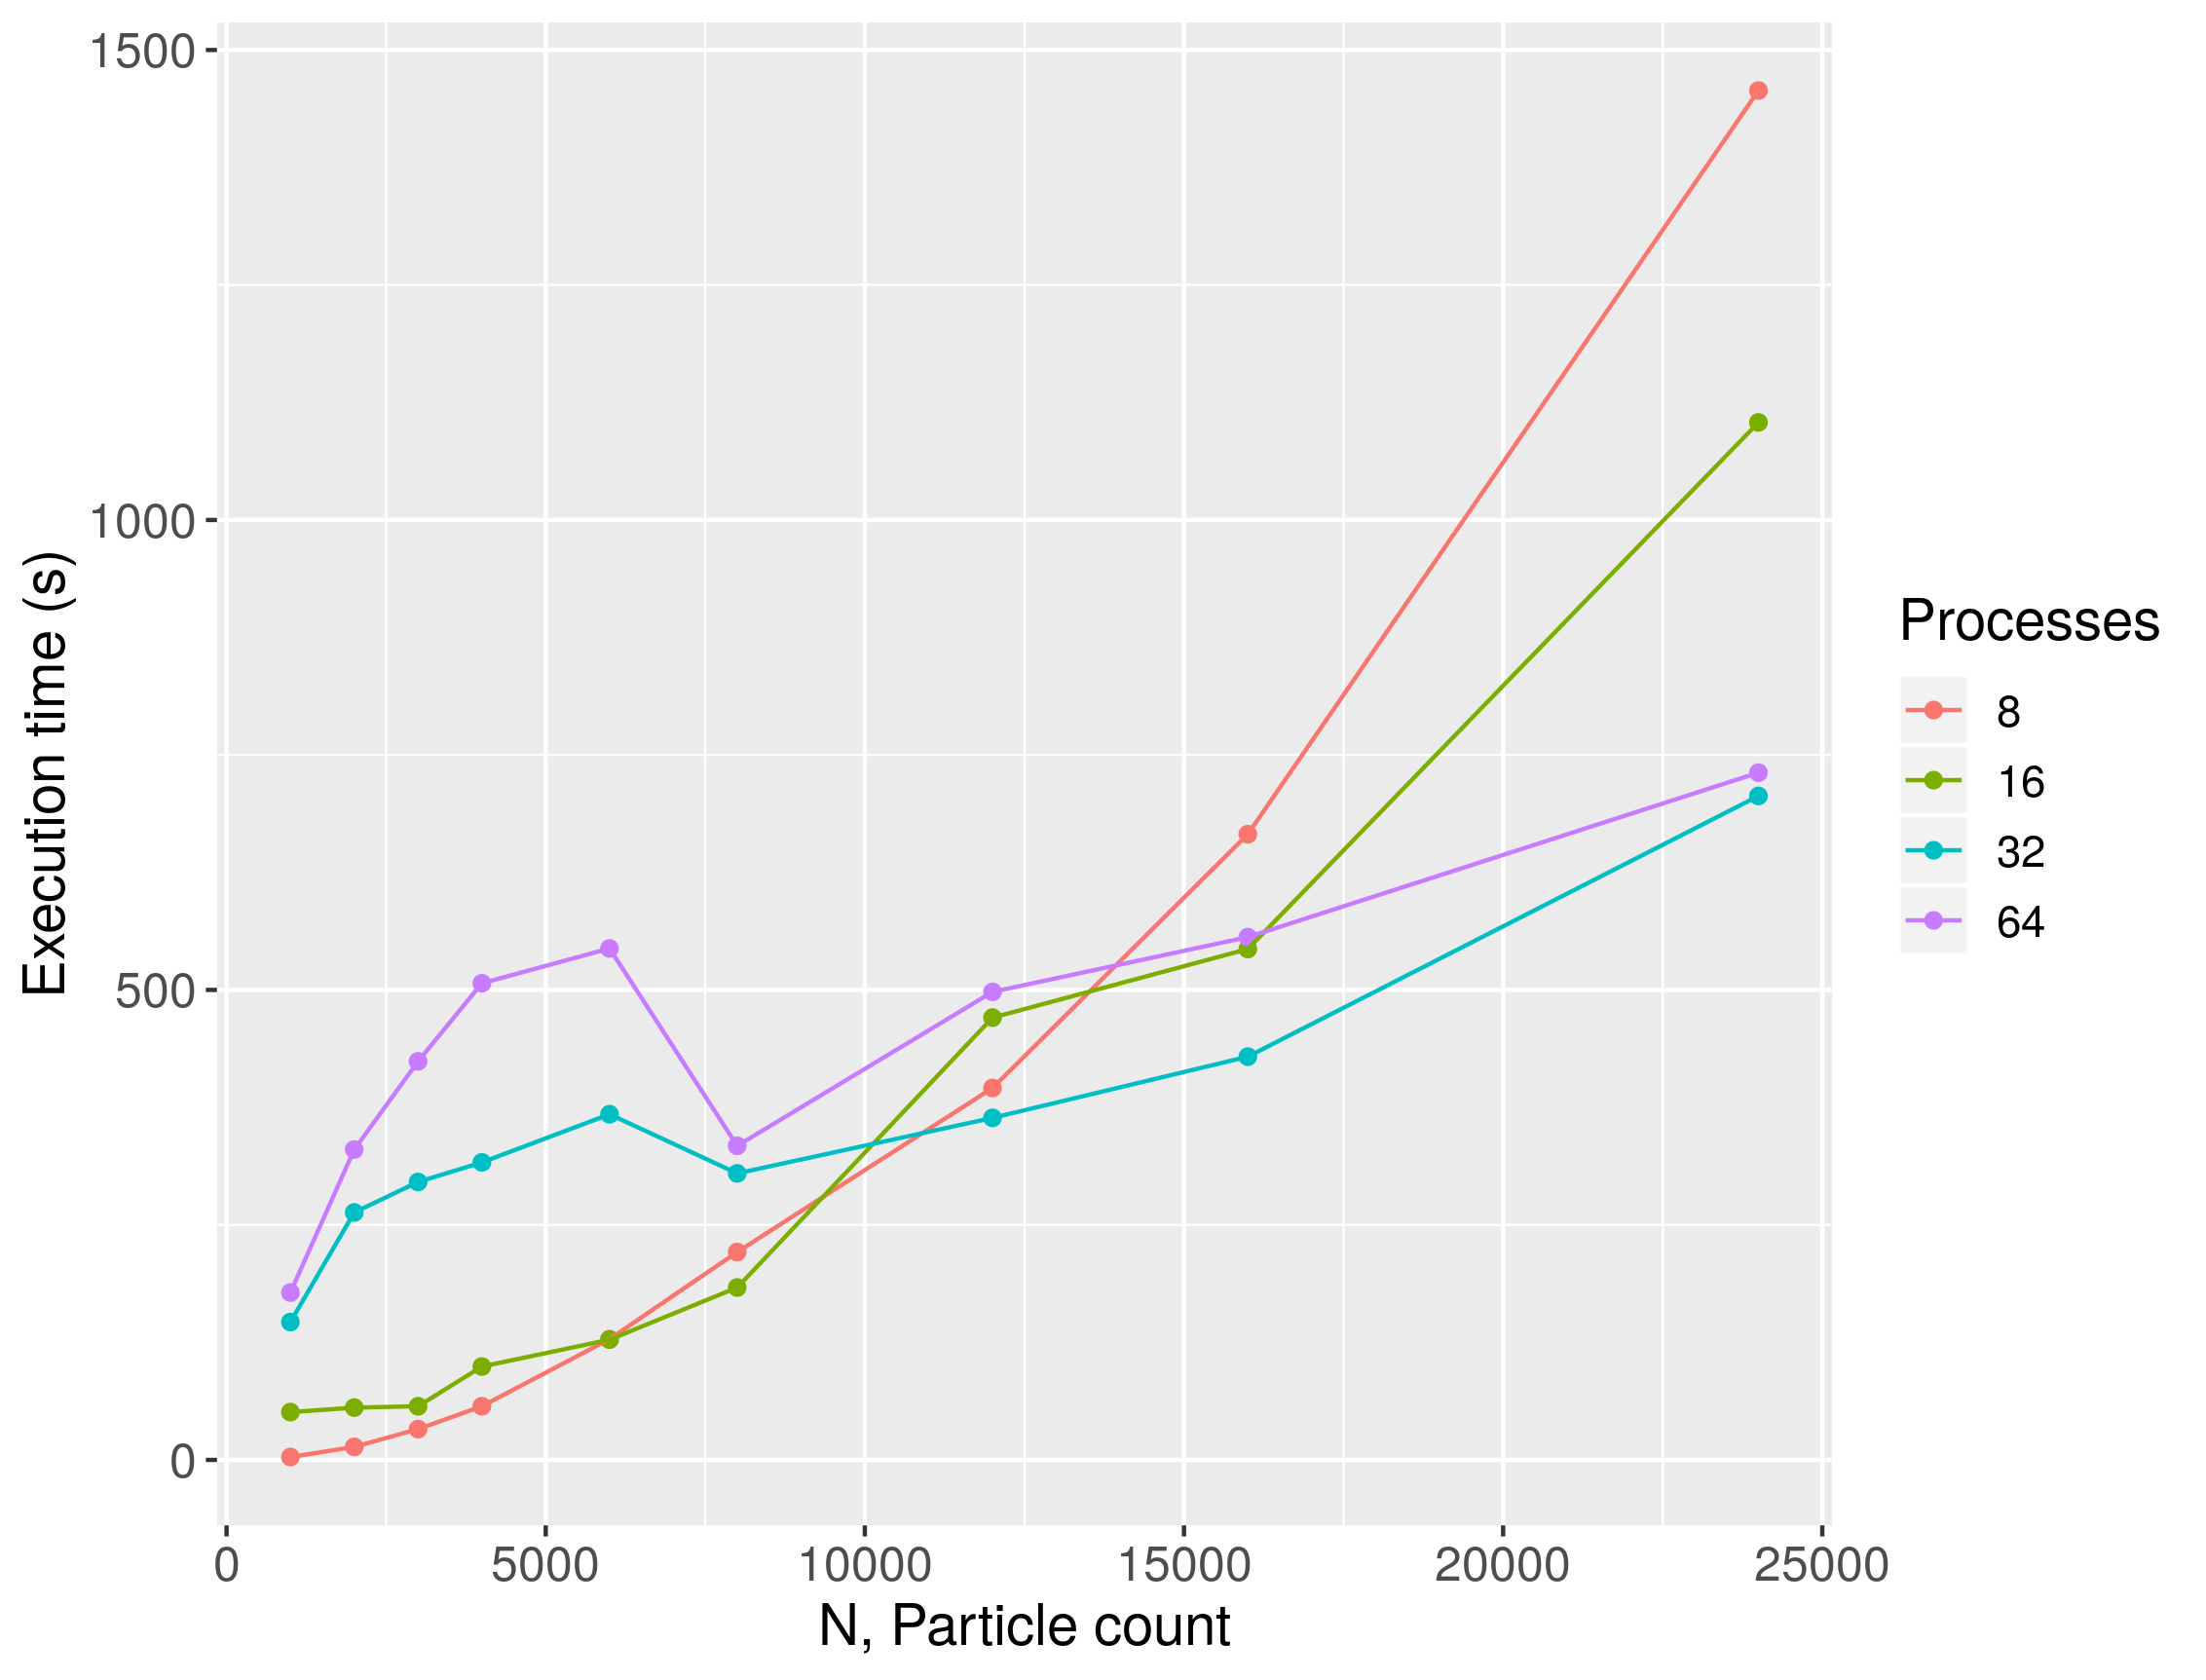
\includegraphics[width=0.74\textwidth]{processedCpuResults/PureI7-varyNandProcesses.png}
    \caption{Plot of execution time (s) against $N$ for varying processes (i7-7700K configuration)}
    \label{fig:PureI7-varyNandProcesses}
\end{figure}

\begin{figure}[H]
    \centering
    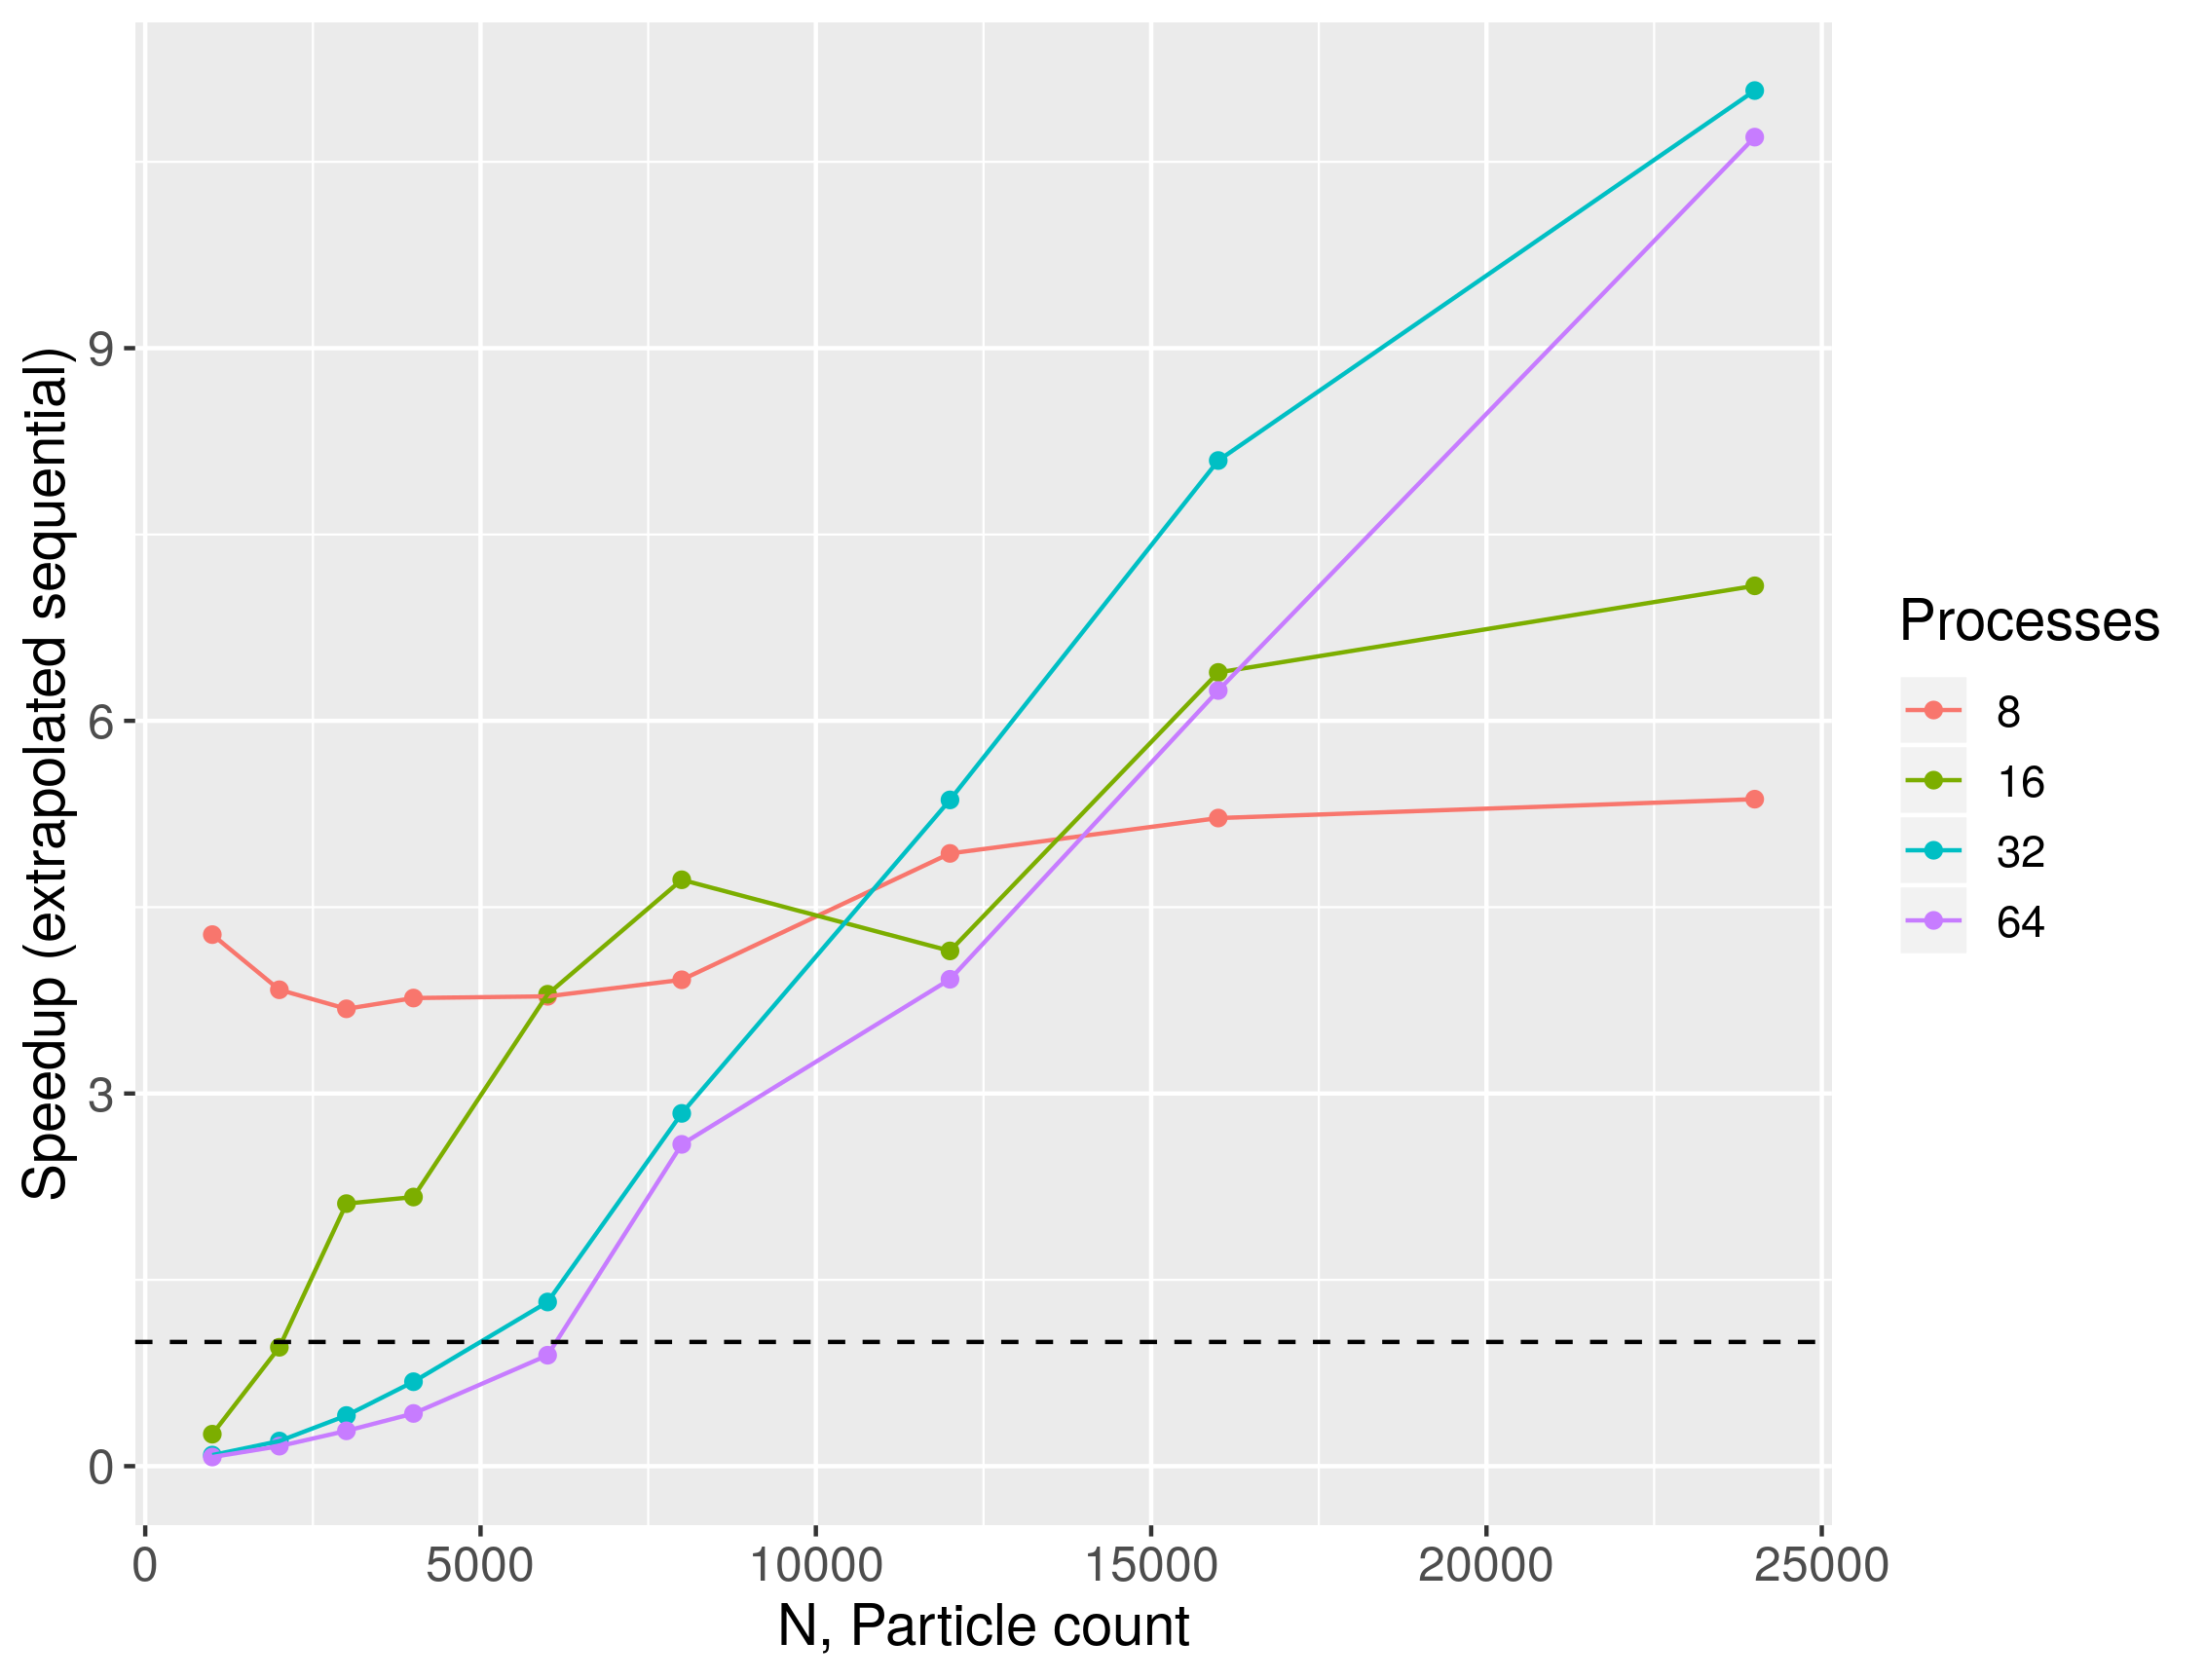
\includegraphics[width=0.74\textwidth]{processedCpuResults/PureI7-seqSpeedup.png}
    \caption{Plot of speedup against $N$ for varying processes (i7-7700K configuration)}
    \label{fig:PureI7-seqSpeedup}
\end{figure}

\pagebreak

\section{Discussion: MPI Implementation}
\label{section:mpi-discussion}

\subsection{Expectations}
Akin to the OpenMP implementation, we expect our MPI implementation for a given number of processes $P$ to exhibit an increasing speedup with increasing $N$ up to some peak value, demonstrating the benefits of parallelisation.\\

However, communication between MPI processes and coordination between the master and slaves will introduce significant overhead that is quantifiable in the overall execution time. Therefore, we additionally expect:
\begin{enumerate}[label=(\arabic*)]
\item The peak speedup for the MPI implementation with $P$ processes to be lower than the equivalent OpenMP implementation with $P$ threads, and 
\item The curve of speedup against $N$ to grow significantly slower towards the peak speedup, as the ratio of computation to communication increases with $N$
\end{enumerate}

Furthermore, when the number of processes $P$ is large and the problem size $N$ is small, we expect the communication overhead to dominate computation time, resulting in potentially worse performance than the sequential implementation.

\subsection{Conclusions}
\label{subsection:mpi-conclusions}

Figures \ref{fig:PureXeS-varyNandProcesses} and \ref{fig:PureI7-varyNandProcesses} demonstrate an interesting mix of behaviour with different regimes for different number of nodes $M$ and problem size $N$.\\

When the number of nodes $M$ is small ($M \leq 2$), we observe that the execution time grows approximately quadratically with the number of particles $N$, for both node configurations. This agrees with our expectations of the execution time being dominated by the computation required for particle-particle collision checks.\\

The peak speedup for small $M$ achieved by both configurations approached the number of processes $P$. This indicates that for our task and data decomposition pattern, the optimal problem size $N$ that balanced computation time and communication overhead was within our range of testcases.\\

\pagebreak

However, the behaviour of the curve of speedup against $N$ differs significantly between $M = 1$ and $M = 2$, for both configurations. When $M = 1$, the speedup begins close to the peak value at $N = 1000$ and plateaus quickly as $N$ increases, remaining close to the peak speedup throughout. In contrast, for $M = 2$, the speedup begins close to $1$ (dotted horizontal line), and then rapidly increases up to $N = 8000$, after which it levels out and approaches the peak speedup asymptotically.\\

This behaviour demonstrates that the cost of communicating across multiple nodes is significant, even for two nodes. When $M = 1$, all processes are confined to the same node and message-passing does not involve the network, leading to relatively little overhead. As a result, the curve of speedup resembles that of the equivalent OpenMP implementation. However, when $M = 2$, the network is now involved in communication operations between processes on different nodes, introducing additional overhead from packet routing and network congestion. Therefore, the curve of speedup begins close to 1 and rapidly increases with $N$, as the ratio of computation to communication changes as more work is assigned to each slave with larger $N$. Notably, there was a small performance regression (speedup $< 1$) for small $N$ on the Intel i7-7700K configuration with $M = 2$.\\

The same trends are not observed with $M \geq 4$ nodes. For small $N$, we observed a huge performance regression (speedup $\ll 1$) relative to the sequential results, with the execution time up to $N = 6k$ being orders-of-magnitude worse than the equivalent execution time with fewer nodes.\\

We attribute this observation to the combination of a small problem size $N$ with a large number of processes $P$. Under such conditions, the tasks assigned to each slave was too granular and required little work, skewing the ratio of execution time heavily towards communication operations instead of computation. This introduced a large amount of network contention from the many slaves attempting to communicate, resulting in much greater overhead. The performance was also further worsened by bottlenecking from the master process, which performs a fair amount of computation alongside its coordination role. This demonstrates the need to carefully select the data distribution and the number of processes $P$ to fit a given problem size $N$.

\pagebreak

Interestingly, this performance regression resolves itself dramatically moving from $N = 6k$ to $N = 8k$, with a marked reduction in execution time observed across both configurations for $N \geq 4$. The execution time continues to increase with greater $N$, but not in a predictable manner, since the curve begins to exhibit signs of plateauing around $N = 16k$. This crossover point at $N = 6k$ between the two regimes also marks the beginning whereby a speedup over the sequential result was observed with the MPI implementation. However, whilst the curve of speedup beyond $N = 6k$ showed a general increasing trend with $N$, it was also similarly unpredictable and exhibited localised deviations.\\

For the Xeon 4114 configuration, we suspect the large communication overhead from the many processes on many distinct nodes ($M \geq 4$) will prevent the peak speedup from approaching the 33x peak speedup observed for two nodes, even in the limit of large $N$.\\

Implementing the particle simulation with MPI boasts a clear advantage over the alternatives. Whilst the OpenMP and CUDA implementations are constrained by the available system and GPU memory respectively, the MPI implementation allows the computation to be scaled transparently across a variable number of computing nodes, allowing the simulation to be run for a much greater number of particles $N$ in a respectable time.\\

However, we opine that this is not the key strength of the message-passing programming model, since the performance of a master-slave pattern will be heavily constrained by the network bandwidth. Instead, we believe that message-passing is best suited for problems with some element of spatial structure with no clear master-slave relationship. This allows efficient mapping of spatial elements in the problem to the underlying topology of the network, ensuring related elements are on nodes in close physical proximity, which will both minimise the latency of message-passing and the bandwidth utilisation from communication operations.

\pagebreak

\section{Discussion: Comparison with OpenMP and CUDA}

\subsection{Remarks on Previous Implementations}
The extrapolated execution times for the sequential implementation in Figure \ref{fig:seqExtrapolate} more clearly showcase the difference in single-core performance between the Xeon Silver 4114 and the Intel i7-7700K. Due to its higher clock frequency, each core of the i7-7700K has a computational throughput about $28\%$ greater than each core of the Xeon Silver 4114.\\

Figures \ref{fig:gpu-speedupI7} and \ref{fig:gpu-speedupXeS} plot the speedup of the CUDA implementation relative to the extrapolated sequential times for varying $N$. Both the Titan RTX and Tesla T4 only possess 2 FP64 units per streaming multiprocessor (SM) \cite{turingarchi}, for a total of 144 and 80 FP64 units respectively.\\

Despite each CUDA core being simpler and less powerful than a single CPU core, we observed a peak speedup (relative to the i7-7700K) of 210 and 130 respectively on the two GPUs, greater than the number of FP64 units. We opine this demonstrates the high \textbf{latency-hiding} capability of GPUs, which are able to exploit their large register file on each SM to switch between occupant threads at a very low cost to minimise stalling.

\subsection{Comparison with OpenMP}
\label{subsection:omp-vs-mpi}

For a fair comparison between OpenMP and MPI, we compare the speedup for the same number of OpenMP threads and MPI processes with varying $N$. The results for both parallel programming models are plotted together in Figures \ref{fig:PureI7-seqSpeedupWithOpenMP} (Intel i7-7700K) and \ref{fig:PureXeS-seqSpeedupWithOpenMP} (Xeon Silver 4114).\\

\pagebreak

\begin{figure}[H]
    \centering
    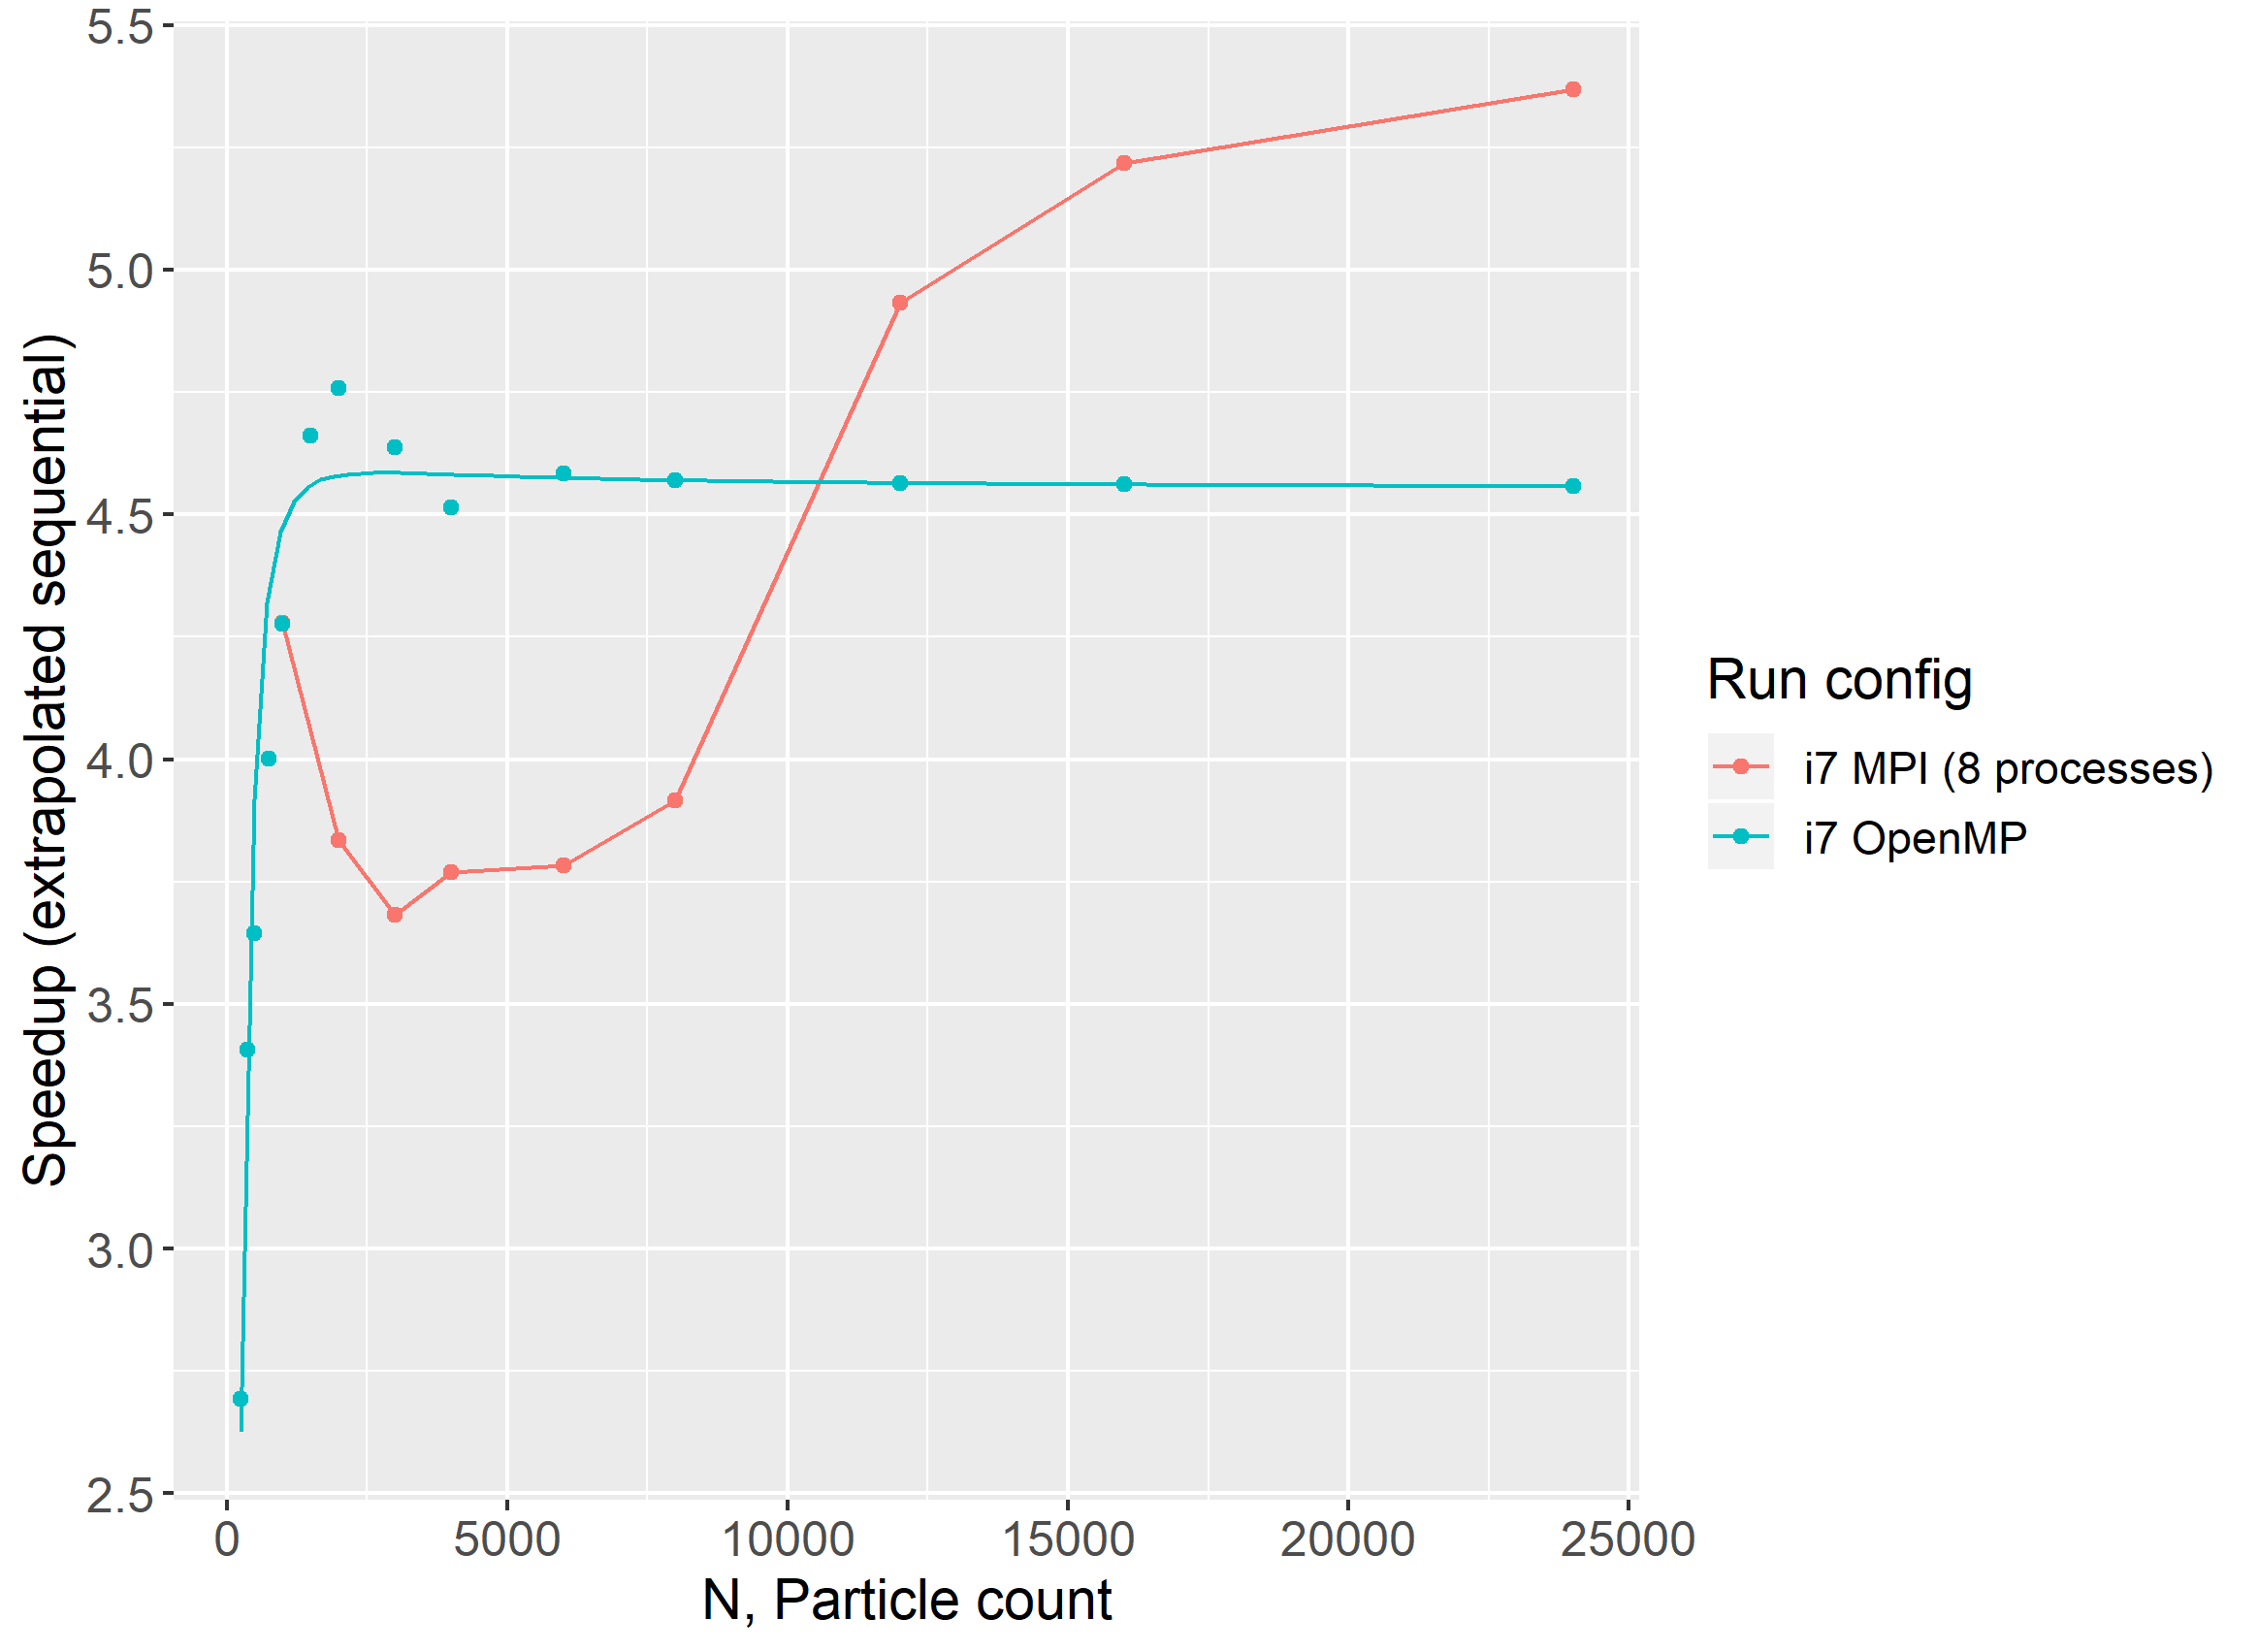
\includegraphics[width=0.8\textwidth]{processedCpuResults/PureI7-seqSpeedupWithOpenMP.png}
    \caption{Plot of speedup against $N$ for 8 OpenMP threads/MPI processes (Intel i7-7700K)}
    \label{fig:PureI7-seqSpeedupWithOpenMP}
\end{figure}

\begin{figure}[H]
    \centering
    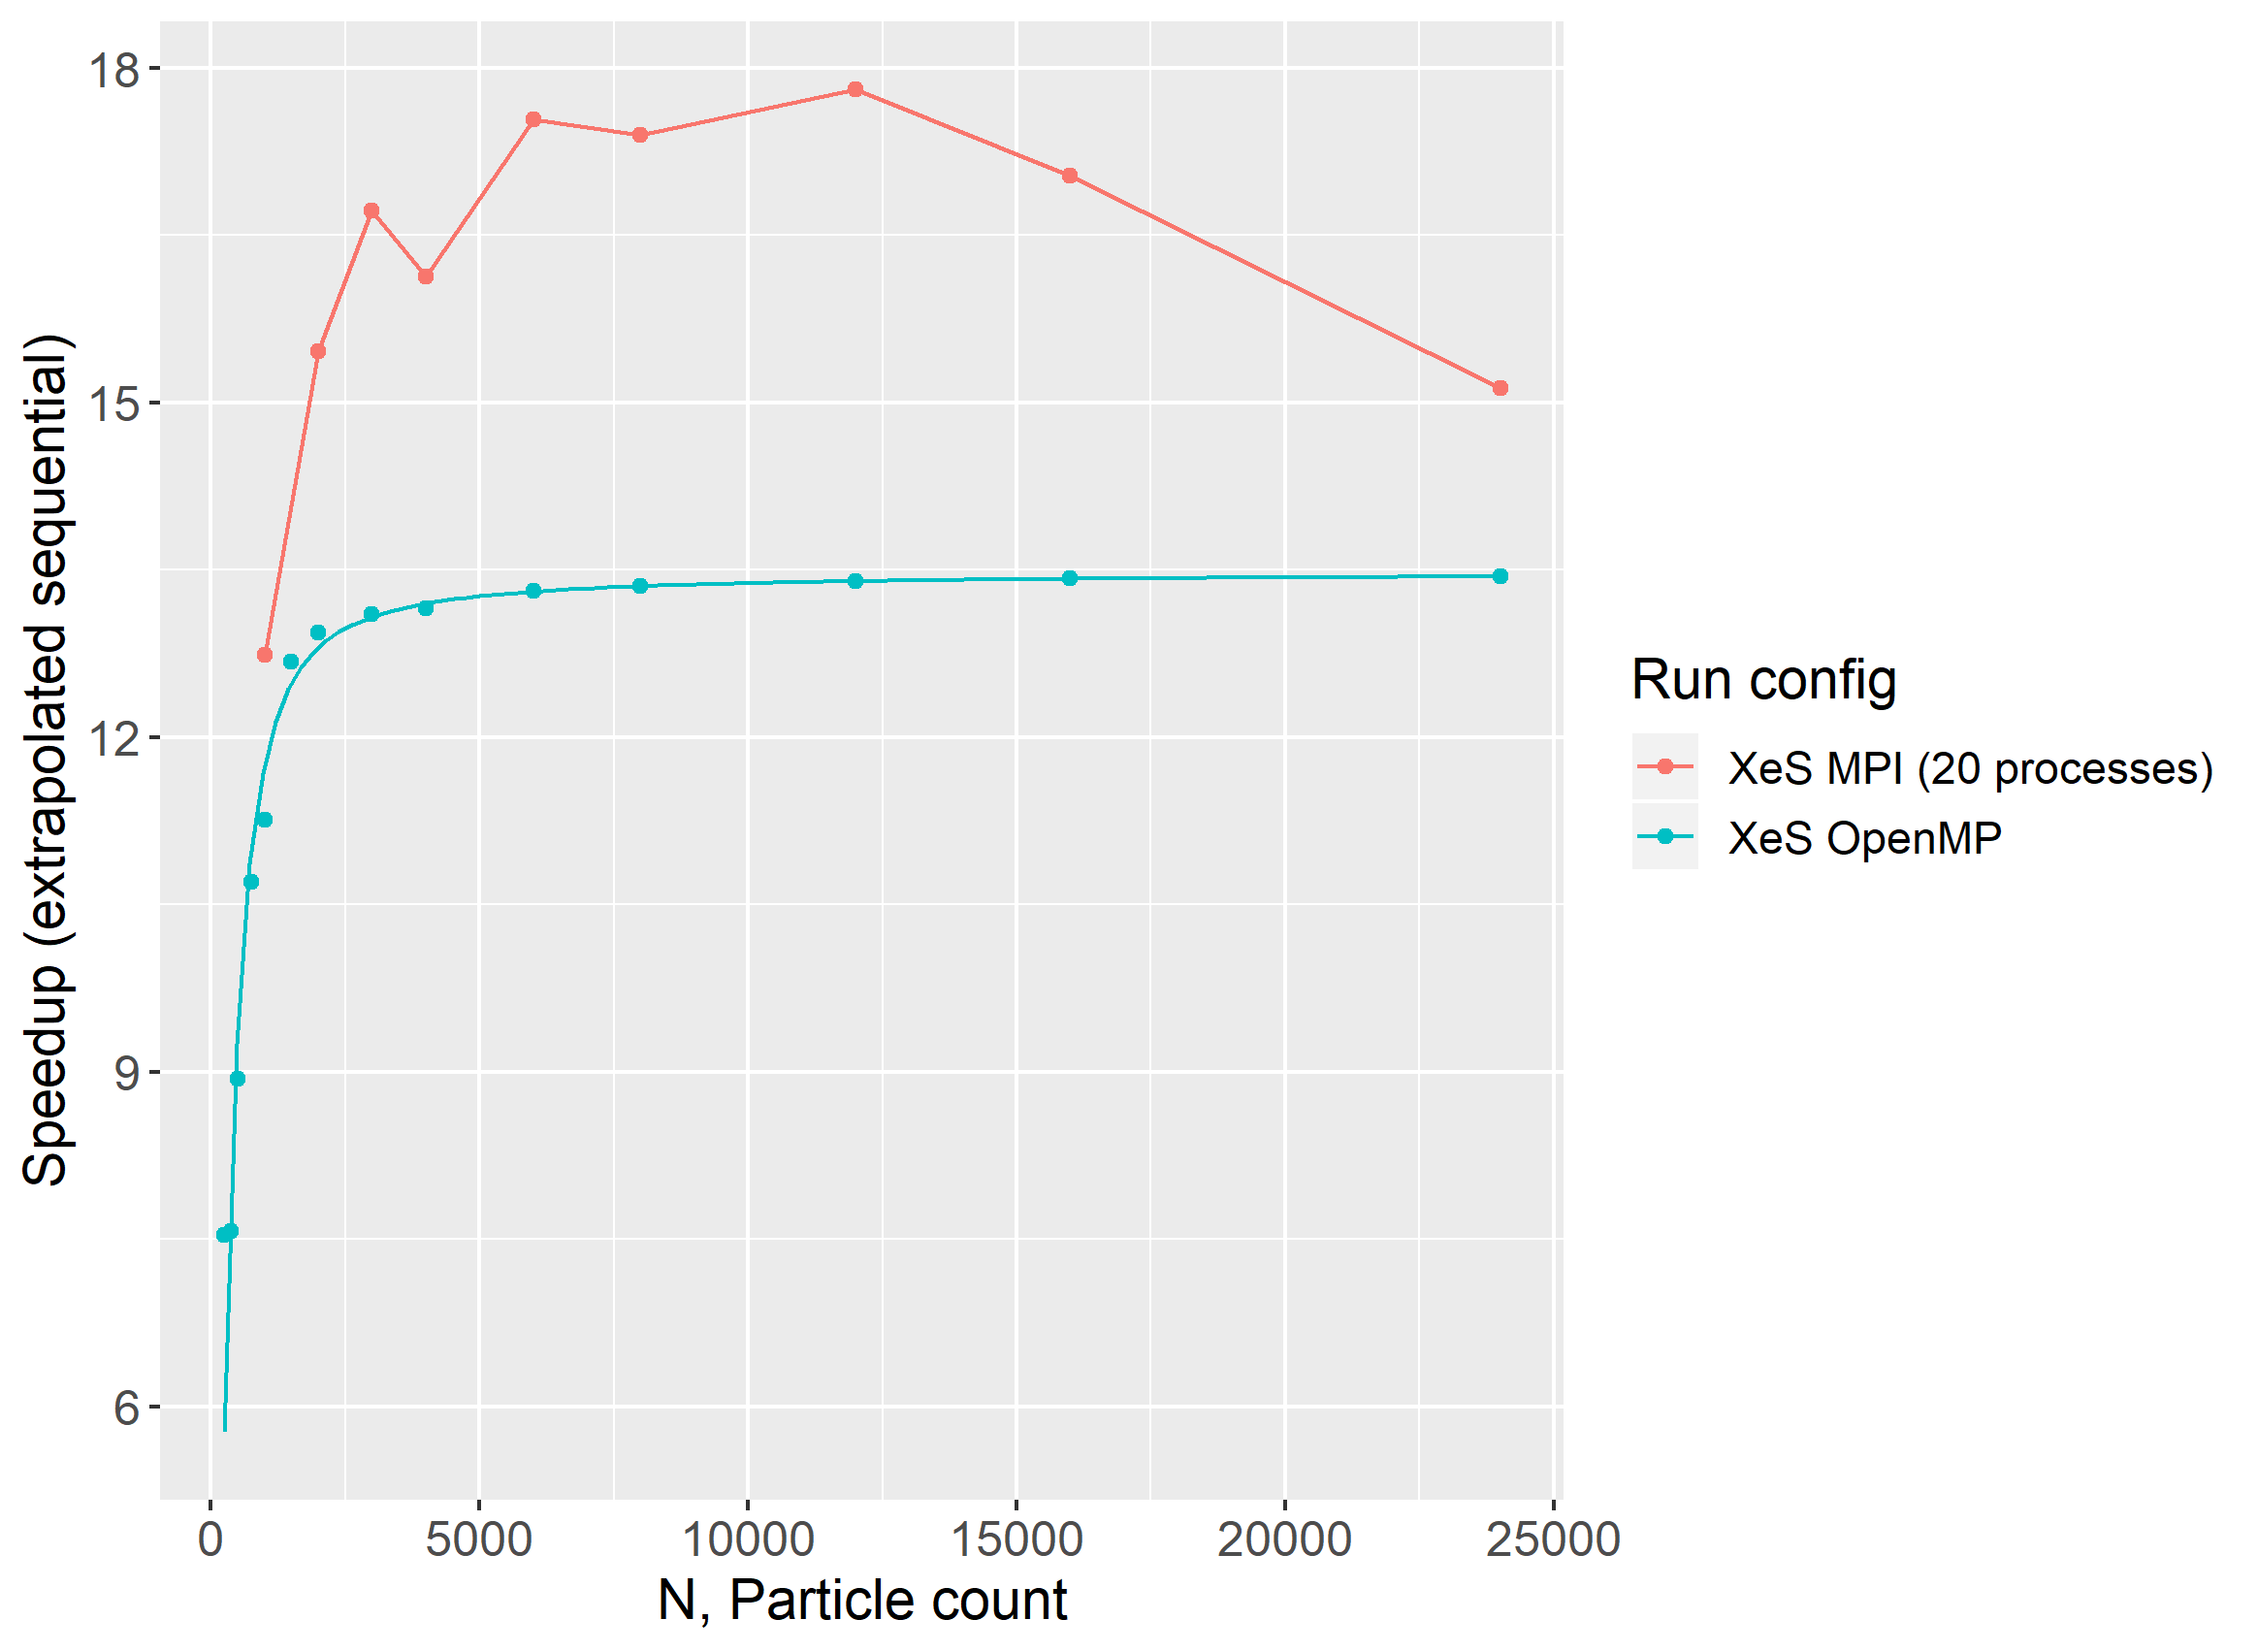
\includegraphics[width=0.8\textwidth]{processedCpuResults/PureXeS-seqSpeedupWithOpenMP.png}
    \caption{Plot of speedup against $N$ for 20 OpenMP threads/MPI processes (Xeon Silver 4114)}
    \label{fig:PureXeS-seqSpeedupWithOpenMP}
\end{figure}

Several observations can be drawn from these two graphs. For the same number of threads/processes, the peak speedup achieved by MPI exceeds that of OpenMP for both machines. However, the speedup for MPI only approaches this maximum value at moderately large problem sizes $N$, in contrast to OpenMP where the speedup attains this peak value early and remains remains close thereafter.\\

We attribute these observations to the differing nature of the programming models:
\begin{enumerate}[label=(\arabic*)]
\item Initial gradient of speedup curve
\begin{itemize}
    \item For OpenMP, the speedup rises quickly towards the peak value at small $N$ due to the benefits of parallelisation
    \item For MPI, the small problem size $N$ leads to tasks that are too finely divided, resulting in the communication overhead dominating the computation time, leading to the curve of speedup growing more slowly towards the peak value
\end{itemize}
\item Peak speedup attainable
\begin{itemize}
    \item For OpenMP, the peak speedup attained is lower due to contention between multiple OpenMP threads for the single critical section to add a collision candidate
    \item For MPI, there are no shared resources between MPI processes except for the network; however, since all MPI processes are confined to the same node, communication operations do not incur additional overhead from the network and hence the peak speedup achieved is greater
\end{itemize}
\item Sensitivity of speedup to problem size $N$
\begin{itemize}
    \item For OpenMP, we see the speedup generally remains close to the peak value after attaining it, since the density of particle-particle collisions dominates with large $N$
    \item For MPI, we see the speedup varies noticeably with problem size $N$, demonstrating the sensitivity of the execution time to the task and data distribution pattern
\end{itemize}
\end{enumerate}

Furthermore, we observe that the speedup of the MPI implementation exhibited a trough between $N = 1k$ to $N = 8k$ - we suspect this occurred due to the greater single-core performance of the i7-7700K processor, which skews the ratio of computation to communication more heavily towards the latter.

\subsection{Comparison with CUDA}

Since CPU and GPU computing are wholly different computing platforms, it is difficult to draw a fair comparison between the CUDA and MPI implementations.\\

However, the empirical benchmarks demonstrate that the highly parallel nature of GPUs provide the CUDA implementation a significant advantage in performance, due to the GPU's high latency-hiding capability. Furthermore, GPUs are able to exploit the high degree of data parallelism in the simulation (since the same task is repeated on many different pieces of data), allowing it to achieve \textbf{superlinear speedup} despite the heavily divergent nature of the computation.
\pagebreak

\section{Discussion: CUDA FP64 performance on the Titan V}

\subsection{Rationale}
In the previous assignment \cite{assign1bref}, we analysed the performance of our CUDA implementation on two Nvidia GPUs, namely the Tesla T4 and the Titan RTX. In particular, we observed that when the implementation was switched to using lower-precision \texttt{float}s from \texttt{double}s, the performance improvement exhibited did not agree with our expectations from the specifications of the FP32 and FP64 FLOPS performance of the GPUs. Only a modest speedup of $2 - 3$ was observed between the two variants, instead of 32 (the ratio of the FP32 : FP64 throughput). \\

We decided to investigate this further with the Titan V, a datacentre-class GPU that boasts the full 32 hardware FP64 units per SM. This gives the Titan V the maximum available FP64 instruction throughput, at half that of the FP32 throughput. The testcases ran on the Titan V did not change from the previous assignment.

\subsection{Titan V Results}

\begin{figure}[H]
    \centering
    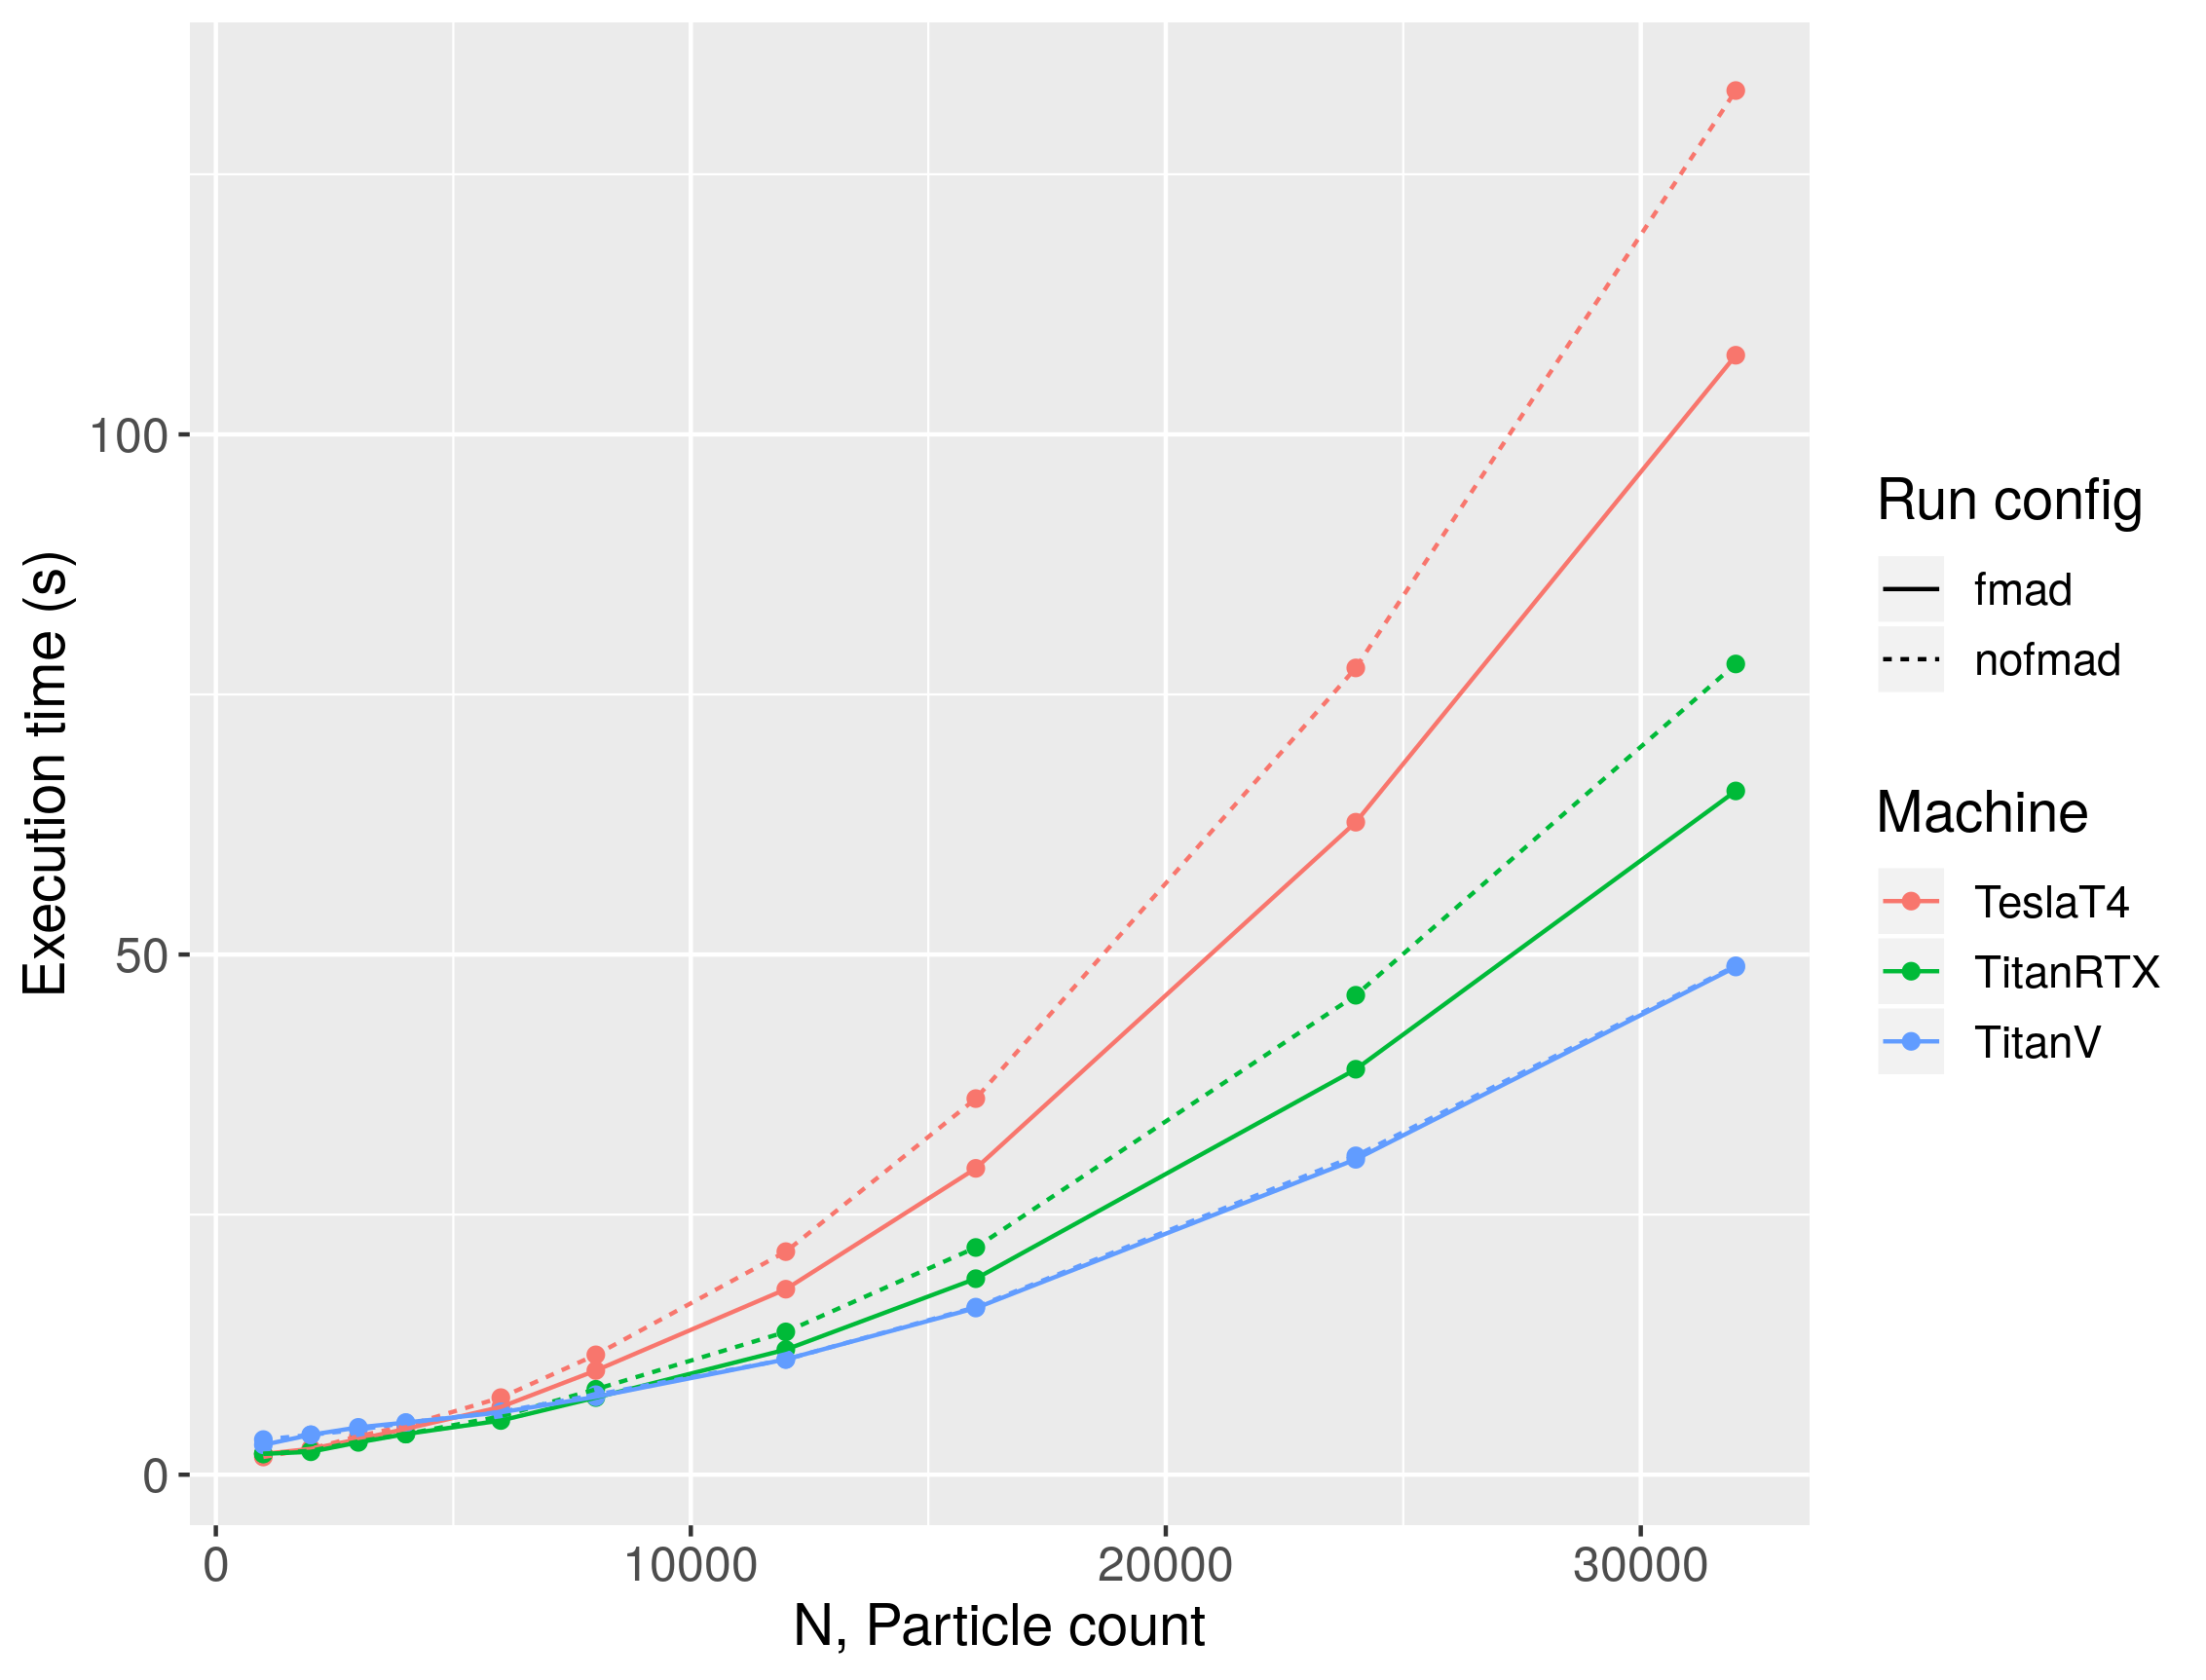
\includegraphics[width=0.75\textwidth]{gpu-varyN}
    \caption{Plot of execution time against particle count, $N$}
    \label{fig:gpu-varyN}
\end{figure}

\begin{figure}[H]
    \centering
    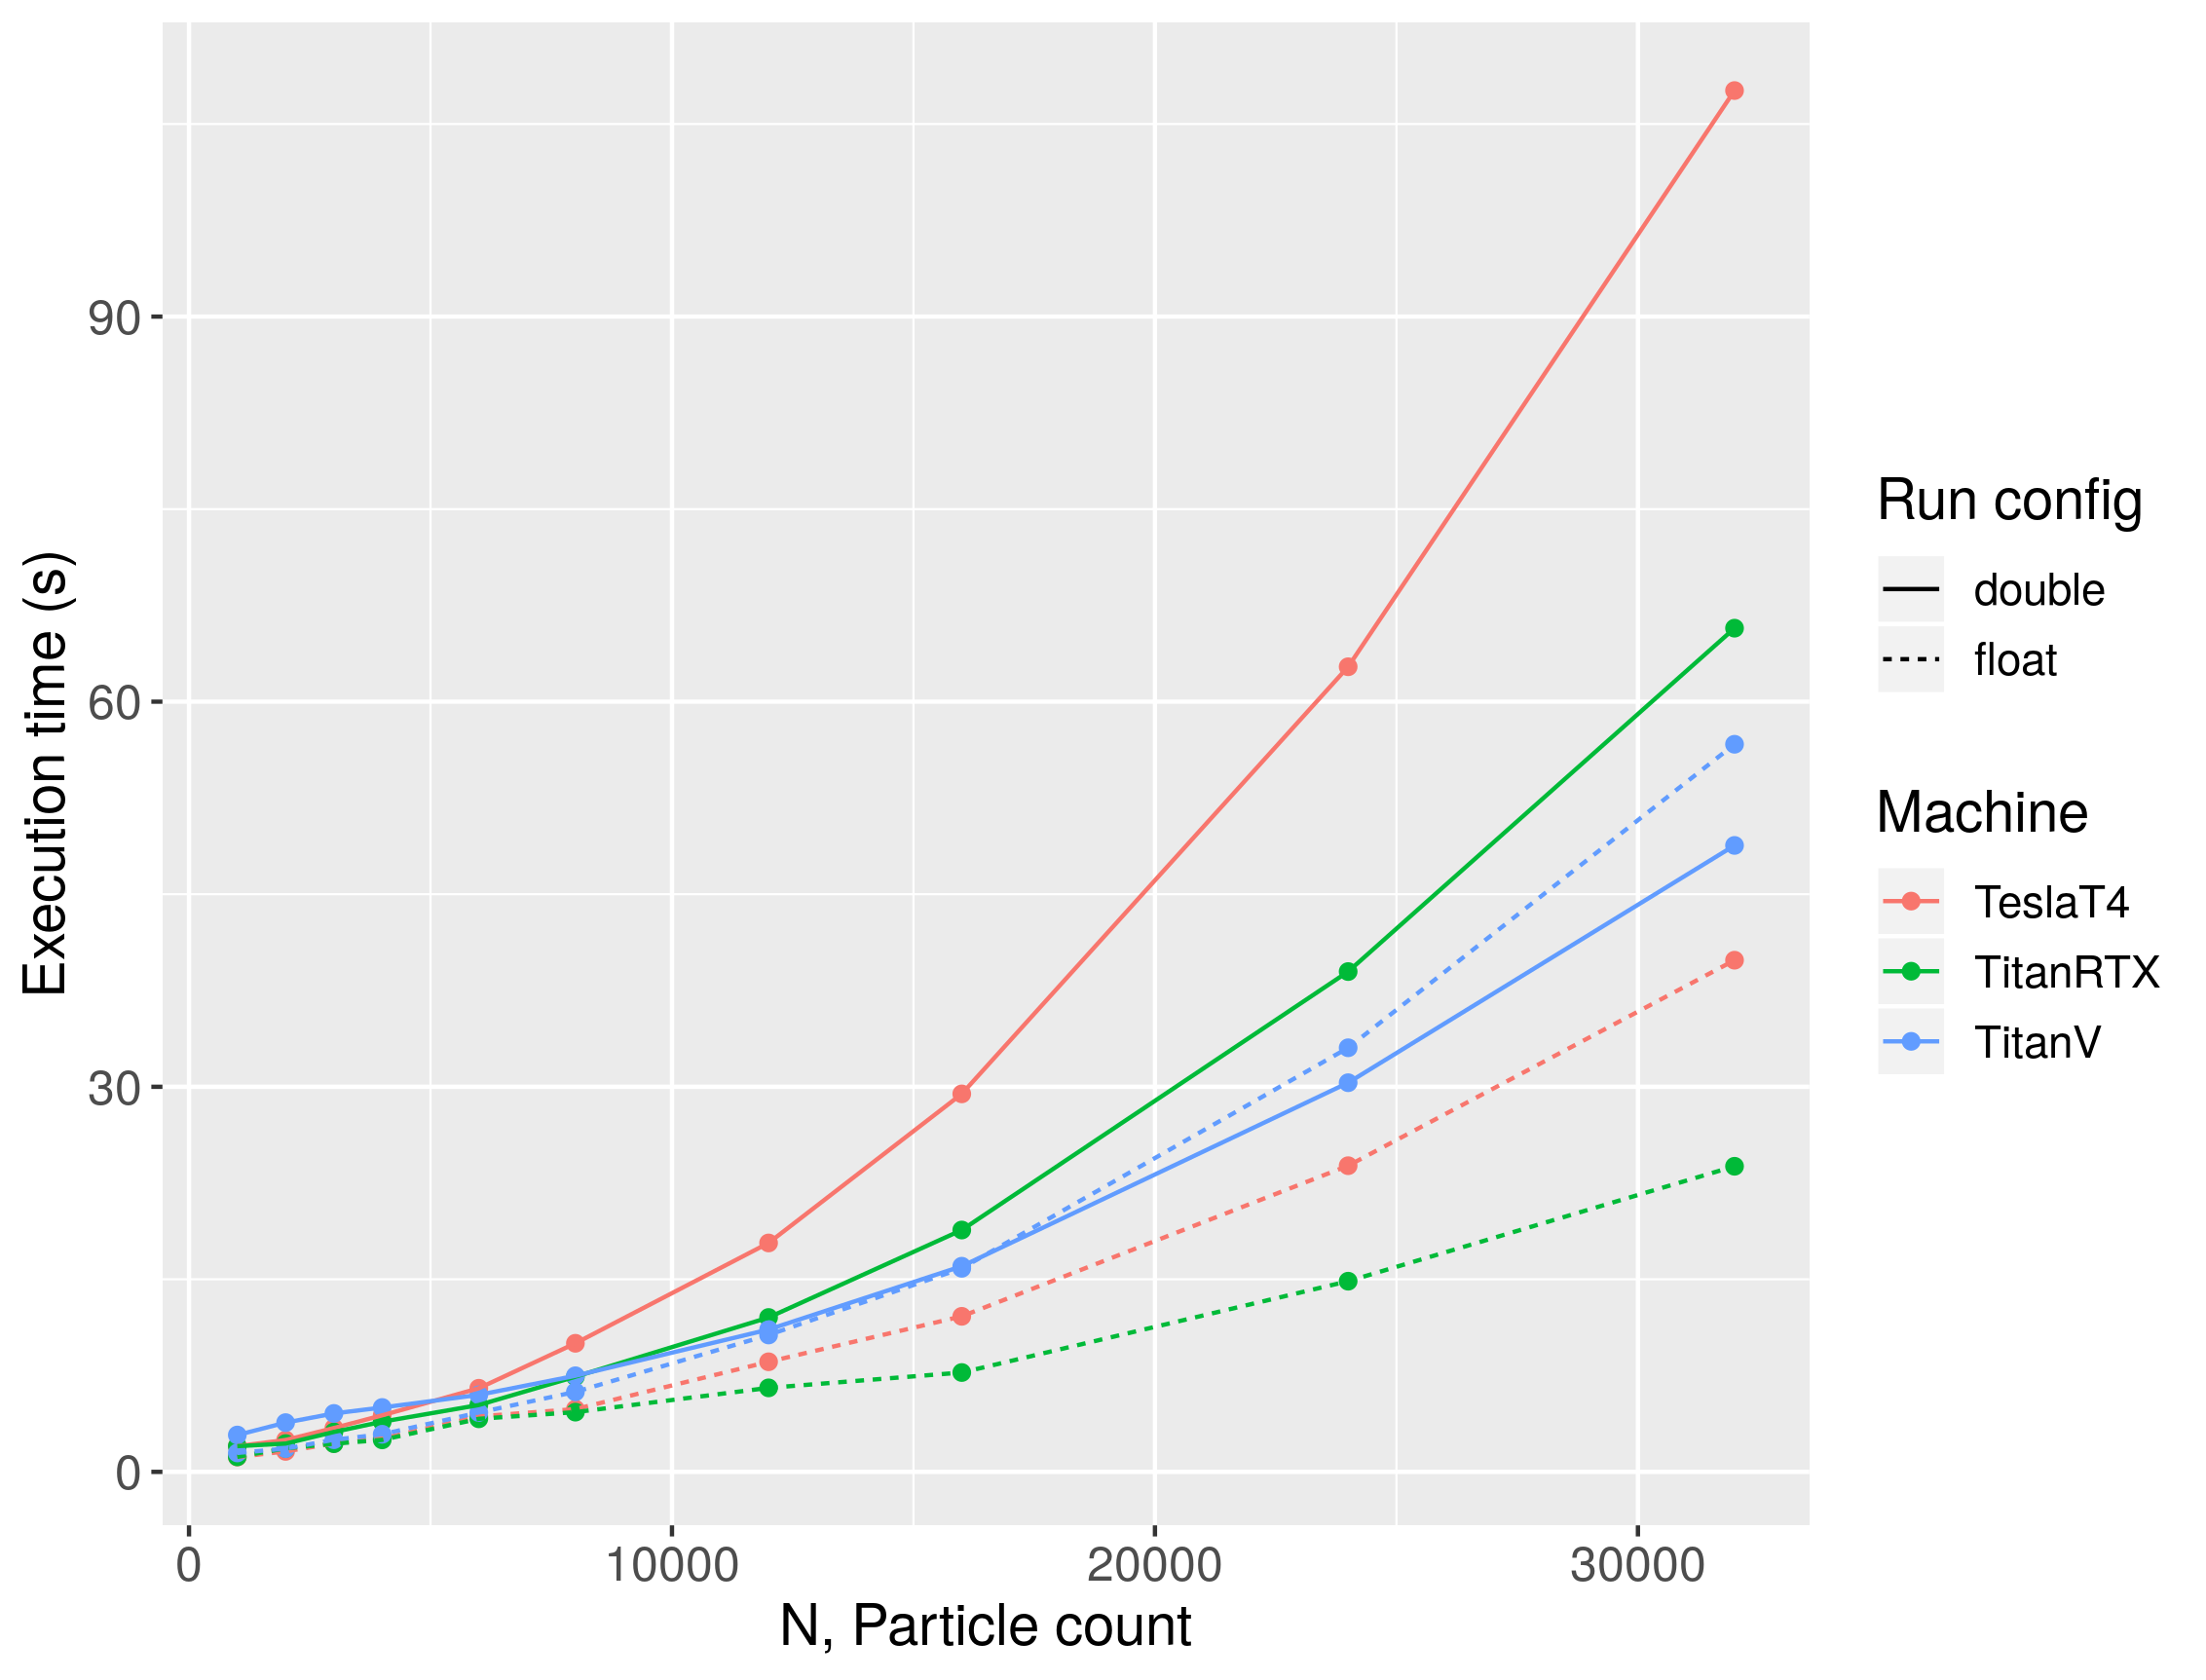
\includegraphics[width=0.75\textwidth]{double-float-comparison-fmad}
    \caption{Plot of execution time (s) against $N$ for \texttt{float} and \texttt{double} programs (\texttt{--fmad=true})}
    \label{fig:double-float-comparison-fmad}
\end{figure}

\begin{figure}[H]
    \centering
    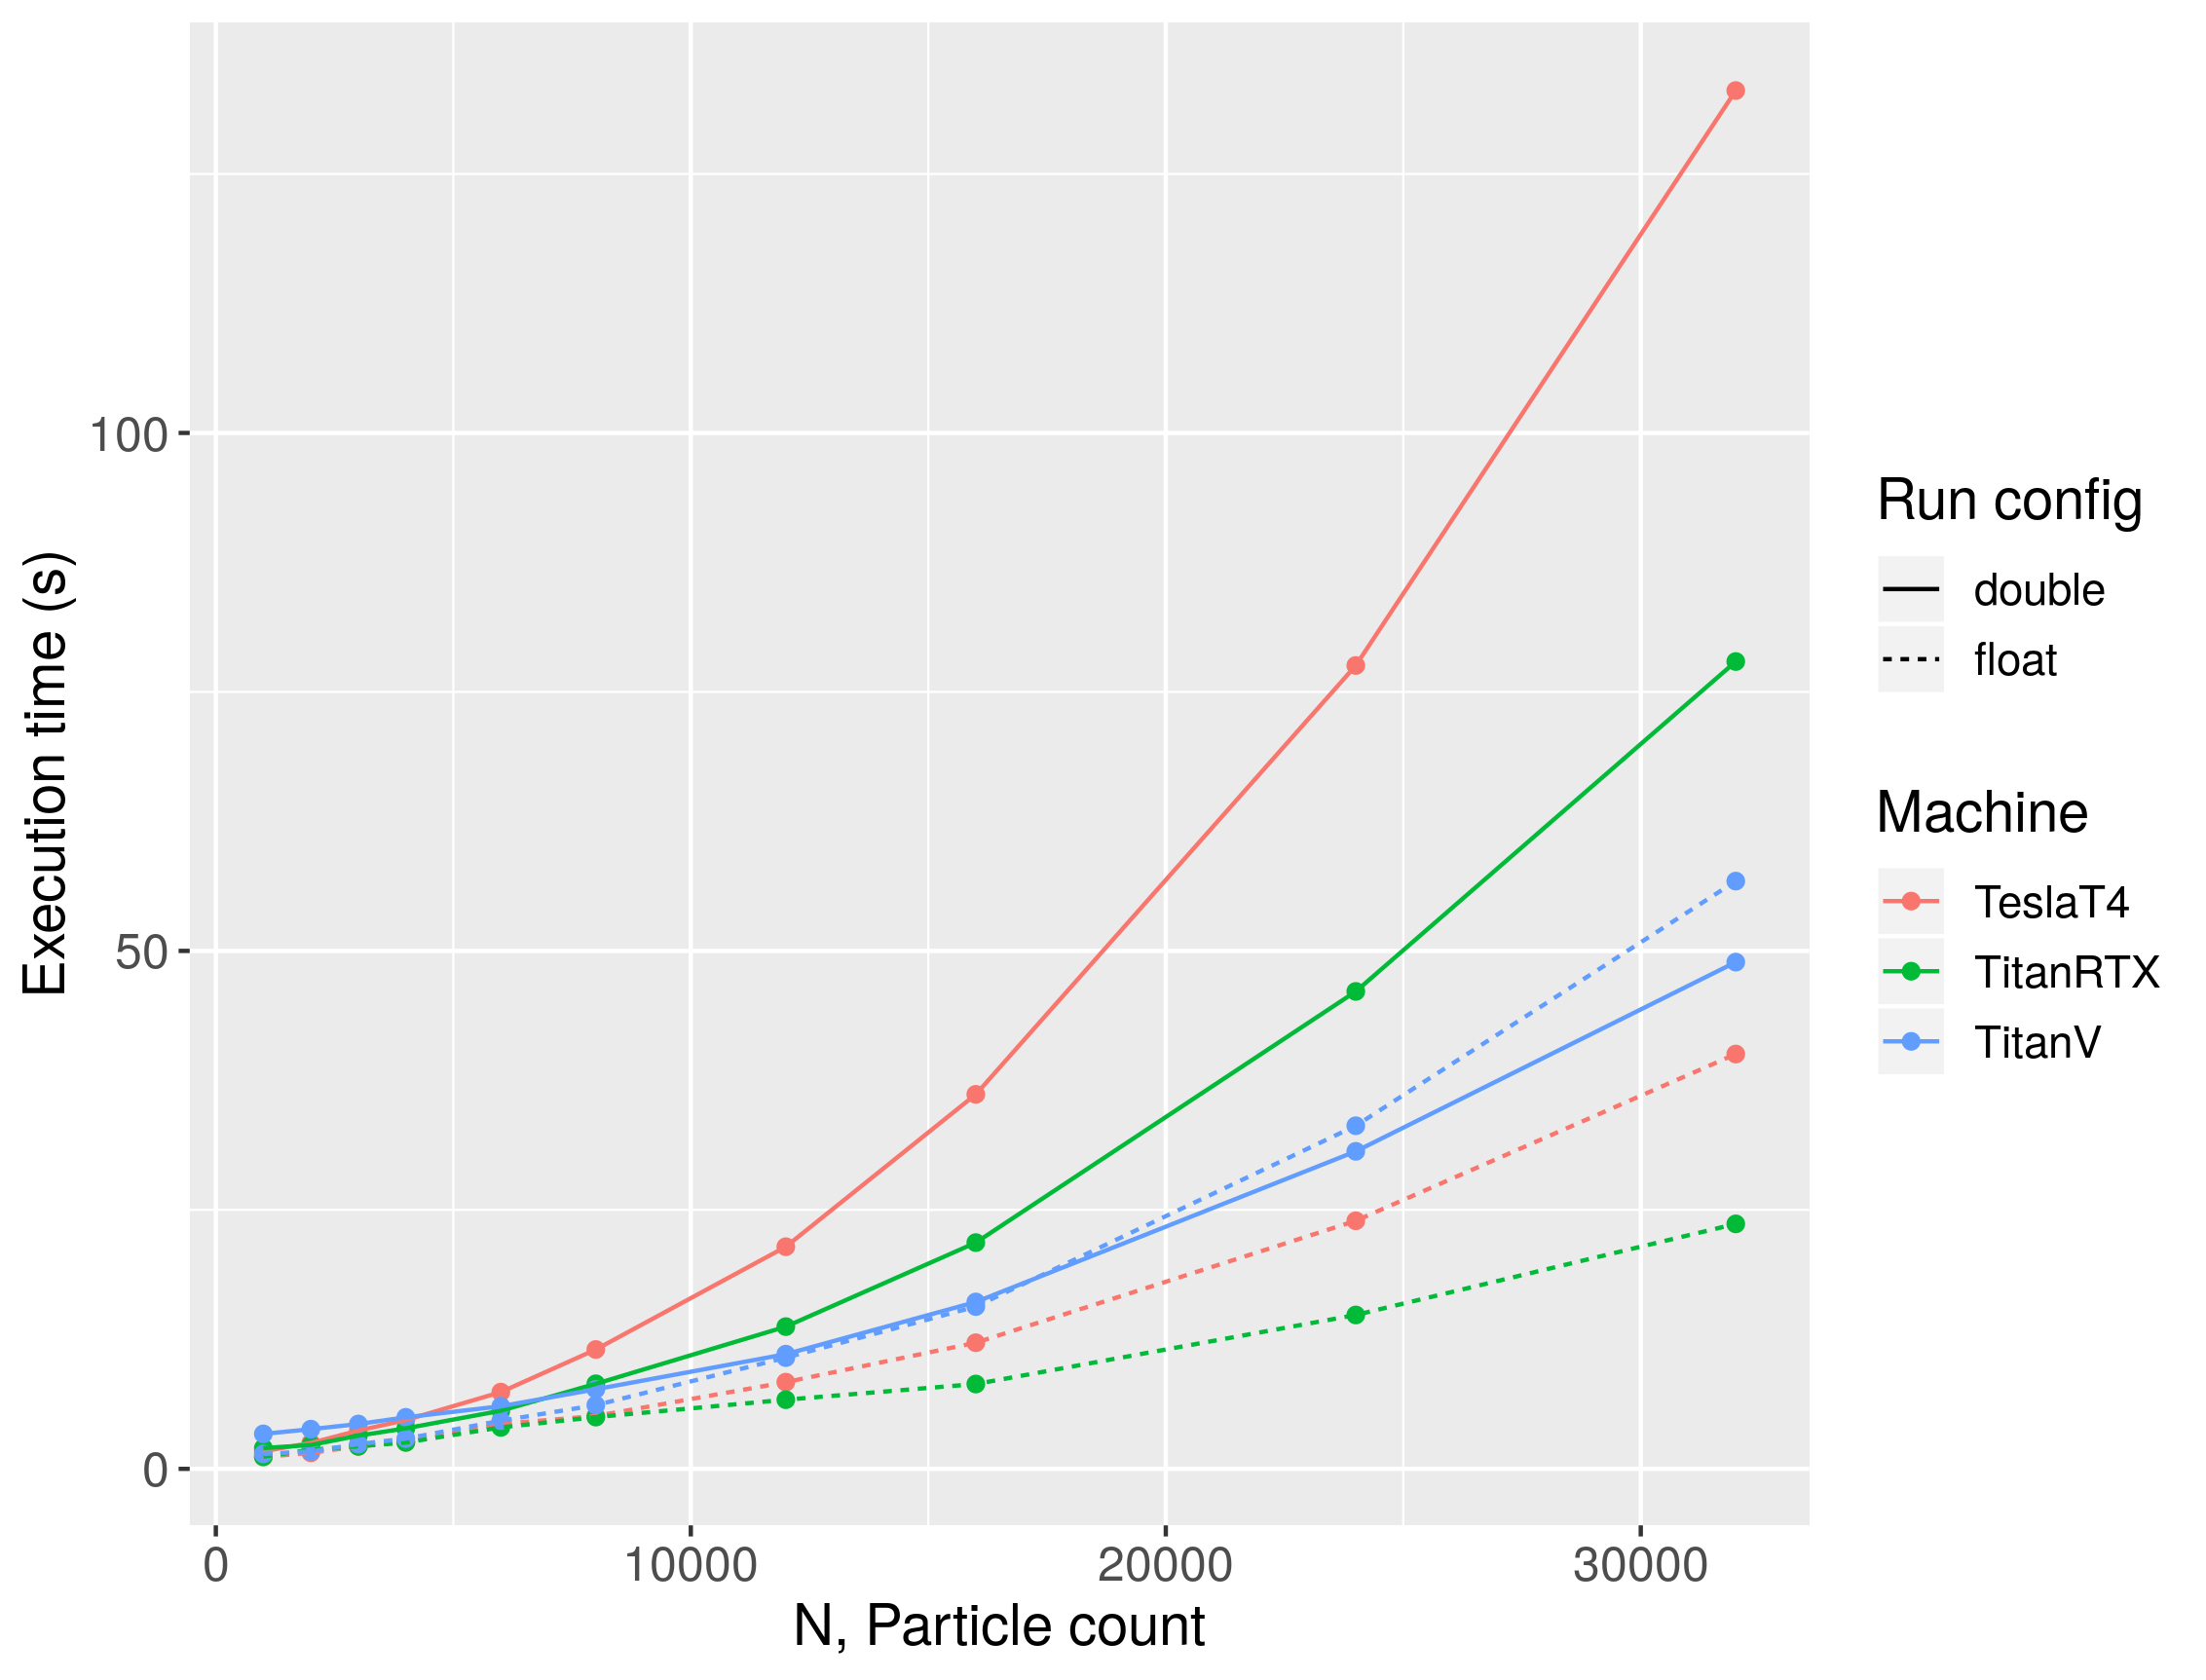
\includegraphics[width=0.75\textwidth]{double-float-comparison-nofmad}
    \caption{Plot of execution time (s) against $N$ for \texttt{float} and \texttt{double} programs (\texttt{--fmad=false})}
    \label{fig:double-float-comparison-nofmad}
\end{figure}

Figure \ref{fig:gpu-varyN} shows that the the presence or absence of the FMA optimisation had little to no effect on the execution time of our CUDA implementation on the Titan V, in contrast to the other two GPUs. We suspect that this occurs due to more severe bottlenecking from the Titan V's memory subsystem, due to its slightly lower memory bandwidth (651.3 GB/s vs. 672.0 GB/s for the Titan RTX) making it more difficult to feed the much larger number of FP64 units with data. As a result, both variants run with a similar execution time, and the effect of the FMA optimisation becomes indiscernible.\\

In contrast, on the other two consumer-grade GPUs, the small number of FP64 units meant that the effect of the FMA optimisation became significantly more pronounced. Since the FMA optimisation reduces the average number of floating-point instructions required for computation, this increases the rate the FP64 units are fed with data, resulting in a small but significant speedup over the non-FMA variant.\\

Figures \ref{fig:double-float-comparison-fmad} and \ref{fig:double-float-comparison-nofmad} shows two interesting observations. First, the performance of the \texttt{float} variant scaled worse on the Titan V with increasing $N$, relative to the other two GPUs. Second, we see that when $N \geq 24k$, the \texttt{double} variant began to perform better than the lower-precision \texttt{float} variant on the Titan V, in deviation to the trend exhibited by the other two GPUs.\\

We attribute both of these observations to a different set of hardware and firmware optimisations on the Titan V GPU, which should favour double-precision FP64 computation over single-precision FP32 computation.\\ 

The Titan RTX and Titan V have a similar number of SMs, at 72 and 80 respectively, but the Titan V has the full number of hardware FP64 units. Between the two, we thus expect the execution time of the \texttt{double} variant to be significantly faster due to the greater number of hardware resources. However, comparing the execution time directly shows that the Titan V only exhibited a modest (relative) speedup of 1.55, failing to reach the factor of 32 that we had expected. We treat this as clear evidence of limitations imposed by the bandwidth of the memory subsystem and the highly divergent nature of discrete particle simulation.

\pagebreak

\section{Potential Optimisations}

\subsection{Hybrid OpenMP-MPI approach}

Our conclusions in section \ref{subsection:mpi-conclusions} suggest that the MPI implementation will likely scale very poorly to a large number of MPI processes on physically distinct nodes, due to limitations of the network bandwidth. This is particularly important since such particle simulations are common in scientific research and are typically run for an extremely large number of particles ($N \gtrapprox 1M$) on a large cluster of computing nodes ($M \gtrapprox 1000)$, such as those of a supercomputer.\\

Since the message-passing model does not possess any problem-specific advantages for discrete particle simulation, we opine that the computation on a node need not be carried out across separate MPI processes.\\

Instead, we propose that a hybrid implementation combining both OpenMP and MPI is best suited for this problem, as it allows us to take advantage of the strengths of both programming models. The modifications required for this are:
\begin{itemize}
    \item Our program will now only create 1 MPI process for each node, for a total of $P$ processes across $P$ nodes; one of these nodes will be designated the master
    \item The master node distributes work between itself and the $P - 1$ slaves; each process then parallelises the computation of its tasks with OpenMP
    \item OpenMP directives are used to (1) perform parallel execution by creating a team of threads of size equal to the number of logical cores on that node, and (2) to enforce synchronisation between OpenMP threads\\
\end{itemize}

The benefits of such a hybrid approach are:
\begin{itemize}
    \item Retaining MPI's ability to scale the computation across multiple physical computing nodes
    \item Reducing overall communication overhead, since a smaller number of MPI processes result in fewer communication operations required and thus less network contention
    \item Retaining the memory footprint advantage from OpenMP, as the use of shared memory avoids the need to replicate portions of the simulation state across many independent MPI processes
\end{itemize}

\subsection{Optimising Communication Operations}
Figure \ref{fig:PureXeS-varyNandProcesses} demonstrates how network contention from many MPI processes participating in collective communication operations may lead to significant performance regression. To address this, we propose that reworking the message-passing between the master and slaves may improve the performance by reducing the strain on the network in transmitting data.\\

The changes would include:
\begin{enumerate}[label=(\arabic*)]
\item The master only transmitting the section of the particle array required by each slave for checking particle-particle collisions, instead of broadcasting the entire array of $N$ particles
\item The master transmitting only the additional particles required by each slave for collision resolution
\item Replacing the collective communication operations with their non-blocking variants where safe, allowing processes to perform computation to hide the latency of message-passing
\end{enumerate}

\subsection{Optimising Collision-sorting}
Presently, the master process is responsible for sorting all the gathered collision candidates in its own \texttt{cs} array, which we have shown in our previous report \cite{assign1bref} to have complexity of $O(N^2\:lg\,N)$ with quicksort, where $N$ is the number of particles.\\

Therefore, it is possible to reduce the execution time by optimising this sorting of collisions. A parallel sorting algorithm (e.g. parallel mergesort) could be employed with all $P$ processes to distribute the task of sorting amongst the slaves, reducing the time required for the sorting to be completed by the master process.
\pagebreak

\bibliography{references}
\bibliographystyle{abbrv}

\end{document}
